%%%%%%%%%%%%%%%%%%%%%%%%%%%%%%%%%%%%%%%%%%%%%%%%%%%%%%%%%%%%%%%%%%%%%%%%%%%%%%%%%
% Template: Article
%
% Por: Abrantes Araújo Silva Filho
%      abrantesasf@gmail.com
%
% Citação: Se você gostou deste template, por favor ajude a divulgá-lo mantendo
%          o link para meu repositório GitHub em:
%          https://github.com/abrantesasf/LaTeX
%%%%%%%%%%%%%%%%%%%%%%%%%%%%%%%%%%%%%%%%%%%%%%%%%%%%%%%%%%%%%%%%%%%%%%%%%%%%%%%%%




%%%%%%%%%%%%%%%%%%%%%%%%%%%%%%%%%%%%%%%%%%%%%%%%%%%%%%%%%%%%%%%%%%%%%%%%%%%%%%%%%
%%% Configura o tipo de documento, papel, tamanho da fonte e informações básicas
%%% para as proriedades do PDF/DVIPS e outras propriedades do documento
\RequirePackage{ifpdf}
\ifpdf
  % Classe, língua e tamanho da fonte padrão. Outras opções a considerar:
  %   draft
  %   onecolumn (padrão) ou twocolumn (OU usar o package multicol)
  %   fleqn com ou sem leqno (alinhamento à esquerda das fórmulas e dos números)
  %   oneside (padrão para article ou report) ou twoside (padrão para book)
  \documentclass[pdftex, brazil, 12pt, twoside]{article}
\else
  % Classe, língua e tamanho da fonte padrão. Outras opções a considerar:
  %   draft
  %   onecolumn (padrão) ou twocolumn (OU usar o package multicol)
  %   fleqn com ou sem leqno (alinhamento à esquerda das fórmulas e dos números)
  %   oneside (padrão para article ou report) ou twoside (padrão para book)
  \documentclass[brazil, 12pt]{article}
\fi


%%%%%%%%%%%%%%%%%%%%%%%%%%%%%%%%%%%%%%%%%%%%%%%%%%%%%%%%%%%%%%%%%%%%%%%%%%%%%%%%%
%%% Carrega pacotes iniciais necessários para estrutura de controle e para a
%%% criação e o parse de novos comandos
\usepackage{ifthen}
\usepackage{xparse}


%%%%%%%%%%%%%%%%%%%%%%%%%%%%%%%%%%%%%%%%%%%%%%%%%%%%%%%%%%%%%%%%%%%%%%%%%%%%%%%%%
%%% Configuração do tamanho da página, margens, espaçamento entrelinhas e, se
%%% necessário, ativa a indentação dos primeiros parágrafos.
\ifpdf
  \usepackage[pdftex]{geometry}
\else
  \usepackage[dvips]{geometry}
\fi
\geometry{a4paper, left=2.6cm, right=4.0cm, top=3.0cm, bottom=3.4cm}

\usepackage{setspace}
  \singlespacing
  %\onehalfspacing
  %\doublespacing


%%%%%%%%%%%%%%%%%%%%%%%%%%%%%%%%%%%%%%%%%%%%%%%%%%%%%%%%%%%%%%%%%%%%%%%%%%%%%%%%%
%%% Configurações de cabeçalho e rodapé:
\usepackage{fancyhdr}
\setlength{\headheight}{1cm}
\setlength{\footskip}{1.5cm}
\renewcommand{\headrulewidth}{0.3pt}
\renewcommand{\footrulewidth}{0.0pt}
\pagestyle{fancy}
\renewcommand{\sectionmark}[1]{%
  \markboth{\uppercase{#1}}{}}
\renewcommand{\subsectionmark}[1]{%
  \markright{\uppercase{\thesubsection \hspace{0.1cm} #1}}{}}
\fancyhead{}
\fancyfoot{}
\newcommand{\diminuifonte}{%
    \fontsize{9pt}{9}\selectfont
}
\newcommand{\aumentafonte}{%
    \fontsize{12}{12}\selectfont
}
% Configura cabeçalho e rodapé para documentos TWOSIDE
\fancyhead[EL]{\textbf{\thepage}}
\fancyhead[EC]{}
\fancyhead[ER]{\diminuifonte \textbf{\leftmark}}
\fancyhead[OR]{\textbf{\thepage}}
\fancyhead[OC]{}
\fancyhead[OL]{\diminuifonte \textbf{\rightmark}}
\fancyfoot[EL,EC,ER,OR,OC,OL]{}
% Configura cabeçalho e rodapé para documentos ONESIDE
%\lhead{ \fancyplain{}{sup esquerdo} }
%\chead{ \fancyplain{}{sup centro} }
%\rhead{ \fancyplain{}{\thesection} }
%\lfoot{ \fancyplain{}{inf esquerdo} }
%\cfoot{ \fancyplain{}{inf centro} }
%\rfoot{ \fancyplain{}{\thepage} }




%%%%%%%%%%%%%%%%%%%%%%%%%%%%%%%%%%%%%%%%%%%%%%%%%%%%%%%%%%%%%%%%%%%%%%%%%%%%%%%%%
%%% Configurações de encoding, lingua e fontes:
\usepackage[T1]{fontenc}
\usepackage[utf8]{inputenc}
\usepackage{babel}

% Altera a fonte padrão do documento (nem todas funcionam em modo math):
%   phv = Helvetica
%   ptm = Times
%   ppl = Palatino
%   pbk = bookman
%   pag = AdobeAvantGarde
%   pnc = Adobe NewCenturySchoolBook
\renewcommand{\familydefault}{ppl}


%%%%%%%%%%%%%%%%%%%%%%%%%%%%%%%%%%%%%%%%%%%%%%%%%%%%%%%%%%%%%%%%%%%%%%%%%%%%%%%%%
%%% Carrega pacotes para referências cruzadas, citações dentro do documento,
%%% links para internet e outros.Configura algumas opções.
%%% Não altere a ordem de carregamento dos packages.
\usepackage{varioref}
\ifpdf
  \usepackage[pdftex]{hyperref}
    \hypersetup{
      % Informações variáveis em cada documento (MUDE AQUI!):
      pdftitle={Calculus 1A: Differentiation},
      pdfauthor={MITx on EdX},
      pdfsubject={MITx 18.01.1x on EdX --- Calculus 1A: Differentiation},
      pdfkeywords={calculus, derivative},
      pdfinfo={
        CreationDate={}, % Ex.: D:AAAAMMDDHH24MISS
        ModDate={}       % Ex.: D:AAAAMMDDHH24MISS
      },
      % Coisas que você não deve alterar se não souber o que está fazendo:
      unicode=true,
      pdflang={pt-BR},
      bookmarksopen=true,
      bookmarksnumbered=true,
      bookmarksopenlevel=5,
      pdfdisplaydoctitle=true,
      pdfpagemode=UseOutlines,
      pdfstartview=FitH,
      pdfcreator={LaTeX with hyperref package},
      pdfproducer={pdfTeX},
      pdfnewwindow=true,
      colorlinks=true,
      citecolor=green,
      linkcolor=red,
      filecolor=cyan,
      urlcolor=blue
    }
\else
  \usepackage{hyperref}
\fi
\usepackage{cleveref}
\usepackage{url}


%%%%%%%%%%%%%%%%%%%%%%%%%%%%%%%%%%%%%%%%%%%%%%%%%%%%%%%%%%%%%%%%%%%%%%%%%%%%%%%%%
%%% Carrega bibliotecas de símbolos (matemáticos, físicos, etc.), fontes
%%% adicionais, e configura algumas opções
\usepackage{amsmath}
\usepackage{amssymb}
\usepackage{amsfonts}
\usepackage{siunitx}
  \sisetup{group-separator = {.}}
  \sisetup{group-digits = {false}}
  \sisetup{output-decimal-marker = {,}}
\usepackage{bm}
\usepackage{cancel}
% Altera separador decimal via comando, se necessário (prefira o siunitx):
%\mathchardef\period=\mathcode`.
%\DeclareMathSymbol{.}{\mathord}{letters}{"3B}
  

%%%%%%%%%%%%%%%%%%%%%%%%%%%%%%%%%%%%%%%%%%%%%%%%%%%%%%%%%%%%%%%%%%%%%%%%%%%%%%%%%
%%% Carrega packages relacionados à computação
\usepackage{algorithm2e}
\usepackage{algorithmicx}
\usepackage{algpseudocode}
\usepackage{listings}
  \lstset{literate=
    {á}{{\'a}}1 {é}{{\'e}}1 {í}{{\'i}}1 {ó}{{\'o}}1 {ú}{{\'u}}1
    {Á}{{\'A}}1 {É}{{\'E}}1 {Í}{{\'I}}1 {Ó}{{\'O}}1 {Ú}{{\'U}}1
    {à}{{\`a}}1 {è}{{\`e}}1 {ì}{{\`i}}1 {ò}{{\`o}}1 {ù}{{\`u}}1
    {À}{{\`A}}1 {È}{{\'E}}1 {Ì}{{\`I}}1 {Ò}{{\`O}}1 {Ù}{{\`U}}1
    {ä}{{\"a}}1 {ë}{{\"e}}1 {ï}{{\"i}}1 {ö}{{\"o}}1 {ü}{{\"u}}1
    {Ä}{{\"A}}1 {Ë}{{\"E}}1 {Ï}{{\"I}}1 {Ö}{{\"O}}1 {Ü}{{\"U}}1
    {â}{{\^a}}1 {ê}{{\^e}}1 {î}{{\^i}}1 {ô}{{\^o}}1 {û}{{\^u}}1
    {Â}{{\^A}}1 {Ê}{{\^E}}1 {Î}{{\^I}}1 {Ô}{{\^O}}1 {Û}{{\^U}}1
    {œ}{{\oe}}1 {Œ}{{\OE}}1 {æ}{{\ae}}1 {Æ}{{\AE}}1 {ß}{{\ss}}1
    {ű}{{\H{u}}}1 {Ű}{{\H{U}}}1 {ő}{{\H{o}}}1 {Ő}{{\H{O}}}1
    {ç}{{\c c}}1 {Ç}{{\c C}}1 {ø}{{\o}}1 {å}{{\r a}}1 {Å}{{\r A}}1
    {€}{{\euro}}1 {£}{{\pounds}}1 {«}{{\guillemotleft}}1
    {»}{{\guillemotright}}1 {ñ}{{\~n}}1 {Ñ}{{\~N}}1 {¿}{{?`}}1
  }
  

%%%%%%%%%%%%%%%%%%%%%%%%%%%%%%%%%%%%%%%%%%%%%%%%%%%%%%%%%%%%%%%%%%%%%%%%%%%%%%%%%
%%% Ativa suporte extendido a cores
\usepackage[svgnames]{xcolor} % Opções de cores: usenames (16), dvipsnames (64),
                              % svgnames (150) e x11names (300).


%%%%%%%%%%%%%%%%%%%%%%%%%%%%%%%%%%%%%%%%%%%%%%%%%%%%%%%%%%%%%%%%%%%%%%%%%%%%%%%%%
%%% Suporte à importação de gráficos externos
\ifpdf
  \usepackage[pdftex]{graphicx}
\else
  \usepackage[dvips]{graphicx}
\fi


%%%%%%%%%%%%%%%%%%%%%%%%%%%%%%%%%%%%%%%%%%%%%%%%%%%%%%%%%%%%%%%%%%%%%%%%%%%%%%%%%
%%% Suporte à criação de gráficos proceduralmente na LaTeX:
\usepackage{tikz}
  \usetikzlibrary{arrows,automata,backgrounds,matrix,patterns,positioning,shapes,shadows}


%%%%%%%%%%%%%%%%%%%%%%%%%%%%%%%%%%%%%%%%%%%%%%%%%%%%%%%%%%%%%%%%%%%%%%%%%%%%%%%%%
%%% Packages para tabelas
\usepackage{array}
\usepackage{longtable}
\usepackage{tabularx}
\usepackage{tabu}
\usepackage{lscape}
\usepackage{colortbl}  
\usepackage{booktabs}


%%%%%%%%%%%%%%%%%%%%%%%%%%%%%%%%%%%%%%%%%%%%%%%%%%%%%%%%%%%%%%%%%%%%%%%%%%%%%%%%%
%%% Packages ambientes de listas
\usepackage{enumitem}
\usepackage[ampersand]{easylist}


%%%%%%%%%%%%%%%%%%%%%%%%%%%%%%%%%%%%%%%%%%%%%%%%%%%%%%%%%%%%%%%%%%%%%%%%%%%%%%%%%
%%% Packages para suporte a ambientes floats, captions, etc.:
\usepackage{float}
\usepackage{wrapfig}
\usepackage{placeins}
\usepackage{caption}
\usepackage{sidecap}
\usepackage{subcaption}


%%%%%%%%%%%%%%%%%%%%%%%%%%%%%%%%%%%%%%%%%%%%%%%%%%%%%%%%%%%%%%%%%%%%%%%%%%%%%%%%%
%%% Meus comandos específicos:
% Commando para ``italizar´´ palavras em inglês (e outras línguas!):
\newcommand{\ingles}[1]{\textit{#1}}

% Commando para colocar o espaço correto entre um número e sua unidade:
\newcommand{\unidade}[2]{\ensuremath{#1\,\mathrm{#2}}}
\newcommand{\unidado}[2]{{#1}\,{#2}}

% Produz ordinal masculino ou feminino dependendo do segundo argumento:
\newcommand{\ordinal}[2]{%
#1%
\ifthenelse{\equal{a}{#2}}%
{\textordfeminine}%
{\textordmasculine}}


%%%%%%%%%%%%%%%%%%%%%%%%%%%%%%%%%%%%%%%%%%%%%%%%%%%%%%%%%%%%%%%%%%%%%%%%%%%%%%%%%
%%% Hifenização específica quando o LaTeX/Babel não conseguirem hifenizar:
\babelhyphenation{Git-Hub}
\usepackage{exsol}



%%%%%%%%%%%%%%%%%%%%%%%%%%%%%%%%%%%%%%%%%%%%%%%%%%%%%%%%%%%%%%%%%%%%%%%%%%%%%%%%%
%%%%%%%%%%%%%%%%%%%%%%%%%%%%%%%%%%%%%%%%%%%%%%%%%%%%%%%%%%%%%%%%%%%%%%%%%%%%%%%%%
%%%%%%%%%%%%%%%%%%%%%%%%%%%%%%%%%%%%%%%%%%%%%%%%%%%%%%%%%%%%%%%%%%%%%%%%%%%%%%%%%
%%%%%%%%%%%%%%%%%%%%%%%%%%%%%%%%%%%%%%%%%%%%%%%%%%%%%%%%%%%%%%%%%%%%%%%%%%%%%%%%%
%%%%%%%%%%%%%%%%%%%%%%%%%%%%%% COMEÇA O DOCUMENTO %%%%%%%%%%%%%%%%%%%%%%%%%%%%%%%
%%%%%%%%%%%%%%%%%%%%%%%%%%%%%%%%%%%%%%%%%%%%%%%%%%%%%%%%%%%%%%%%%%%%%%%%%%%%%%%%%
%%%%%%%%%%%%%%%%%%%%%%%%%%%%%%%%%%%%%%%%%%%%%%%%%%%%%%%%%%%%%%%%%%%%%%%%%%%%%%%%%
%%%%%%%%%%%%%%%%%%%%%%%%%%%%%%%%%%%%%%%%%%%%%%%%%%%%%%%%%%%%%%%%%%%%%%%%%%%%%%%%%
%%%%%%%%%%%%%%%%%%%%%%%%%%%%%%%%%%%%%%%%%%%%%%%%%%%%%%%%%%%%%%%%%%%%%%%%%%%%%%%%%
\begin{document}
\title{Calculus 1A: Differentiation}
\author{MITx 18.01.1x}
\date{2018/08/17 -- 2018/11/20}
\maketitle
\tableofcontents
\newpage


%%%%%%%%%%%%%%%%%%%%%%%%%%%%%%%%%%%%%%%%%%%%%%%%%%%%%%%%%%%%%%%%%%%%%%%%%%%%%%%%%
%%%%%%%%%%%%%%%%%%%%%%%%%%%%%%%%%%%%%%%%%%%%%%%%%%%%%%%%%%%%%%%%%%%%%%%%%%%%%%%%%
%%%%%%%%%%%%%%%%%%%%%%%%%%%%%%%%%%%%%%%%%%%%%%%%%%%%%%%%%%%%%%%%%%%%%%%%%%%%%%%%%
\section{Getting started (2018/08/17)}
\label{gs}


%%%%%%%%%%%%%%%%%%%%%%%%%%%%%%%%%%%%%%%%%%%%%%%%%%%%%%%%%%%%%%%%%%%%%%%%%%%%%%%%%
%%%%%%%%%%%%%%%%%%%%%%%%%%%%%%%%%%%%%%%%%%%%%%%%%%%%%%%%%%%%%%%%%%%%%%%%%%%%%%%%%
\subsection{Overview and logistics}
\label{gs-ol}

%%%%%%%%%%%%%%%%%%%%%%%%%%%%%%%%%%%%%%%%%%%%%%%%%%%%%%%%%%%%%%%%%%%%%%%%%%%%%%%%%
\subsubsection{Meet the course team}
\label{gs-ol-team}

\paragraph{Professor David Jerison}
David Jerison received his Ph.D.\ from Princeton University in 1980, and joined the mathematics faculty at MIT in 1981. In 1985, he received an A.P.\ Sloan Foundation Fellowship and a Presidential Young Investigator Award. In 1999 he was elected to the American Academy of Arts and Sciences. In 2004, he was selected for a Margaret MacVicar Faculty Fellowship in recognition of his teaching. In 2012, the American Mathematical Society awarded him and his collaborator Jack Lee the Bergman Prize in Complex Analysis.

\begin{figure}[H]
  \begin{center}
    \caption{Professor David Jerison}
    \label{fig:david-jerison}
    \fbox{
\includegraphics[scale=0.7]{imagens/jerison.jpg}}
    %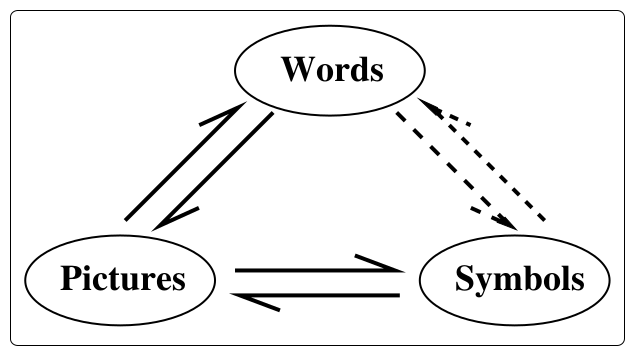
\includegraphics[scale=0.4]{imagens/palavras-imagens-simbolos.png}
    %
    %\footnotesize{Fonte:}
  \end{center}
\end{figure}

Professor Jerison's research focuses on PDEs and Fourier Analysis. He has taught single variable calculus, multivariable calculus, and differential equations at MIT several times each.

\paragraph{Professor Gigliola Staffilan}
Gigliola Staffilani is the Abby Rockefeller Mauzé Professor of Mathematics since 2007. She received her Ph.D.\ from the University of Chicago in 1995. Following faculty appointments at Stanford, Princeton, and Brown, she joined the MIT mathematics faculty in 2002. She received both a teaching award and a research fellowship while at Stanford. She received a Sloan Foundation Fellowship in 2000. In 2014 she was elected to the American Academy of Arts and Sciences.

\begin{figure}[H]
  \begin{center}
    \caption{Professor Gigliola Staffilani}
    \label{fig:gigliola}
    \fbox{
\includegraphics[scale=0.7]{imagens/staffilani.jpg}}
    %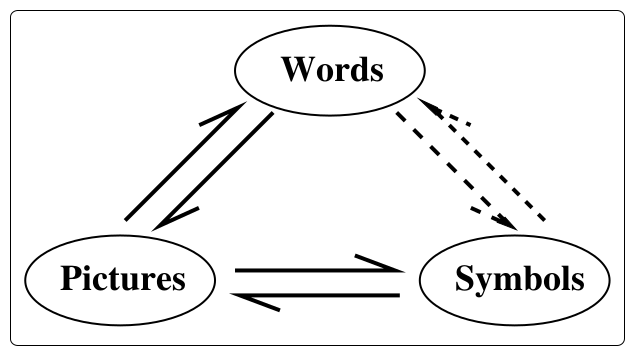
\includegraphics[scale=0.4]{imagens/palavras-imagens-simbolos.png}
    %
    %\footnotesize{Fonte:}
  \end{center}
\end{figure}

Professor Staffilani is an analyst, with a concentration on dispersive nonlinear PDEs. She has taught multivariable calculus several times at MIT, as well as differential equations.

\paragraph{Instructor Jen French}
Jen French is an MITx Digital Learning Scientist in the MIT math department. She earned her Ph.D.\ in mathematics from MIT in 2010, with specialization in Algebraic Topology. After teaching after school math for elementary aged students and working with the Teaching and Learning Lab at MIT developing interdisciplinary curricular videos tying foundational concepts in math and science to engineering design themes, she joined MITx in 2013. She has developed videos, visual interactives, and problems providing immediate feedback using the edX platform residentially in the MIT math department to aid student learning. She has developed the calculus series (3 courses) and differential equations series (5 courses) available here on edX.

\begin{figure}[H]
  \begin{center}
    \caption{Instructor Jen French }
    \label{fig:jen}
    \fbox{
\includegraphics[scale=0.7]{imagens/french.jpg}}
    %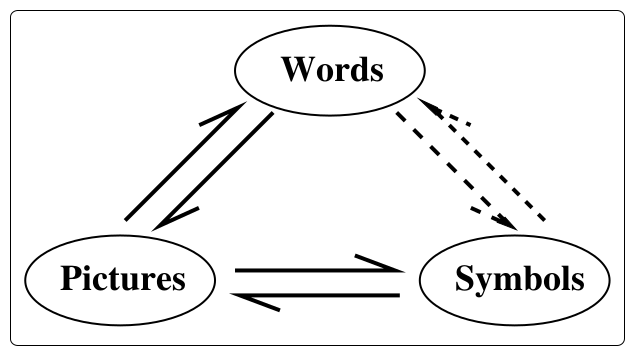
\includegraphics[scale=0.4]{imagens/palavras-imagens-simbolos.png}
    %
    %\footnotesize{Fonte:}
  \end{center}
\end{figure}

\paragraph{Instructor Stephen Wang}
Stephen Wang earned a Ph.D.\ in mathematics from the University of Chicago in 2006, where he specialized in geometry. He has earned teaching awards from both Chicago and Harvard University, and has also been a faculty member at Haverford College and Bucknell University before jumping on board the calculus team at MIT. In fall 2015 he joined the Rice University mathematics faculty.

\begin{figure}[H]
  \begin{center}
    \caption{Instructor Stephen Wang}
    \label{fig:wang}
    \fbox{
\includegraphics[scale=0.7]{imagens/wang.jpg}}
  \end{center}
\end{figure}

\paragraph{Special thanks to \ldots}
Huge thanks to Prof. Arthur Mattuck for starting it all. Big thanks to Timothy Hall for asking David Jerison the question, how do ziplines behave mathematically. We also thank David Custer and Susan Ruff who helped with real life ziplines and shared MIT student experiments on ziplines.

Ed Tech Developers:
\begin{itemize}[noitemsep]
\item J.\ M.\ Claus
\item Brian French
\item Eric Heubel
\item Haynes Miller
\item Martin Segado
\end{itemize}

MIT Undergrads:
\begin{itemize}[noitemsep]
\item Phillip Ai
\item Emanuele Ceccarelli
\item Peter Haine
\item Peter Kleinhenz
\item Mohammed Kane
\end{itemize}

MIT PhD Students:
\begin{itemize}[noitemsep]
\item Tudor Cristea-Platon
\item Kristin Kurianski
\item Lucas Tambasco
\end{itemize}

MITx Video Team:
\begin{itemize}[noitemsep]
\item Brittany Bellamy
\item Chris Boebel
\item Kenny Caudill
\item Tsinu Heramo
\item Jess Kloss
\item Douglass McLean
\item Lana Scott
\item Catilin Stier
\end{itemize}

MITx Support Staff:
\begin{itemize}[noitemsep]
\item Kyle Boots
\item Brad K.\ Goodman
\end{itemize}

\fbox{\begin{minipage}{10cm}This course was funded in part by:\ \\
Class of 1960 Alumni Funds\ \\
2014--2015 Alumni Class Funds Grant\ \\
Wertheimer Fund\end{minipage}}

%%%%%%%%%%%%%%%%%%%%%%%%%%%%%%%%%%%%%%%%%%%%%%%%%%%%%%%%%%%%%%%%%%%%%%%%%%%%%%%%%
\subsubsection{Course description}
\label{gs-ol-description}

Discover the derivative --- what it is, how to compute it, and when to apply it in solving real world problems. Part 1 of 3.

How does the final velocity on a zip line change when the starting point is raised or lowered by a matter of centimeters? What is the accuracy of a GPS position measurement? How fast should an airplane travel to minimize fuel consumption? The answers to all of these questions involve the derivative.

But what is the derivative? You will learn its mathematical notation, physical meaning, geometric interpretation, and be able to move fluently between these representations of the derivative. You will discover how to differentiate any function you can think up, and develop a powerful intuition to be able to sketch the graph of many functions. You will make linear and quadratic approximations of functions to simplify computations and gain intuition for system behavior. You will learn to maximize and minimize functions to optimize properties like cost, efficiency, energy, and power.

This course, in combination with \emph{18.01.2x Calculus 1B: Integration}, covers the AP Calculus AB curriculum.

This course, in combination with \emph{18.01.2x Calculus 1B: Integration} and \emph{18.01.3x Calculus 1C: Coordinate Systems and Infinite Series}, covers the AP Calculus BC curriculum.

If you intend to take an AP exam, we strongly suggest that you familiarize yourself with the AP exam to prepare for it.

%%%%%%%%%%%%%%%%%%%%%%%%%%%%%%%%%%%%%%%%%%%%%%%%%%%%%%%%%%%%%%%%%%%%%%%%%%%%%%%%%
\subsubsection{The making of this course}
\label{gs-ol-making}

This course was created using latex2edX, a free tool developed at MIT for creating content for edX written in \LaTeX. \LaTeX\ is a typesetting language that is fantastic for writing math! Occasionally, the equations you see in the webpage (which are rendered in mathjax) do not load appropriately. Our apologies. The easiest fix is to simply reload the page. Another solution is to change browsers. (Firefox seems to render mathjax less reliably than Chrome or Safari. However, frequent changes to edX will cause disruptions in our content.)

Note edX is not supported on tablet devices. That said, users report that 95\% of the problems can be done on a tablet device, but if weird errors are creeping in (especially with formula input type problems) you may try switching to a laptop or desktop computer.

\begin{figure}[H]
  \begin{center}
    %\caption{}
    \label{fig:latex2edx}
    \fbox{
\includegraphics[scale=0.7]{imagens/latex2edx.png}}
  \end{center}
\end{figure}
 
%%%%%%%%%%%%%%%%%%%%%%%%%%%%%%%%%%%%%%%%%%%%%%%%%%%%%%%%%%%%%%%%%%%%%%%%%%%%%%%%%
\subsubsection{How to succeed}
\label{gs-ol-succeed}

\paragraph{Prerequisites}
This course has a global audience with students from a wide variety of backgrounds. To succeed in this course, you must have a solid foundation in

\begin{enumerate}[noitemsep]
\item Algebra
\item Geometry
\item Trigonometry
\item Exponents
\item Logarithms
\item Limits
\end{enumerate}

We know that many students may not have solid foundation in limits, so we have included an optional Unit 0 that introduces Limits. Understanding limits is essential to understand the first lecture on the definition of the derivative in Unit 1, some Homework problems on Continuity and Differentiability in Unit 1, and the first lecture on Limiting behavior and sketching functions in Unit 4.

Because we know you come from different backgrounds, we want to help you to choose the best path through this content. To aid us in this, please take the ``Choose your calculus adventure'' diagnostics. This will help you to determine if you have the skills to succeed, what skills you may need to review, and which units you may be able to skip!

\paragraph{Reference materials}
The material we provide in the Courseware contains all of the content you need for this course. However, there are many good calculus texts that have a great deal of problems and alternate explanations that may help you. Most widely used calculus texts are adequate.

There is also the free web resource \href{https://www.khanacademy.org/}{Khan Academy}.
Links to other web resources can be found on the Course Info page under the header ``Related Links''. Feel free to share other resources on the course wiki or through the discussion forum.

%%%%%%%%%%%%%%%%%%%%%%%%%%%%%%%%%%%%%%%%%%%%%%%%%%%%%%%%%%%%%%%%%%%%%%%%%%%%%%%%%
\subsubsection{Grading}
\label{gs-ol-grading}

There are 4 categories of graded problems in 18.01.1x: in-lecture Exercises, Part A Homework, Part B Homework, and the Final Exam.

\begin{itemize}
\item \textbf{Exercises:} These are the problems that are interspersed between videos in each lecture. These problems count for 20\% of your grade. These problems will be used to motivate theory, practice a concept you just learned, and review material from previous sequences that we are using. While you are graded on these problems, they are low-stakes: you have multiple attempts, and have the opportunity to look at the answer after you have submitted a correct answer or run out of attempts. This is where you will do the majority of your learning. We encourage you to make mistakes and learn from them!
\item \textbf{Part A Homework:} Each unit has 1 Part A Homework assignment, which gives you an opportunity to practice what you learned. These problems count for 10\% of your total grade. Wait until the end of the unit to attempt these problems. These problems help you identify the concepts that you have forgotten, and aid in long-term retention. These problems are mostly mechanical–asking you to practice methods, and techniques learned in each unit. Each problem typically tests knowledge from only one section in a unit. (We won't necessarily tell you which one though!)
\item \textbf{Part B Homework:} Each unit has 1 Part B Homework assignment. The part B homework counts for 25\% of your total grade. The problems on this homework combine ideas from all of the sequences in the unit. These problems are mostly in the form of word problems which ask you to apply the methods learned to new scenarios.
\item \textbf{Final:} The final exam is the culmination of your learning, and will account for 45\% of your grade. These problems cover all of the material in this course. Several of the problems follow the AP short-answer format. However, we cannot grade the justifications to your reasoning here. To prepare for the AP exam, you should take and review the solutions to sample AP exams from the AP website. 
\end{itemize}

Note: Please notice that Unit 0 is optional and the exercises and homework are intended for self study only and do not count towards your grade.

\paragraph{Certification} To earn an ID verified certificate, you must earn 60\% of the points in this course. You can see your progress towards certification by clicking on the Progress link above.


%%%%%%%%%%%%%%%%%%%%%%%%%%%%%%%%%%%%%%%%%%%%%%%%%%%%%%%%%%%%%%%%%%%%%%%%%%%%%%%%%
%%%%%%%%%%%%%%%%%%%%%%%%%%%%%%%%%%%%%%%%%%%%%%%%%%%%%%%%%%%%%%%%%%%%%%%%%%%%%%%%%
\subsection{Using the EdX platform}
\label{gs-edx}

%%%%%%%%%%%%%%%%%%%%%%%%%%%%%%%%%%%%%%%%%%%%%%%%%%%%%%%%%%%%%%%%%%%%%%%%%%%%%%%%%
\subsubsection{Navigating EdX}
\label{gs-edx-nav}

This course was developed at MIT and is made available to you by the edX platform.The edX platform is a platform for learning! It allows people from around the world to access content for free, based on their own interests and background.

If you have never taken a course on edX, please take the short 1 hour course
\href{https://www.edx.org/course/demox-edx-demox-1-0}{DemoX} to familiarize yourself with the platform and its capabilities.

In this course, we have the following top-level resources:

\begin{itemize}[noitemsep]
\item \textbf{Course:} This is the graded content of this course, as well as all learning materials.
\item \textbf{Calendar:} All of the due dates are in UTC, and are available in the google calendar,
  which you can download into your own calendar so that you can have these due dates available in your own time zone.
\item \textbf{Discussion:} This is a link to the full discussion forum. For specific discussions
  related to a problem or video, link through the discussion forum link at the bottom of each page.
  (See the discussion at the bottom of this page for help with these problems.)
\item \textbf{Progress:} Use this tab to see how your are progressing through the content!
\end{itemize}

\textbf{Course} is where you will spend most of your time. This is where we put the content and assessments for your learning. Everything else is a resource to support your learning.

%%%%%%%%%%%%%%%%%%%%%%%%%%%%%%%%%%%%%%%%%%%%%%%%%%%%%%%%%%%%%%%%%%%%%%%%%%%%%%%%%
\subsubsection{Example problem types}
\label{gs-edx-example}

Take a moment to familiarize yourself with the main problem types we use in this course.

\paragraph{Checking and submitting an answer:}
The edX platform is able to check your answers and give you immediate feedback. When you ``check'' a problem, it is automatically submitted for grading purposes. Depending on the type of the problem you may have access to the ``show answer'' button. In the lecture exercises as well as the part A and part B Homework assignments, this option to show the answer will appear only after the due date has passed, you have run out of problem attempts, or you have already submitted the correct answer. You will never get detailed solutions to the final exam.
Example: \emph{This problem has unlimited attempts. If you get an answer wrong, you can simply try again until you get it right. How many weeks will this course be?}

\paragraph{Resetting a Problem:}
Some problems involve randomized parameters, or other elements that you may wish to reset to the original configuration. Here is an example where the variables and are randomized. After one attempt, you can click reset to see the values change!
Example: \emph{Let $x_1 = 5$ and $x_2 = 65$. Enter the numeric value of in the answer box below.}

\paragraph{Limited Number of Attempts 1:}
Most of the time, you will have a limited number of times that you can attempt a problem. To save an answer and keep it there until you come back, use the save button.
Example: \emph{How much does it cost to take an edX course?}

\paragraph{Limited Number of Attempts 2:}
Multiple choice problems will almost always have between 1 and 3 attempts.
Example: \emph{Which choice is correct?}

\paragraph{Formula Entry Problems:}
This is a math class, which means we are going to be using formulas. And sometimes, we want you to find these formulas. There are some rules for entering formulas into the text entry box (which follows rules for ASCII math). Use:

\begin{itemize}[noitemsep]
\item $+$ to denote addition; e.g. $2+3$
\item $-$ to denote subtraction; e.g. $x-1$
\item $*$ to denote multiplication; e.g. $2*x$
\item $\wedge$ to denote exponentiation; e.g. $x \wedge 2$ for $x^2$
\item / to denote division; e.g. $7/x$ for $\frac{7}{x}$
\item ``pi'' for the mathematical constant $\pi$
\item ``e'' for the mathematical constant $e$
\item sqrt(x), sin(x), cos(x), ln(x), arccos(x), etc. for the known functions $\sqrt{x}$, $\sin{x}$, $\cos{x}$, $\ln{x}$, etc. Note that parentheses are required.
\item Use parentheses ( ) to specify order of operations.
\end{itemize}

Each formula entry box will have a Formula Input Help button below the answer button, where you can find these facts about how to enter formulas. (See the button below.) Example: \emph{enter the function $2e^{x-1} + \sqrt{y}$ using the rules above. (Type 2 * e \textasciicircum (x-1) + sqrt(y) into the answer box.)}

\paragraph{Drag and Drop Problems:}
Example: \emph{Drag and drop the elements to create the quadratic formula}. 
Use the arrows on the horizontal bar to see more options to drag into the formula.

\paragraph{Sketch Input Problems:}
We created this sketch input problem type because being able to sketch functions to reason through problems is a big part of applying calculus as a problem-solving tool. Example: \emph{Try drawing a smiley face. The mouth should lie below the x-axis, and the place an eye at the points and $(-1, 2)$ and $(1, 2)$}


%%%%%%%%%%%%%%%%%%%%%%%%%%%%%%%%%%%%%%%%%%%%%%%%%%%%%%%%%%%%%%%%%%%%%%%%%%%%%%%%%
%%%%%%%%%%%%%%%%%%%%%%%%%%%%%%%%%%%%%%%%%%%%%%%%%%%%%%%%%%%%%%%%%%%%%%%%%%%%%%%%%
\subsection{Using the forum}
\label{gs-forum}

%%%%%%%%%%%%%%%%%%%%%%%%%%%%%%%%%%%%%%%%%%%%%%%%%%%%%%%%%%%%%%%%%%%%%%%%%%%%%%%%%
\subsubsection{Discussion forum}
\label{gs-forum-forum}

The discussion forum is the tool for connecting with the community of online learners in this course. Use the forum to ask questions, seek clarifications, report bugs, start or respond to topical discussions.

On most pages, there is a link at the bottom, which says ``show discussion''. Clicking this link will show the discussion forum associated with the videos and problems on that page.

\paragraph{``Netiquette'': What to do}

\begin{itemize}[noitemsep]
\item \textbf{Be polite.} Make sure that your posts are respectful of the other students and staff in the course.
\item Use the search button. Search for similar forum posts \textbf{before you post} using the magnifying glass icon. Many of your classmates will have the same question that you do! If you perform a search first, you may find the question and answer without needing to post yourself. This helps us keep the forum organized and useful!
\item Reply to existing discussions when you see someone with the same question. This helps to organize responses.
\item Use a descriptive and specific title to your post. This will attract the attention of TAs and classmates who can answer your question.
\item Be very specific about where you need help. Are you stuck on a particular part of a problem? Are you confused by a particular concept? What have you done so far?
\item Actively up-vote other posts, and other students will up-vote yours! The more up-votes your post has, the more likely they are to be seen.
\end{itemize}

\paragraph{``Netiquette'': What not to do}
Follow common writing practices for online communication:

\begin{itemize}[noitemsep]
\item Avoid TYPING IN ALL CAPS. Some people read this as shouting, even if that is not your intention.
\item Avoid \textbf{typing in bold}. Some people read this as shouting, even if that is not your intention.
\item Avoid unnecessary symbols, abbreviated words, texting shorthand, and replacing words with numbers (e.g. Pls don't rplce wrds w/\#s).
\item Avoid repeating letters or reeeeepeeaattinggggg chaaracterrrss.
\item Avoid excessive punctuation!!!!!!!!
\end{itemize}

\paragraph{Cheating!}
We encourage you to communicate in the forum about problems, and get hints and help understanding the material from your fellow classmates and the course TAs. However:

\begin{itemize}[noitemsep]
\item Please do not post solutions to lecture problems, homework problems (part A or part B), or final exam problems. These will be removed, and the student who posted will be contacted and dealt with individually.
\item Do not post or copy solutions posted to the forum for any exercises. This is cheating.
\item Do not copy solutions from yourself. This is cheating.
\end{itemize}


%%%%%%%%%%%%%%%%%%%%%%%%%%%%%%%%%%%%%%%%%%%%%%%%%%%%%%%%%%%%%%%%%%%%%%%%%%%%%%%%%
%%%%%%%%%%%%%%%%%%%%%%%%%%%%%%%%%%%%%%%%%%%%%%%%%%%%%%%%%%%%%%%%%%%%%%%%%%%%%%%%%
\subsection{Choose your calculus adventure}
\label{gs-adventure}

%%%%%%%%%%%%%%%%%%%%%%%%%%%%%%%%%%%%%%%%%%%%%%%%%%%%%%%%%%%%%%%%%%%%%%%%%%%%%%%%%
\subsubsection{Choose your own calculus adventure}
\label{gs-adventure-choose}

You are interested in learning calculus, but we don't know very much about you or what you already know. So to help you learn best, please take the following diagnostics. These diagnostics will help you choose a path through the content that makes the most sense for you.

We want you to succeed, so make sure that you have the basic precalculus skills so you won't be frustrated! The first 4 pages test your readiness for this calculus class. If you aren't ready yet, don't worry, you can take this course later.

Some of you may already know a lot of calculus. To help you get started in the right place, we have further diagnostics. On pages 5 and 6, you can take the limits and derivatives diagnostics. We encourage you to take a look at these even if you don't know any calculus yet. But don't worry; we designed this course for people with varying backgrounds, including those with no calculus experience.

%%%%%%%%%%%%%%%%%%%%%%%%%%%%%%%%%%%%%%%%%%%%%%%%%%%%%%%%%%%%%%%%%%%%%%%%%%%%%%%%%
\subsubsection{Algebra Problems}
\label{gs-adventure-algebra}

\paragraph{A1:} What is the slope of the line through the points $(3, -5)$ and $(1, -1)$?

\paragraph{A2:} The lines $3x + 27 = 7$ and $x - 3y = 6$ intersect in a point with what coordinates?

\paragraph{A3:} Which expression is equivalent to $\displaystyle \left(\frac{1}{x}+\frac{1}{y}\right)^{-1}$?

\paragraph{A4:} List all possible solutions to the equation $x^3 - x^2 - 2x = 0$ (Use decimals only, not fractions,
and separate answers with commas.)

\paragraph{A5:} A $0.25$ mL sample of water drawn from a $5$ liter flask contains $1.25 \times 10^8$ bacteria. Give the
approximate number of bacteria in the flask, expressing your answer in scientific notation.
(Scientific Notation: find a real number $a$
between $1$ and $10$, and an integer $n$, such that $x = a \times 10^n$.)

\paragraph{A6:} For what value of the constant $a$ will the system of linear equations have no solution?

\begin{equation}
  \begin{split}
    6x - 5y &= 3\\
    3x + ay &= 1
  \end{split}
\end{equation}

\paragraph{A7:} Find the value of the constant $a$ for which the polynomial $x^3 + ax^2 -1$ will have $-1$ as a zero.

\paragraph{A8:} If $\displaystyle a_n = \frac{x^n}{2^nn!}$, find $\displaystyle \frac{a_{n+1}}{a_n}$.
\ \\

If you score $0.6$ or above, you have a good grasp of algebraic manipulations, and can do them accurately enough to succeed in this class!
Otherwise, this course will be very difficult for you. We recommend taking an algebra and/or trigonometry class to solidify your familiarity and accuracy before attempting this course.

%%%%%%%%%%%%%%%%%%%%%%%%%%%%%%%%%%%%%%%%%%%%%%%%%%%%%%%%%%%%%%%%%%%%%%%%%%%%%%%%%
\subsubsection{Geometry}
\label{gs-adventure-geometry}

\paragraph{G1:} A bed that is $4$ feet wide must enter through a door along the $8$ foot wall of a $8$ by $20$ foot room.
What is the largest length of a bed that can be rotated to fit into the position shown by the dotted lines against the back wall?

\begin{figure}[H]
  \begin{center}
    %\caption{}
    \label{fig:adv-g1}
    \fbox{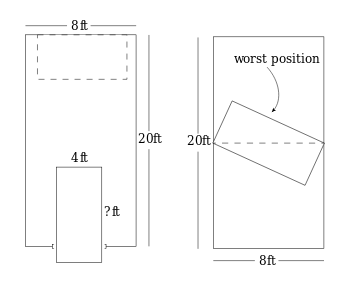
\includegraphics[scale=0.5]{imagens/adventure_g1.png}}
  \end{center}
\end{figure}

\paragraph{G2:} The four-sided solid shown is the part of the solid sphere (of radius 2, centered at the origin) in the first octant. Find its total surface area.

\begin{figure}[H]
  \begin{center}
    %\caption{}
    \label{fig:adv-g2}
    \fbox{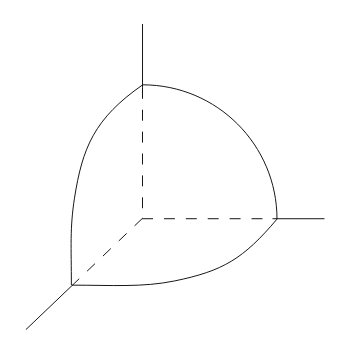
\includegraphics[scale=0.5]{imagens/adventure_g2.png}}
  \end{center}
\end{figure}

\paragraph{G3:} To estimate the height of a skyscraper 1km in the distance, Jenny finds that if her friend Steve stands 2.5 meters away, the top of his head just lines up with the top of the building. Steve is 2 meters tall, and Jenny's eye is 1.5 meters from the ground. How high is the building? (The dotted lines may help you.)

\begin{figure}[H]
  \begin{center}
    %\caption{}
    \label{fig:adv-g3}
    \fbox{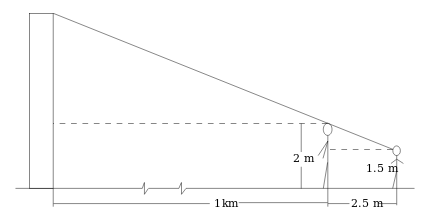
\includegraphics[scale=0.5]{imagens/adventure_g3.png}}
  \end{center}
\end{figure}

%%%%%%%%%%%%%%%%%%%%%%%%%%%%%%%%%%%%%%%%%%%%%%%%%%%%%%%%%%%%%%%%%%%%%%%%%%%%%%%%%
\subsubsection{Trigonometry}
\label{gs-adventure-trigonometry}

\paragraph{T1:} In the given right triangle, what is $\tan{y}$?

\begin{figure}[H]
  \begin{center}
    %\caption{}
    \label{fig:adv-t1}
    \fbox{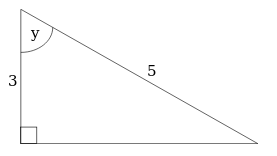
\includegraphics[scale=0.5]{imagens/adventure_t1.png}}
  \end{center}
\end{figure}

\paragraph{T2:} A horse runs counterclockwise (anticlockwise) around the circular track of radius 400m at a constant speed, starting at the marked point. It completes one lap in three minutes. What is its coordinate after one minute? (If needed, you can use ``pi'' for $\pi$, and sqrt(5) for $\sqrt{5}$.)

\begin{figure}[H]
  \begin{center}
    %\caption{}
    \label{fig:adv-t2}
    \fbox{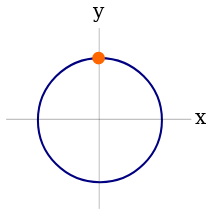
\includegraphics[scale=0.5]{imagens/adventure_t2.png}}
  \end{center}
\end{figure}

\paragraph{T3:} Find the smallest positive solution to the equation $\sin{2x} = \frac{1}{2}$; here $x$ is in radians.
(If needed, you can use ``pi'' for $\pi$, and sqrt(5) for $\sqrt{5}$. You can enter fractions using the forward slash
/ ; e.g. pi/2 for $\frac{\pi}{2}$.)

\paragraph{T4:} A line with slope 1/2 makes an acute angle $\theta$ with the axis. What is $\sin{\theta}$?
(If needed, you can use pi for $\pi$, and sqrt(5) for $\sqrt{5}$. You may enter your answer as a decimal number.)

\paragraph{T5:} By using the trigonometric identity $\cos{2x} = \cos^2{x} - \sin^2{x}$, and other identities,
find the \textbf{positive} expression for $\sin{\left(\frac{A}{2}\right)}$ in terms of $\cos{A}$.

\paragraph{T6:} The graph below represents which of these functions?

\begin{figure}[H]
  \begin{center}
    %\caption{}
    \label{fig:adv-t3}
    \fbox{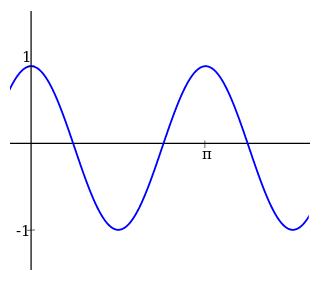
\includegraphics[scale=0.5]{imagens/adventure_t3.png}}
  \end{center}
\end{figure}

\begin{itemize}[noitemsep]
\item[$\square$] $\sin{x}$
\item[$\square$] $\cos{x}$
\item[$\square$] $\sin{(x/2)}$
\item[$\square$] $\cos{(x/2)}$
\item[$\square$] $\sin{2x}$
\item[$\square$] $\cos{2x}$
\end{itemize}

If you got a 0.6 or above, you have the foundational trigonometry understanding to succeed in this course.
Otherwise, you will need to study trigonometry concurrent with this course in order to succeed!

%%%%%%%%%%%%%%%%%%%%%%%%%%%%%%%%%%%%%%%%%%%%%%%%%%%%%%%%%%%%%%%%%%%%%%%%%%%%%%%%%
\subsubsection{Logarithms and exponentials}
\label{gs-adventure-log}

\paragraph{E1:} If $\log_{10}{a}=4.2$ and $\log_{10}{b} = 0.5$, what is $\log_{10}{ab}$?

\paragraph{E2:} If $2^a = \frac{\sqrt{8}}{4^3}$, what is $a$?

\paragraph{E3:} Which of the following is equal to $\sqrt{\frac{x^{16}(1 + x^2)}{9}}$?

\begin{itemize}
\item[$\square$] $\frac{x^4(1+x)}{3}$
\item[$\square$] $\frac{x^8(1+3)}{3}$
\item[$\square$] $\frac{x^4(1+x^2)^{0.5}}{3}$
\item[$\square$] $\frac{x^8(1+x^2)^{0.5}}{3}$
\item[$\square$] $\frac{x^4(1+x^2)}{3}$
\item[$\square$] $\frac{x^8(1+x^2)}{3}$
\item[$\square$] None of the above
\end{itemize}

\paragraph{E4:} Solve for $x$: $\log_{10}\left[(x+1)^2\right] = 2$. (Enter your answer as a list of $x$-values, separated by commas.)

\paragraph{E5:} A pot of water (at sea level) is boiling; the heat is turned off at time $t=0$, and $2$ minutes later the water temperature has fallen to $80$ºC. If the temperature $T$ (in ºC) is expressed in terms of time $t$ (in minutes) by the law

\begin{equation}
  T = Ae^{-kt}
\end{equation}
\noindent
find the values of the constants $A$ and $k$.

If you got a 0.7 or higher, congratulations! You have an excellent understanding of logarithms and exponents! Good work.
You can still succeed in this course if you got a 0.7 or lower, but we strongly recommend that you review logarithms and exponents before you get to the end of Unit 2: Differentiation where logarithms and exponents begin to take on a prominent role in the course.

%%%%%%%%%%%%%%%%%%%%%%%%%%%%%%%%%%%%%%%%%%%%%%%%%%%%%%%%%%%%%%%%%%%%%%%%%%%%%%%%%
\subsubsection{Limits diagnostic}
\label{gs-adventure-limits}

You will NOT see which problems you get correct and incorrect. Sorry if this is frustrating. We will be using these problems to assess whether or not our content teaches you about limits.

\paragraph{L1:} What is $\displaystyle \lim_{x\to\infty} \frac{x^2-4}{2 + x - 4x^2}$?

\begin{itemize}
\item[$\square$] $-2$
\item[$\square$] $-\frac{1}{4}$
\item[$\square$] $\frac{1}{2}$
\item[$\square$] $1$
\item[$\square$] The limit does not exist.
\end{itemize}

\paragraph{L2:} The graph of a function $f$ is shown below. If the limit as $x\to\infty$ exists and $f$ is not continuous at $b$, then $b=$?

\begin{figure}[H]
  \begin{center}
    %\caption{}
    \label{fig:adv-l2}
    \fbox{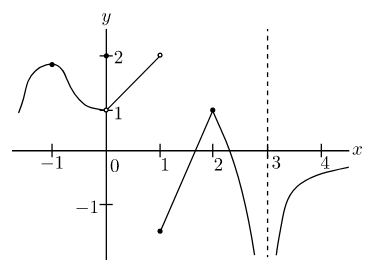
\includegraphics[scale=0.5]{imagens/adventure_l2.png}}
  \end{center}
\end{figure}

\begin{itemize}[noitemsep]
\item[$\square$] $-1$
\item[$\square$] $0$
\item[$\square$] $1$
\item[$\square$] $2$
\item[$\square$] $3$
\end{itemize}

\paragraph{L3:} What is $\displaystyle \lim_{x \to 3} \frac{6/x - 2}{3 -4x + x^2}$? (If the limit does not exist, enter DNE.)

\paragraph{L4:} Which of the following functions have a removable discontinuity at $x=2$?

\begin{itemize}
\item[$\square$] $f(x) = \frac{x^2 - x - 2}{x - 2}$
\item[$\square$] $f(x) = \frac{1}{(x-2)^2}$
\item[$\square$] $f(x) = \begin{cases}
      \frac{x^2 - x - 2}{x-2} & x \ne 2\\
      3                       & x = 2
    \end{cases}$
\item[$\square$] $f(x) = \begin{cases}
      x^3 - 1 & x > 2\\
      -x^2    & x \le 2
    \end{cases}$ 
\end{itemize}

\paragraph{L5:} Identify the left-hand limit $\displaystyle \lim_{x \to -1^-} f(x)$ based on the graph of shown below.

\begin{figure}[H]
  \begin{center}
    %\caption{}
    \label{fig:adv-l5}
    \fbox{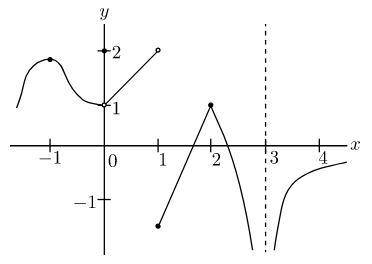
\includegraphics[scale=0.5]{imagens/adventure_l5.png}}
  \end{center}
\end{figure}

\begin{itemize}[noitemsep]
\item[$\square$] $2$
\item[$\square$] $1$
\item[$\square$] $0$
\item[$\square$] $-1$
\item[$\square$] $-1.5$
\item[$\square$] Does not exist.
\end{itemize}

\paragraph{L6:} Identify the right-handed limit $\displaystyle \lim_{x \to -1^+} \frac{x^2 -1}{|x+1|}$.
(Enter DNE if the limit does not exist.)

\begin{itemize}[noitemsep]
\item If you got 0.65 or above, you have a good handle on limits. Move on to Unit 1.
  You can go back to Unit 0 at any time to fill any gaps in your understanding of limits.
\item If you got between .35--.65 points, we recommend that you start by doing the in-lecture
  problems in Unit 0. You may be able to skip the video tutorials.
\item Otherwise, start with Unit 0!
\end{itemize}

%%%%%%%%%%%%%%%%%%%%%%%%%%%%%%%%%%%%%%%%%%%%%%%%%%%%%%%%%%%%%%%%%%%%%%%%%%%%%%%%%
\subsubsection{Derivatives diagnostic}
\label{gs-adventure-derivative}

You will not see which problems you get correct and incorrect. Sorry if this is frustrating. We will be using these problems to assess whether or not our content teaches you about derivatives.

\paragraph{C1:} What is $\displaystyle \lim_{h \to 0} \frac{\cos{(\pi/6 + h)}-\cos{(\pi/6)}}{h}$? 
(Enter the answer as a decimal. If the limit does not exist, enter DNE.)

\paragraph{C2:} At which of the five points on the graph are $\frac{dy}{dx}$ and $\frac{d^2y}{dx^2}$ both negative?

\begin{figure}[H]
  \begin{center}
    %\caption{}
    \label{fig:adv-c2}
    \fbox{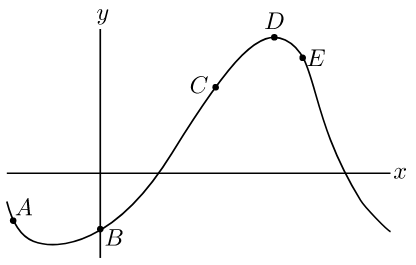
\includegraphics[scale=0.5]{imagens/adventure_c2.png}}
  \end{center}
\end{figure}

\paragraph{C3:} What is the average rate of change of the function $f(x) = x^4 - 5x$ between $x=0$ and $x=3$?

\paragraph{C4:} The position of a particle moving along a line is $p(t) = 2t^3 -24 t^2 +90t + 7$ for $t \ge 0$.
For what values of $t$ is the speed of the particle increasing?

\begin{itemize}[noitemsep]
\item[$\square$] $3 < t < 4$ only
\item[$\square$] $t > 4$ only
\item[$\square$] $t > 5$ only
\item[$\square$] $0 < t < 3$ and $t > 5$
\item[$\square$] $3 < t < 4$ and $t > 5$
\end{itemize}

\paragraph{C5:} Evaluate the limit $\lim_{x \to \infty} \frac{\ln{x}}{x^2}$:

\begin{itemize}[noitemsep]
\item[$\square$] $0$
\item[$\square$] $1$
\item[$\square$] $-1$
\item[$\square$] $\infty$
\item[$\square$] $-\infty$
\end{itemize}

\paragraph{C6:} If $f$ is differentiable at $x=a$, which of the following must be true? Choose all of the following that must be true.

\begin{itemize}[noitemsep]
\item[$\square$] $f$ is continuous at $x=a$.
\item[$\square$] $\lim_{x \to a} f(x)$ exists.
\item[$\square$] $\lim_{x \to a} \frac{f(x) - f(a)}{x-a}$ exists.
\item[$\square$] $f'(a)$ is defined.
\item[$\square$] $f''(a)$ is defined.
\end{itemize}

\paragraph{C7:} Let $f(x)=x^3 + 5x^2 -7x -1$. What is $f'(1)$?

\paragraph{C8:} Let $g(x) = x^2e^x$. What is $g'(1)$?

\paragraph{C9:} Suppose that $f(x) = g(5x)$ for all $x$, and that both functions
are differentiable. Which of the following is necessarily true?

\begin{itemize}[noitemsep]
\item[$\square$] $f'(1) = g'(1)$
\item[$\square$] $f'(5) = g'(1)$
\item[$\square$] $f'(1) = g'(5)$
\item[$\square$] $5f'(1) = g'(1)$
\item[$\square$] $5f'(1) = g'(5)$
\item[$\square$] $f'(1) = 5g'(1)$
\item[$\square$] $f'(1) = 5g'(5)$
\item[$\square$] None of the above.
\end{itemize}

\paragraph{C10:} Let $\displaystyle f(x) = \frac{\ln{(5t+1)}}{\sqrt{t+1}}$. What is $f'(0)$?

If you got 0.8 or above, you have a good handle on the derivative. There is likely no material
in Unit 0 or Unit 1 that you are not familiar with. You may choose to the the
in-lecture exercises, but may wish to skip the video tutorials. If you got less than 0.8, that is to be expected!
We assume you are here to learn about differentiation after all.


%%%%%%%%%%%%%%%%%%%%%%%%%%%%%%%%%%%%%%%%%%%%%%%%%%%%%%%%%%%%%%%%%%%%%%%%%%%%%%%%%
%%%%%%%%%%%%%%%%%%%%%%%%%%%%%%%%%%%%%%%%%%%%%%%%%%%%%%%%%%%%%%%%%%%%%%%%%%%%%%%%%
\subsection{Syllabus and schedule}
\label{gs-syllabus}

%%%%%%%%%%%%%%%%%%%%%%%%%%%%%%%%%%%%%%%%%%%%%%%%%%%%%%%%%%%%%%%%%%%%%%%%%%%%%%%%%
\subsubsection{Syllabus and schedule}
\label{gs-syllabus-syllabus}

\begin{figure}[H]
  \begin{center}
    %\caption{}
    \label{fig:syllabus1}
    \fbox{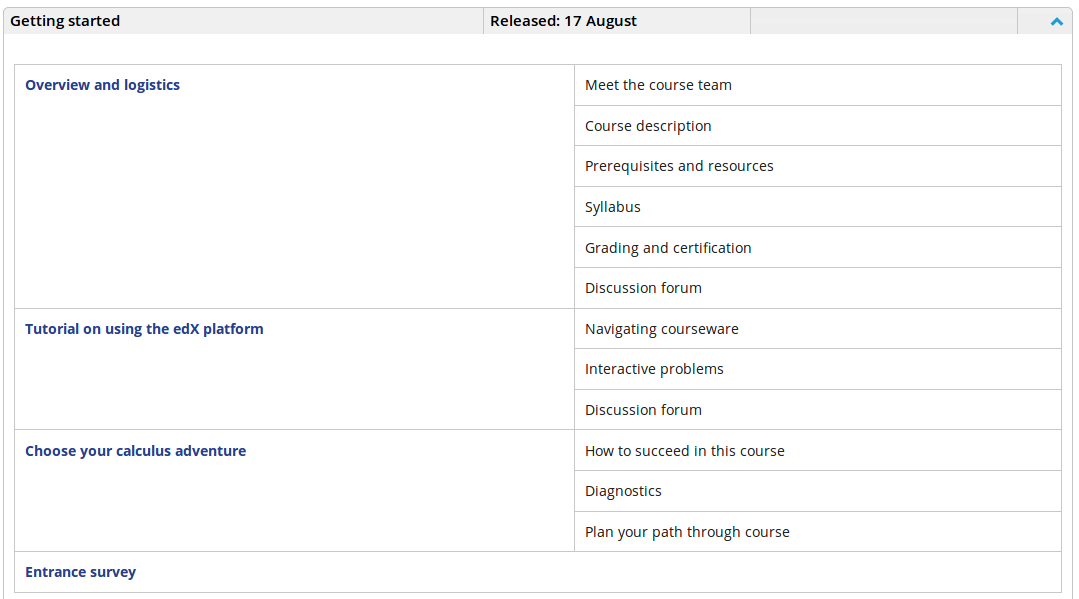
\includegraphics[scale=0.35]{imagens/syllabus1.png}}
  \end{center}
\end{figure}

\begin{figure}[H]
  \begin{center}
    %\caption{}
    \label{fig:syllabus2}
    \fbox{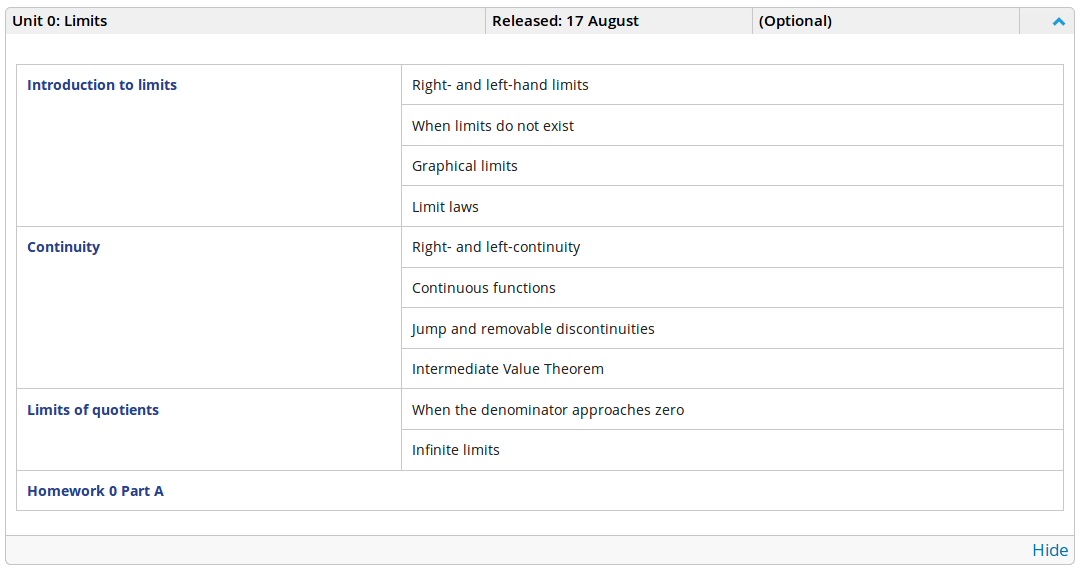
\includegraphics[scale=0.35]{imagens/syllabus2.png}}
  \end{center}
\end{figure}

\begin{figure}[H]
  \begin{center}
    %\caption{}
    \label{fig:syllabus3}
    \fbox{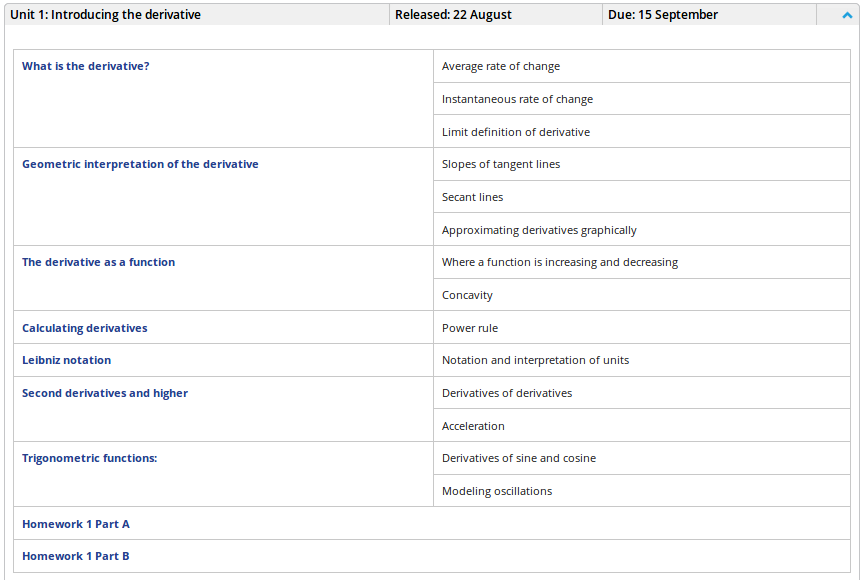
\includegraphics[scale=0.35]{imagens/syllabus3.png}}
  \end{center}
\end{figure}

\begin{figure}[H]
  \begin{center}
    %\caption{}
    \label{fig:syllabus4}
    \fbox{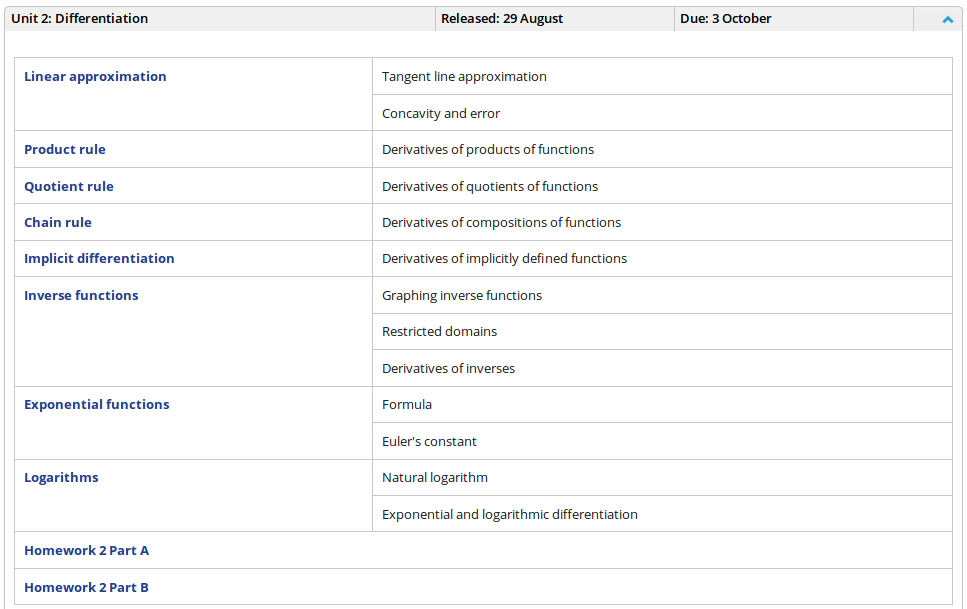
\includegraphics[scale=0.32]{imagens/syllabus4.png}}
  \end{center}
\end{figure}

\begin{figure}[H]
  \begin{center}
    %\caption{}
    \label{fig:syllabus5}
    \fbox{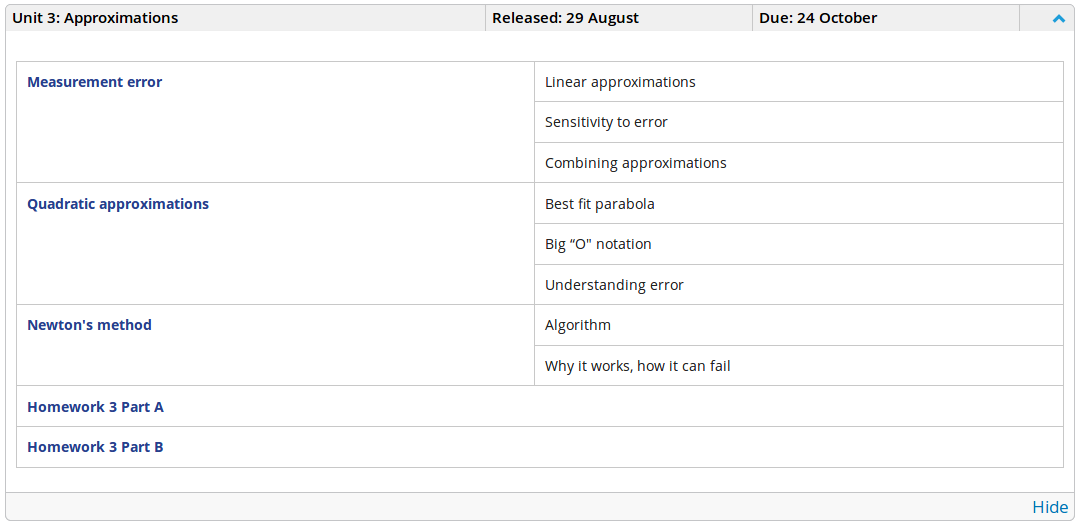
\includegraphics[scale=0.30]{imagens/syllabus5.png}}
  \end{center}
\end{figure}

\begin{figure}[H]
  \begin{center}
    %\caption{}
    \label{fig:syllabus6}
    \fbox{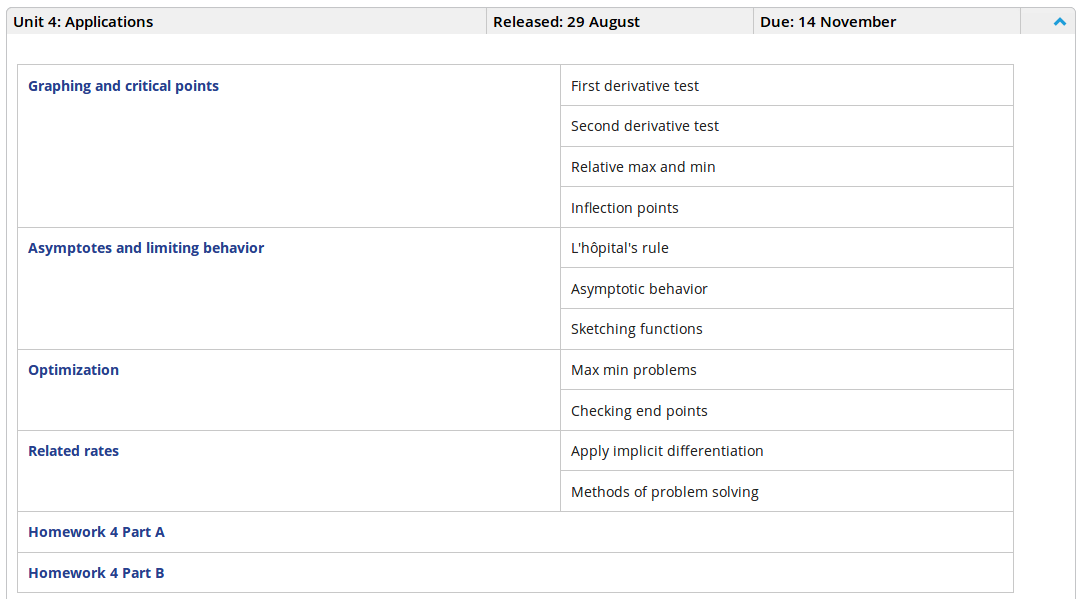
\includegraphics[scale=0.30]{imagens/syllabus6.png}}
  \end{center}
\end{figure}

\begin{figure}[H]
  \begin{center}
    %\caption{}
    \label{fig:syllabus7}
    \fbox{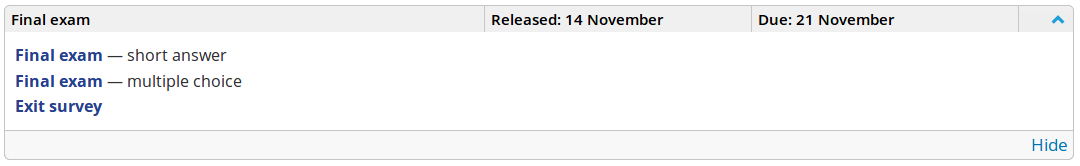
\includegraphics[scale=0.35]{imagens/syllabus7.png}}
  \end{center}
\end{figure}


%%%%%%%%%%%%%%%%%%%%%%%%%%%%%%%%%%%%%%%%%%%%%%%%%%%%%%%%%%%%%%%%%%%%%%%%%%%%%%%%%
%%%%%%%%%%%%%%%%%%%%%%%%%%%%%%%%%%%%%%%%%%%%%%%%%%%%%%%%%%%%%%%%%%%%%%%%%%%%%%%%%
\subsection{Entrance survey}
\label{gs-survey}

%%%%%%%%%%%%%%%%%%%%%%%%%%%%%%%%%%%%%%%%%%%%%%%%%%%%%%%%%%%%%%%%%%%%%%%%%%%%%%%%%
\subsubsection{Entrance survey}
\label{gs-survey-survey}

Welcome to this online course from MITx.

For us to offer the best course experience possible, we'd like to ask you to answer a few questions about yourself.

Whether you are just browsing or you are determined to complete the entire course, the more we know about you, the better we can serve all students in this course. As one of the first students in this new, free offering, your responses will be especially important to us. 

There are no right or wrong answers or responses, and your honest feedback is very important to us.  After reading the consent document below, you may click the right arrow below to proceed. 

\textbf{General Information About Survey Research in MITx. Please Read then Click Below to Continue.}

\textbf{Participation is voluntary}.
All survey responses are voluntary, students can skip any question at any time, and any responses have no effect on student assessments or participation. 

\textbf{What is the purpose of this research?}
We are interested in learning more about our participants’ backgrounds, interests, and motivations, and encouraging engagement with the course, so we can do the best possible job designing, evaluating and refining this course. With this research we will understand how to best encourage engagement with online education . 

\textbf{How long will I take part in this research?}
Your participation will be the duration of the course.

\textbf{What can I expect if I take part in this research?}
As a participant, you will be provided questions about yourself and other short prompts, which we will use to understand your participation in the course.  
 
\textbf{What are the risks and possible discomforts?}
If you choose to participate, we anticipate minimal risks and only the minor discomfort that might accompany online surveys. 

\textbf{Are there any benefits from being in this research study? }
We cannot promise any benefits to you or others from taking part in this research. However, possible benefits include your being more engaged with the course and better serving future students who participate in online courses. 

\textbf{If I take part in this research, how will my privacy be protected? What happens to the information you collect?}
Your instructor will not be able to identify your personal responses during the course and researchers will not attempt to identify individuals.  Your data will not be made identifiable to anyone other than researchers and course staff, and it will be aggregated for analysis and publication purposes. 

\textbf{If I have any questions, concerns or complaints about this research study, who can I talk to?}
The researcher for this study is Justin Reich who can be reached at 617-715-2962, 600 Technology Square, NE49-2028, Cambridge, MA, 02139, jreich@mit.edu for any of the following:
\begin{itemize}
\item If you have questions, concerns, or complaints,
\item If you would like to talk to the research team,
\item If you think the research has harmed you, or
\item If you wish to withdraw from the study.
\end{itemize}

This research has been reviewed by the Committee on the Use of Human Subjects in Research at Harvard University.  They can be reached at 617-496-2847, 1414 Massachusetts Avenue, Second Floor, Cambridge, MA 02138, or cuhs@fas.harvard.edu for any of the following:
\begin{itemize}
\item If your questions, concerns, or complaints are not being answered by the research team,
\item If you cannot reach the research team,
\item If you want to talk to someone besides the research team, or
\item If you have questions about your rights as a research participant.
\end{itemize}

Please print or save a copy of this form for your records.
\textbf{If you agree to participate, please click "Next" to enter the survey.}

\begin{figure}[H]
  \begin{center}
    %\caption{}
    \label{fig:survey01}
    \fbox{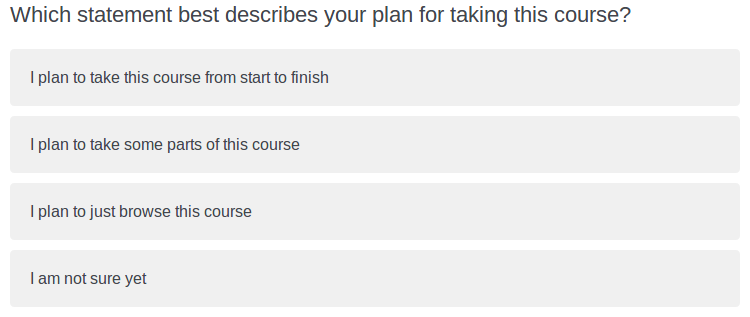
\includegraphics[scale=0.5]{imagens/survey01.png}}
  \end{center}
\end{figure}

\begin{figure}[H]
  \begin{center}
    %\caption{}
    \label{fig:survey02}
    \fbox{
\includegraphics[scale=0.5]{imagens/survey02.png}}
  \end{center}
\end{figure}

\begin{figure}[H]
  \begin{center}
    %\caption{}
    \label{fig:survey03}
    \fbox{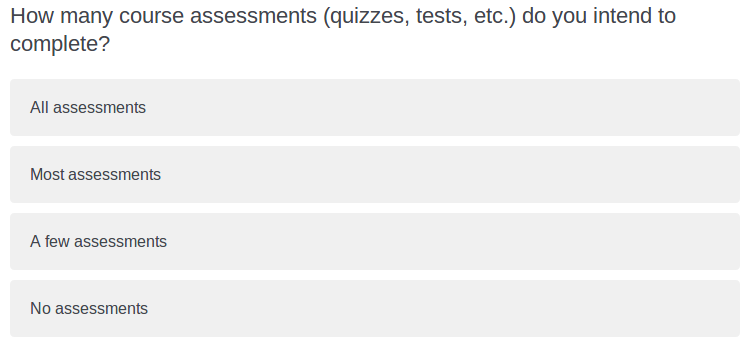
\includegraphics[scale=0.5]{imagens/survey03.png}}
  \end{center}
\end{figure}

\begin{figure}[H]
  \begin{center}
    %\caption{}
    \label{fig:survey04}
    \fbox{
\includegraphics[scale=0.5]{imagens/survey04.png}}
  \end{center}
\end{figure}

\begin{figure}[H]
  \begin{center}
    %\caption{}
    \label{fig:survey05}
    \fbox{
\includegraphics[scale=0.5]{imagens/survey05.png}}
  \end{center}
\end{figure}

\begin{figure}[H]
  \begin{center}
    %\caption{}
    \label{fig:survey06}
    \fbox{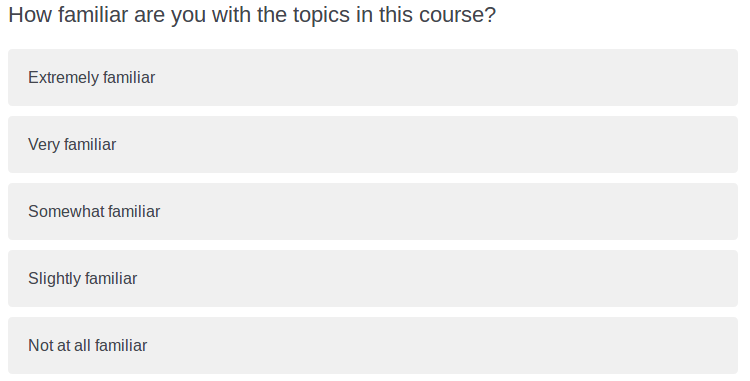
\includegraphics[scale=0.5]{imagens/survey06.png}}
  \end{center}
\end{figure}

\begin{figure}[H]
  \begin{center}
    %\caption{}
    \label{fig:survey07}
    \fbox{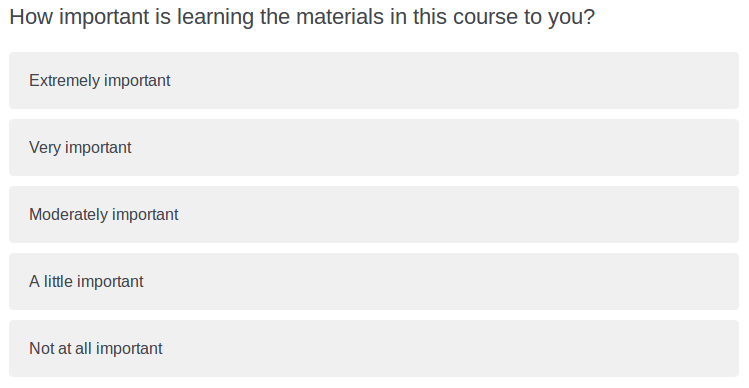
\includegraphics[scale=0.5]{imagens/survey07.png}}
  \end{center}
\end{figure}

\begin{figure}[H]
  \begin{center}
    %\caption{}
    \label{fig:survey08}
    \fbox{
\includegraphics[scale=0.5]{imagens/survey08.png}}
  \end{center}
\end{figure}

\begin{figure}[H]
  \begin{center}
    %\caption{}
    \label{fig:survey09}
    \fbox{
\includegraphics[scale=0.5]{imagens/survey09.png}}
  \end{center}
\end{figure}

\begin{figure}[H]
  \begin{center}
    %\caption{}
    \label{fig:survey10}
    \fbox{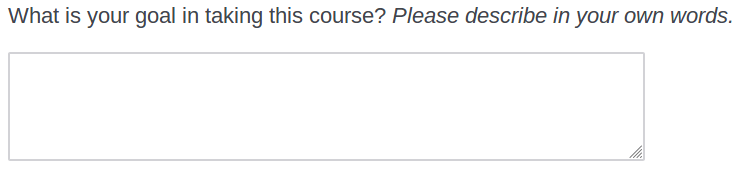
\includegraphics[scale=0.5]{imagens/survey10.png}}
  \end{center}
\end{figure}

\begin{figure}[H]
  \begin{center}
    %\caption{}
    \label{fig:survey11}
    \fbox{
\includegraphics[scale=0.5]{imagens/survey11.png}}
  \end{center}
\end{figure}

\begin{figure}[H]
  \begin{center}
    %\caption{}
    \label{fig:survey12}
    \fbox{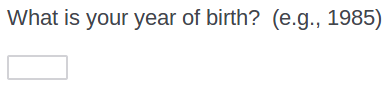
\includegraphics[scale=0.5]{imagens/survey12.png}}
  \end{center}
\end{figure}

\begin{figure}[H]
  \begin{center}
    %\caption{}
    \label{fig:survey13}
    \fbox{
\includegraphics[scale=0.5]{imagens/survey13.png}}
  \end{center}
\end{figure}

\begin{figure}[H]
  \begin{center}
    %\caption{}
    \label{fig:survey14}
    \fbox{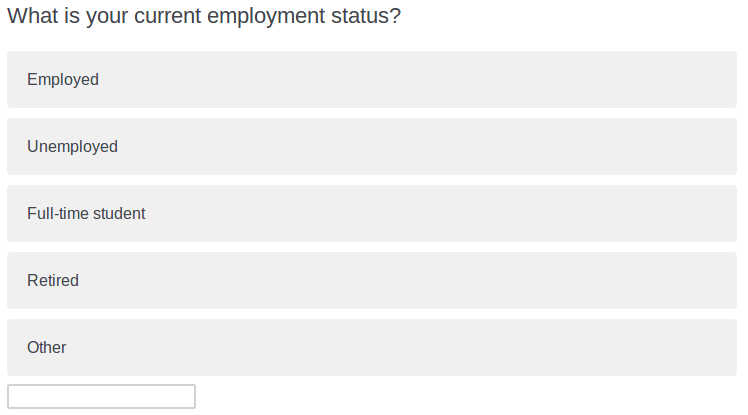
\includegraphics[scale=0.5]{imagens/survey14.png}}
  \end{center}
\end{figure}

\begin{figure}[H]
  \begin{center}
    %\caption{}
    \label{fig:survey15}
    \fbox{
\includegraphics[scale=0.5]{imagens/survey15.png}}
  \end{center}
\end{figure}

\begin{figure}[H]
  \begin{center}
    %\caption{}
    \label{fig:survey16}
    \fbox{
\includegraphics[scale=0.5]{imagens/survey16.png}}
  \end{center}
\end{figure}

\begin{figure}[H]
  \begin{center}
    %\caption{}
    \label{fig:survey17}
    \fbox{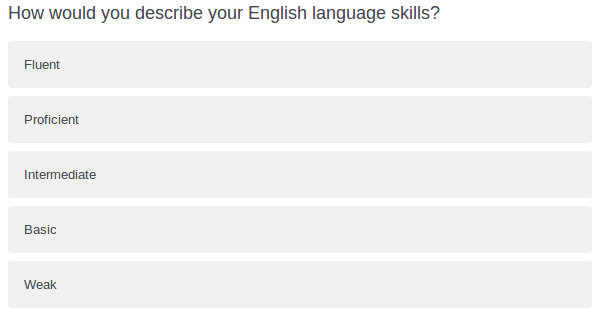
\includegraphics[scale=0.5]{imagens/survey17.png}}
  \end{center}
\end{figure}

\begin{figure}[H]
  \begin{center}
    %\caption{}
    \label{fig:survey18}
    \fbox{
\includegraphics[scale=0.5]{imagens/survey18.png}}
  \end{center}
\end{figure}

\begin{figure}[H]
  \begin{center}
    %\caption{}
    \label{fig:survey19}
    \fbox{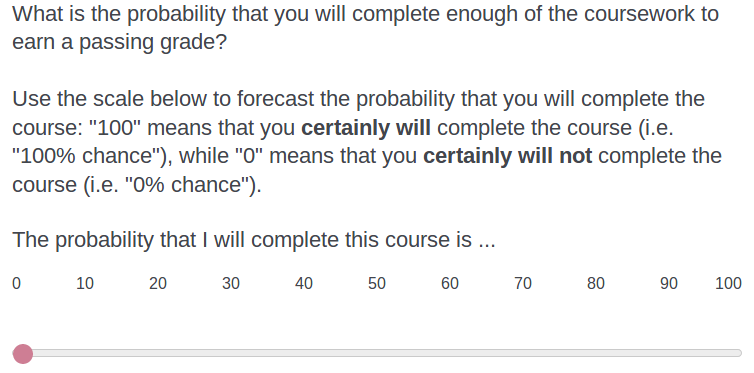
\includegraphics[scale=0.5]{imagens/survey19.png}}
  \end{center}
\end{figure}

\begin{figure}[H]
  \begin{center}
    %\caption{}
    \label{fig:survey20}
    \fbox{
\includegraphics[scale=0.5]{imagens/survey20.png}}
  \end{center}
\end{figure}

\begin{figure}[H]
  \begin{center}
    %\caption{}
    \label{fig:survey21}
    \fbox{
\includegraphics[scale=0.5]{imagens/survey21.png}}
  \end{center}
\end{figure}

\begin{figure}[H]
  \begin{center}
    %\caption{}
    \label{fig:survey22}
    \fbox{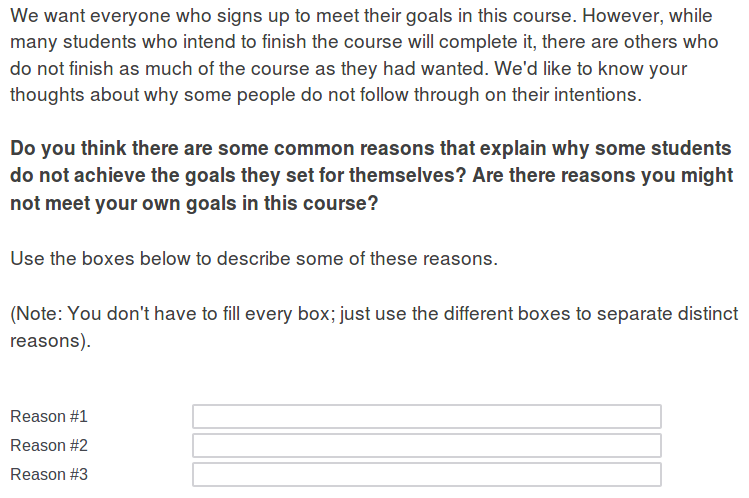
\includegraphics[scale=0.5]{imagens/survey22.png}}
  \end{center}
\end{figure}

\begin{figure}[H]
  \begin{center}
    %\caption{}
    \label{fig:survey23}
    \fbox{
\includegraphics[scale=0.5]{imagens/survey23.png}}
  \end{center}
\end{figure}

\begin{figure}[H]
  \begin{center}
    %\caption{}
    \label{fig:survey24}
    \fbox{
\includegraphics[scale=0.5]{imagens/survey24.png}}
  \end{center}
\end{figure}

\begin{figure}[H]
  \begin{center}
    %\caption{}
    \label{fig:survey25}
    \fbox{
\includegraphics[scale=0.5]{imagens/survey25.png}}
  \end{center}
\end{figure}

\begin{figure}[H]
  \begin{center}
    %\caption{}
    \label{fig:survey26}
    \fbox{
\includegraphics[scale=0.5]{imagens/survey26.png}}
  \end{center}
\end{figure}




%%%%%%%%%%%%%%%%%%%%%%%%%%%%%%%%%%%%%%%%%%%%%%%%%%%%%%%%%%%%%%%%%%%%%%%%%%%%%%%%%
%%%%%%%%%%%%%%%%%%%%%%%%%%%%%%%%%%%%%%%%%%%%%%%%%%%%%%%%%%%%%%%%%%%%%%%%%%%%%%%%%
%%%%%%%%%%%%%%%%%%%%%%%%%%%%%%%%%%%%%%%%%%%%%%%%%%%%%%%%%%%%%%%%%%%%%%%%%%%%%%%%%
\newpage
\section{Unit 0: limits}
\label{u0}


%%%%%%%%%%%%%%%%%%%%%%%%%%%%%%%%%%%%%%%%%%%%%%%%%%%%%%%%%%%%%%%%%%%%%%%%%%%%%%%%%
%%%%%%%%%%%%%%%%%%%%%%%%%%%%%%%%%%%%%%%%%%%%%%%%%%%%%%%%%%%%%%%%%%%%%%%%%%%%%%%%%
\subsection{Introduction to limits}
\label{u0-intro}

%%%%%%%%%%%%%%%%%%%%%%%%%%%%%%%%%%%%%%%%%%%%%%%%%%%%%%%%%%%%%%%%%%%%%%%%%%%%%%%%%
\subsubsection{Motivation}
\label{u0-intro-motiv}

Video: \href{https://www.youtube.com/watch?v=nh5O6-2Evk8}{Introduction to Limits}

Calculus has two main concepts --- the \emph{derivative}
and the \emph{integral}.
But in order to understand either of them,
you first have to understand limits.

So let's talk limits.
We'll start with a curve.
Fix a point $A$ on the curve.
Choose a second point, $B$, which we're going to move.
And draw a line through $A$ and $B$. Let's look
at what happens when $B$ moves closer and closer to the point
$A$.

This is an example of a limit.
In the limit, the line becomes tangent to the curve
at the point $A$. The slope of this line
is the derivative at the point $A$.

Now let's see how limits
are related to integrals.
Integrals are used to measure areas of curvy regions
like this.

Measuring areas of curvy regions seems hard,
but measuring areas of rectangles
is easy, so we'll try to fill our region with rectangles.

Each rectangle has a certain width.
As we make the width smaller, the total area
of the rectangles gets closer and closer
to the area of the curvy region.
The integral is the limit of the total area of the rectangles
as the width tends to zero.

So that's why we start with limits.
They're the foundation for everything else in calculus.
At the beginning, limits may seem abstract,
but very quickly you'll get used to them.

%%%%%%%%%%%%%%%%%%%%%%%%%%%%%%%%%%%%%%%%%%%%%%%%%%%%%%%%%%%%%%%%%%%%%%%%%%%%%%%%%
\subsubsection{Introduction to limits}
\label{u0-intro-intro}

\paragraph{Objectives} At the end of this sequence, and after some practice, you should be able to:
\begin{itemize}[noitemsep]
\item Use a calculator to determine right and left hand limits.
\item Identify right and left hand limits based on graphs.
\item Determine if a limit exists based on values of right and left hand limits.
\item Understand that the limit does not depend on the value of a function at the point of interest.
\end{itemize}

Contents: 14 pages, 6 videos (24 minutes 1x speed), 17 questions.

%%%%%%%%%%%%%%%%%%%%%%%%%%%%%%%%%%%%%%%%%%%%%%%%%%%%%%%%%%%%%%%%%%%%%%%%%%%%%%%%%
\subsubsection{Moving closer and closer}
\label{u0-intro-moving}

Video: \href{https://www.youtube.com/watch?v=bANtYKLugsU}{Moving closer and closer}

Welcome.

Calculus is all about functions. You probably know that a function $f$ takes an input $x$
and gives an output $f(x)$. But in calculus, we're not concerned with just one input
and finding the output for that one input. We want to consider a whole range of inputs.
So we would want to know what happens when the input ``moves'' or ``varies''.
For instance, we could ask what happens as the input moves really close.
Closer and closer to some point. Let's say $1$.

And to be even more specific, let's say that $x$ is moving towards $1$ from the left.
So if this is a number line, and we've got the point $1$ right there, then $x$
could start here, and just move closer and closer and closer towards $1$, from the left.
We'll use this arrow notation ($x \to 1^{-}$) to denote that $x$ is getting really, really close to $1$,
from the left.
But a warning, this does not mean that \emph{$x$ will ever actually equal $1$}.
We're only concerned with values of $x$ that are \emph{near} one.

OK. Now that that's said, as $x$ moves,
we know that the output $f(x)$ is also going to move.
And so the question that we can ask
is as $x$ moves closer and closer to $1$ from the left,
does $f(x)$ move closer and closer
to some value of its own?

Let's be concrete here.
And pick a particular function $f$.
I'm going to choose $\displaystyle f(x) = \frac{\sqrt{3-5x+x^2+x^3}}{x-1}$.
Kind of a complicated function, but you'll
have to trust me that this is a good example.

And what we can do in order to see what's
happening to $f$ as $x \to 1^{-}$,
is just select certain values of $x$
that are getting closer and closer to $1$ from the left.
So over here on the number line, we
could start with $x$ equals zero.
And then they get closer, we could try x equals $0.5$.
Or even closer, maybe $0.9$.
Even $0.99$.
These sorts of values.
And we want to know, what's happening to the output?
So we can just plug these values into the function,
and see whether the output gets closer and closer to anything.

Now there are technically infinitely many values
of $x$ that we could have chosen here.
But let's just start with these four.
Remember though that one value of $x$
that we will definitely not consider
is $x = 1$ itself.
In fact, this function isn't even defined at $x = 1$.
We'd have a zero denominator.
It is, however, defined when $x$ is approaching one,
and those are the values we're considering.

OK.
Well let's make a table with our chosen
inputs and the associated outputs,
and let's just calculate those outputs.
So when we plug in zero we'll get a square root of 3
on top divided by minus 1.
So minus square root of 3, which is roughly minus $1.73$.

Next up is x equals 0.5.
I'm going to have to bust out the calculator here.
So we've got 3 minus 5 times 0.5 plus 0.5 squared
plus 0.5 cubed, and then we need the square root,
and then we need to divide by 0.5 minus 1.
So 0.5 negative.
So we get minus $1.87$, roughly.

So back to our table.
We've got f of x moving from minus 1.73 to minus 1.87.
Well that's not really enough data
to tell if f is getting closer and closer to anything
in particular.
So let's take our next two values of x and plug those in.
I'm going to fast forward through the calculations.
You ready?

x equals 0.9.
All right?
That's approximately minus 1.97, and finally 0.99,
and we've got minus 1.997.

So as we go down this table, $f(x)$
is getting really, really close to what looks like minus 2.
So we can say that as $x$ approaches $1$ from the left,
$f(x)$ approaches minus 2.

Now $f(x)$ might \emph{never actually equal to $-2$},
just as $x$ never actually equals one,
but it gets really, really close.
And if it gets arbitrarily close,
meaning as close as we could possibly want,
then that's really all we'll care about.

What I would like you to do now is
to do this same exercise, except this time have $x$ approach $1$
from the right. You might be surprised at what you find.
We'll talk afterwards.

\begin{exercise}
  Determine what happens to $\displaystyle f(x) = \frac{\sqrt{3-5x+x^2+x^3}}{x-1}$
  as $x$ approaches $1$ from the right. Take values of $x$ that are greater than 1,
  but getting closer and closer to 1. For instance, you could try
  $x=1.1, 1.01, 1.001, 1.0001$, etc. What happens to $f(x)$ as $x$ approaches
  1 from the right?
\begin{itemize}[noitemsep]
\item[$\square$] $f(x)$ gets closer and closer to a particular number
\item[$\square$] $f(x)$ gets bigger and bigger in the positive direction without bound
\item[$\square$] $f(x)$ gets bigger and bigger in the negative direction without bound
\item[$\square$] None of the above
\end{itemize}
\end{exercise}

\begin{exercise}
  What value does $f(x)$ get closer to? Enter the number below;
  if there is no such value, enter capital DNE (for "does not exist")
\end{exercise}

%%%%%%%%%%%%%%%%%%%%%%%%%%%%%%%%%%%%%%%%%%%%%%%%%%%%%%%%%%%%%%%%%%%%%%%%%%%%%%%%%
\subsubsection{One-sided limits}
\label{u0-intro-one-sided}

Video: \href{https://www.youtube.com/watch?v=fAAzAVHVKQk}{One-sided limits}

Welcome back.
We've been thinking about this function.
And in the last video, we took some values
of $x$ that were approaching $1$ from the left ($x \to 1^{-}$),
and we made this table.
And we saw that as $x$ approached $1$
from the left, $f(x)$ approached $-2$.
So remember, these arrows mean approaching.
And this minus sign up here, that
signifies that we're coming at $1$ from the left,
or from the negative direction.
This is not the same as $-1$.
$x$ is actually approaching positive $1$.
It's just that $x$ is coming from the negative direction.
And as it does that, $f(x) \to -2$.

What you were supposed to do was the same thing,
just on the other side.
So you should have picked out some values and made a table.
Now, you didn't have to choose these particular values.
But you should have chosen some similar looking ones
and gotten a similar looking table.
And what we see from the table is
that as $x \to 1^{+}$,
$f(x) \to 2$, positive $+2$, not negative $-2$.
So we've got something different going on on the right side of $1$
versus the left side of $1$.
Pretty cool.

\begin{figure}[H]
  \begin{center}
    %\caption{}
    \label{fig:one-sided-limits-1}
    \fbox{\includegraphics[scale=0.5]{imagens/unit-0/limit_001.png}}
  \end{center}
\end{figure}

Let's see what this looks like on the graph of $f$.
All of these data points that we have will help us get started.
For instance, on the right here, we've got $f(2) = 2.24$.
So the point $(2, 2.24)$ is on the graph.
And we can do the same thing with these other three points
that are on the right.
And they'll look like this.

Now, it seems reasonable to assume that the graph of $f$
is going to behave pretty smoothly in between these four
points.
So we can just draw it like this.
And once we've done that, then we can look and see
what happens as $x \to 1^{+}$, what's
happening to $f(x)$ and what's happening to these $y$ values.
Well, like we said, they're approaching
the level $y = 2$.

What happens exactly at $x = 1$?
Well, remember that $f(1)$ isn't defined.
We would have had a $0$ denominator, which
means that there is no point on the graph where
the x-coordinate is $1$.
So we're going to put this open circle here
to remind us that this point, $(1,2)$
is not actually on the graph.
But that's OK.
If we're just talking about $x \to 1$,
that means we only care about values of $x$ that are \emph{near} $1$,
\emph{not equal} to $1$.

We can do the same thing on the left.
Our table of values gives us these four points.
And if we interpolate and assume the graph
is smooth in between those points, then we've got this.
And as we come in towards $1$ from the left with our $x$ values,
then our $y$ values are approaching $y = -2$.
And again, we'll have this open circle
to remind us that there is no point at $x = 1$
on the graph.

\begin{figure}[H]
  \begin{center}
    %\caption{}
    \label{fig:one-sided-limits-2}
    \fbox{\includegraphics[scale=0.5]{imagens/unit-0/limit_002.png}}
  \end{center}
\end{figure}

OK, let me make some space here.
And we want to give an official name
for this phenomenon of a \emph{function's value
approaching something}.
We're going to call this a \emph{limit}.

So on the right here, we're going
to say that the limit of $f(x)$ as $x \to 1^{+}$
is $2$.
And the notation for this is as follows:
$\displaystyle \lim_{x \to 1^{+}} f(x) = 2$.
This is often called the \emph{right-sided} limit
or the right-hand limit \emph{at the point $x = 1$}.
And we have a similar thing on the left.
We can write $\displaystyle \lim_{x \to 1^{-}} f(x) = -2$.

\begin{figure}[H]
  \begin{center}
    %\caption{}
    \label{fig:one-sided-limits-3}
    \fbox{\includegraphics[scale=0.5]{imagens/unit-0/limit_003.png}}
  \end{center}
\end{figure}

And there we have it.
We've got our left-hand limit, and we've
got our right-hand limit.
We have the notation, we have the meaning,
and we know what it looks like in pictures.
So this is our left-handed limit.
And here's our right-handed limit.
So that's our first function.
Kind of an interesting little function, isn't it?
We have a couple short questions for you.
And then we have a few more functions for you
to play around with left- and right-hand limits.
And maybe those will be even more interesting.
So why don't you go and find out?

%%%%%%%%%%%%%%%%%%%%%%%%%%%%%%%%%%%%%%%%%%%%%%%%%%%%%%%%%%%%%%%%%%%%%%%%%%%%%%%%%
\subsubsection{Definitions of right-hand and left-hand limits}
\label{u0-intro-right-left}

\begin{figure}[H]
  \begin{center}
    %\caption{}
    \label{fig:one-sided-limits-4}
    \fbox{\includegraphics[scale=0.5]{imagens/unit-0/limit_004.png}}
  \end{center}
\end{figure}

Suppose $f(x)$ gets really close to $R$ for values of $x$ that get really
close to (but are not equal to) $a$ from the right. Then we say $R$ is the
\emph{right-hand limit} of the function $f(x)$ as $x$ approaches $a$ from the right.
We write

\begin{equation}
  \begin{split}
    f(x) \to R \text{ as } x \to a^{+}\\
    \text{ or }\\
    \lim_{x \to a^{+}} f(x) = R
  \end{split}
\end{equation}

If $f(x)$ gets really close to $L$ for values of $x$ that get really
close to (but are not equal to) $a$ from the left, then we say $L$ is the
\emph{left-hand limit} of the function $f(x)$ as $x$ approaches $a$ from the left.
We write

\begin{equation}
  \begin{split}
    f(x) \to L \text{ as } x \to a^{-}\\
    \text{ or }\\
    \lim_{x \to a^{-}} f(x) = L
  \end{split}
\end{equation}

%%%%%%%%%%%%%%%%%%%%%%%%%%%%%%%%%%%%%%%%%%%%%%%%%%%%%%%%%%%%%%%%%%%%%%%%%%%%%%%%%
\subsubsection{A few more limits}
\label{u0-intro-more}

\begin{exercise}
  \textbf{Another function:} Let's explore the right and left hand limits of a
  few more functions. In this problem, we'll examine the function
  $\displaystyle g(x) = \frac{x}{\tan{(2x)}}$ as $x \to 0$.
  Here is a table of values of $g(x)$ as $x \to 0^{+}$:
  \begin{figure}[H]
  \begin{center}
    %\caption{}
    %\label{fig:}
    \fbox{\includegraphics[scale=0.5]{imagens/unit-0/limit_005.png}}
  \end{center}
  \end{figure}
  Use the calculator to find the left-hand limit (calculator in radians!).
  \begin{itemize}[noitemsep]
  \item[$\square$] As $x \to 0^{-}$, $g(x)$ gets closer and closer to a particular number $L$
    ($g(x) \to L$)
  \item[$\square$] As $x \to 0^{-}$, $g(x)$ gets bigger and bigger without bound
    ($g(x) \to +\infty$)
\item[$\square$] As $x \to 0^{-}$, $g(x)$ gets bigger and bigger in the negative direction without bound
    ($g(x) \to -\infty$)  
\item[$\square$] As $x \to 0^{-}$, $g(x)$ approaches neither a finite number $L$, nor $+\infty$,
  nor $-\infty$
  \end{itemize}
\end{exercise}

\begin{exercise}
  What value does $g(x)$ get closer to as $x \to 0^{-}$? (If it approaches a finite
  number, enter the number below; in any other case, enter capital DNE for "does not exist".)
\end{exercise}

\begin{exercise}
  \textbf{Yet another function:} In this problem, we we'll examine the function
  $\displaystyle h(x) = \frac{|x| + \sin{(x)}}{x^2}$, as $x \to 0$.
  Here is a table of values of $g(x)$ as $x \to 0^{-}$:
  \begin{figure}[H]
  \begin{center}
    %\caption{}
    %\label{fig:}
    \fbox{\includegraphics[scale=0.5]{imagens/unit-0/limit_006.png}}
  \end{center}
  \end{figure}
  Use the calculator to find the right-hand limit (calculator in radians!).
  \begin{itemize}[noitemsep]
  \item[$\square$] As $x \to 0^{+}$, $h(x)$ gets closer and closer to a particular number $R$
    ($h(x) \to R$)
  \item[$\square$] As $x \to 0^{+}$, $h(x)$ gets bigger and bigger without bound
    ($h(x) \to +\infty$)
\item[$\square$] As $x \to 0^{+}$, $h(x)$ gets bigger and bigger in the negative direction without bound
    ($h(x) \to -\infty$)  
\item[$\square$] As $x \to 0^{+}$, $h(x)$ approaches neither a finite number $R$, nor $+\infty$,
  nor $-\infty$
  \end{itemize}
\end{exercise}

\begin{exercise}
  What value does $h(x)$ get closer to as $x \to 0^{+}$? (If it approaches a finite
  number, enter the number below; in any other case, enter capital DNE for "does not exist".)
\end{exercise}

\begin{exercise}
  \textbf{One last function:} In this problem, we we'll examine the function
  $\displaystyle j(x) = \sin{\left(\frac{13}{x}\right)}$, as $x \to 0^{+}$. Use a
  calculator to figure out what $\displaystyle \lim_{x \to 0^{+}} j(x)$ might be.
  Make sure your calculator is in radians!
    \begin{itemize}[noitemsep]
  \item[$\square$] As $x \to 0^{+}$, $j(x)$ gets closer and closer to a particular number $R$
    ($j(x) \to R$)
  \item[$\square$] As $x \to 0^{+}$, $j(x)$ gets bigger and bigger without bound
    ($j(x) \to +\infty$)
\item[$\square$] As $x \to 0^{+}$, $j(x)$ gets bigger and bigger in the negative direction without bound
    ($j(x) \to -\infty$)  
\item[$\square$] As $x \to 0^{+}$, $j(x)$ approaches neither a finite number $R$, nor $+\infty$,
  nor $-\infty$
  \end{itemize}
\end{exercise}

\begin{exercise}
  What value does $j(x)$ get closer to as $x \to 0^{+}$? (If it approaches a finite
  number, enter the number below; in any other case, enter capital DNE for "does not exist".)
\end{exercise}
  

%%%%%%%%%%%%%%%%%%%%%%%%%%%%%%%%%%%%%%%%%%%%%%%%%%%%%%%%%%%%%%%%%%%%%%%%%%%%%%%%%
\subsubsection{Possible limits behaviors}
\label{u0-intro-behaviors}

Video: \href{https://www.youtube.com/watch?v=LCdQyNilFn8}{Possible limits behaviors}

You've now seen a variety of limits.
In our last video, we looked at a function $f$
whose limit as $x$ approached a point a from the right
was equal to $2$.
And so it looked something like this.
And the limit from the left as x approached a was minus 2.
So it looked something like this.
So we know that the right- and the left-hand limits at a point
don't have to agree, but they could agree.

\begin{figure}[H]
  \begin{center}
    %\caption{}
    %\label{fig:}
    \fbox{\includegraphics[scale=0.4]{imagens/unit-0/limit_007.png}}
  \end{center}
\end{figure}

One of the examples that you looked at was like that.
That was the function that we called $g$.
There we had the left-hand limit equal to $1/2$.
So the graph would look like this.
And the right-hand limit was also equal to $1/2$.
So the graph would look something like that.

\begin{figure}[H]
  \begin{center}
    %\caption{}
    %\label{fig:}
    \fbox{\includegraphics[scale=0.4]{imagens/unit-0/limit_008.png}}
  \end{center}
\end{figure}

Now, of course, for the purposes of limits,
it wouldn't have mattered what $g(a)$ itself was.
$g(a)$ could of been down here or it
could've been equal to the value of the limit in which case
we would have had a dot up here.
For the actual function, I think $g(a)$ didn't exist at all,
but that's OK.
That's the great thing about limits,
which is that if you have a formula or a function that
doesn't exist or doesn't work when you try
to plug in some value $a$, you can still say something
about \emph{how it behaves near $a$ by taking limits}.

But sometimes the limits themselves don't exist.
So you saw another function $h$ where
as $x$ approached point $a$ from the left,
the limit was perfectly fine.
And I think, it was 0, but coming in from the right
the value of the function just kept
getting bigger, and bigger, and bigger without bound.
So its graph would have had this sort of vertical asymptote
as we come in from that side towards $a$.
So in this case, when $h$ doesn't approach any particular value
coming in from the side, we say that the limit does not exist.
And we'll always write DNE for does not exist.
So that's one way in which a one-sided limit might not
exist.

\begin{figure}[H]
  \begin{center}
    %\caption{}
    %\label{fig:}
    \fbox{\includegraphics[scale=0.4]{imagens/unit-0/limit_009.png}}
  \end{center}
\end{figure}

The function just kind of blows up towards infinity as we
come in from one side.
Of course, we could have had $h$ going the other way.
It could have blown up towards minus infinity
and that would also be a limit that doesn't exist.

\begin{figure}[H]
  \begin{center}
    %\caption{}
    %\label{fig:}
    \fbox{\includegraphics[scale=0.44]{imagens/unit-0/limit_010.png}}
  \end{center}
\end{figure}

But in the last function that we gave you, which we called $j$,
was something that was even more bizarre.
So there we had a function and it didn't get very big,
either positive nor negative.
In fact, I don't know if you noticed,
but it was always between the values $y = 1$
and $y = -1$, but it never settled down.
As $x$ was coming in towards the value,
hopefully, you saw that $j(x)$ just
kept bouncing back and forth, going up and down, faster
and faster, until it just kind of goes haywire as $x$ comes in
really, really close to $a$.

\begin{figure}[H]
  \begin{center}
    %\caption{}
    %\label{fig:}
    \fbox{\includegraphics[scale=0.5]{imagens/unit-0/limit_011.png}}
  \end{center}
\end{figure}

So, yeah, really weird.
We'll try not to give you too many functions like this,
but you should be aware that stuff like this can happen.
And when it does we'll also say that the limit from the right
does not exist.

So we have some really quick review questions for you.
And then when we come back, we'll take our right-hand limit
and we'll take our left-hand limit
and we'll put them together and we'll have an overall limit.
So stay tuned for that.

\textbf{NOTE!} There are many possible limit behaviors:

\begin{itemize}
\item The right-hand and left-hand limits may both exist and be equal.
\item The right-hand and left-hand limits may both exist, but may fail to be equal.
\item A right- and/or left-hand limit could fail to exist due to blowing up to $\pm \infty$
  (Example: Consider the function $1/x$ near $x=0$.) In this case, we either say
  the limit blows up to infinity. We also say that the limit does not exist
  because $\infty$ is not a real number!
\item A right- and/or left-hand limit could fail to exist because it oscillates
  between many values and never settles down. In this case we say the limit does not exist.
\end{itemize}

%%%%%%%%%%%%%%%%%%%%%%%%%%%%%%%%%%%%%%%%%%%%%%%%%%%%%%%%%%%%%%%%%%%%%%%%%%%%%%%%%
\subsubsection{Quick limit questions}
\label{u0-intro-questions}

\begin{exercise}
  \textbf{Left vs. right}\\
  Suppose $\lim_{x \to a^{+}} f(x) = R$. Must
  $\lim_{x \to a^{-}} f(x)$ exist?
  \begin{itemize}[noitemsep]
  \item[$\square$] Yes
  \item[$\square$] No
  \end{itemize}
\end{exercise}

\begin{exercise}
  \textbf{Matching sides}\\
  Suppose $\lim_{x \to a^{+}} f(x) = R$ and 
  $\lim_{x \to a^{-}} f(x) = L$. Must $R = L$?
  \begin{itemize}[noitemsep]
  \item[$\square$] Yes
  \item[$\square$] No
  \end{itemize}
\end{exercise}

\begin{exercise}
  \textbf{Limit vs. function}\\
  Suppose $\lim_{x \to a^{+}} f(x) = R$.
  Must $f(x) =R$?
  \begin{itemize}[noitemsep]
  \item[$\square$] Yes
  \item[$\square$] No
  \end{itemize}
\end{exercise}

\begin{exercise}
  \textbf{Function vs. limit}\\
  Suppose $f(a) = K$. Must $\lim_{x \to a^{+}} f(x) = K$?
  \begin{itemize}[noitemsep]
  \item[$\square$] Yes
  \item[$\square$] No
  \end{itemize}
\end{exercise}

%%%%%%%%%%%%%%%%%%%%%%%%%%%%%%%%%%%%%%%%%%%%%%%%%%%%%%%%%%%%%%%%%%%%%%%%%%%%%%%%%
\subsubsection{The overall limit}
\label{u0-intro-overall}

Video: \href{https://www.youtube.com/watch?v=O2BEgM8kHoY}{The overall limit}

We've learned about left- and right-hand limits.
The left-hand limit is asking about what happens when
$x$ approaches $a$ from the left.
So it's concerned with values of $x$
that are over here to the left.
And the right-hand limit is talking
about values of $x$ that are close to $a$,
but on the right over here.

Now a lot of times we just want to think
about values of $x$ that are close to $a$, period,
without restricting to one side or the other.
And that is going to be the \emph{overall limit}.

We'll denote it by $\displaystyle \lim_{x \to a}f(x) = L$.
So notice that there's no plus or minus sign here
and this will equal $L$, if whenever
$x$ comes in close to $a$ from either side
$f(x)$ gets really close to $L$.
In other words, the overall limit
equals $L$ exactly when the left-hand limit
and the right-hand limit are both equal to the same number
$L$. In pictures it has to look like this.

\begin{figure}[H]
  \begin{center}
    %\caption{}
    %\label{fig:}
    \fbox{\includegraphics[scale=0.5]{imagens/unit-0/limit_012.png}}
  \end{center}
\end{figure}

As we come in from the left, $f(x)$ is approaching $L$.
And as we come in from the right, same thing.
And we can denote this either with this lim notation
or we can use arrows, $f(x) \to L$, as $x \to a$.
But remember, limits only care about values
of $x$ that are \emph{close} to $a$, but \emph{not equal to} $a$.
So for the sake of the overall limit,
it's not going to matter whether we have a dot for $f(a)$.
We could fill in the circle or we could put a dot down here
or we could just not have a dot if $f(a)$ doesn't exist,
whatever, it won't affect the limit.

Now \emph{the overall limit might not exist}.
One way it might it fail to exist
is if \emph{the limit from one side does not exist}.
So for instance as we come in from the left, $f(x)$
might blow up to minus infinity or something.

\begin{figure}[H]
  \begin{center}
    %\caption{}
    %\label{fig:}
    \fbox{\includegraphics[scale=0.3]{imagens/unit-0/limit_013.png}}
  \end{center}
\end{figure}

But another way is if the limit from the left and the limit
from the right both exist, but \emph{they're not equal},
something like this.

\begin{figure}[H]
  \begin{center}
    %\caption{}
    %\label{fig:}
    \fbox{\includegraphics[scale=0.3]{imagens/unit-0/limit_014.png}}
  \end{center}
\end{figure}

They have to \emph{\textbf{both exist}} AND \emph{\textbf{be equal}} in order
to get an overall limit.

So that's the overall limit.
Down the road will stop saying overall.
And just anytime we say the limit
without specifying left to right,
we'll mean this overall limit.
And this idea of the limit is really the building block
for all of calculus.
So we have some problems for you to get used to it
and then we'll start to develop quicker and more accurate
ways of computing these limits.
See you then.

%%%%%%%%%%%%%%%%%%%%%%%%%%%%%%%%%%%%%%%%%%%%%%%%%%%%%%%%%%%%%%%%%%%%%%%%%%%%%%%%%
\subsubsection{Limit definition}
\label{u0-intro-definition}

\paragraph{The Limit in Words}
If a function $f(x)$ approaches some value $L$ as $x$ approaches $a$ from
\emph{both the right and the left}, then \textbf{the limit} of $f(x)$ exists and equals $L$.

\paragraph{The Limit in Symbols}
If
\begin{equation}
  \lim_{x \to a^{-}}f(x) = \lim_{x \to a^{+}}f(x) = L
\end{equation}
Then
\begin{equation}
  \lim_{x \to a}f(x) = L
\end{equation}
Alternatively
\begin{equation}
  f(x) \to L \text{ as } x \to a
\end{equation}
    
%%%%%%%%%%%%%%%%%%%%%%%%%%%%%%%%%%%%%%%%%%%%%%%%%%%%%%%%%%%%%%%%%%%%%%%%%%%%%%%%%
\subsubsection{Limits from graphs}
\label{u0-intro-graphs}

\begin{exercise}
  \textbf{Estimate limits}\\
  Determine the following (Type DNE if the value does not exist.)
  \begin{figure}[H]
    \begin{center}
      %\caption{}
      %\label{fig:}
      \fbox{\includegraphics[scale=0.5]{imagens/unit-0/limit_015.png}}
    \end{center}
  \end{figure}
  \begin{itemize}
  \item $\displaystyle \lim_{x \to -2^{-}} f(x)=$
  \item $\displaystyle \lim_{x \to -2^{+}} f(x)=$
  \item $\displaystyle \lim_{x \to -2} f(x)=$
  \item $f(-2)=$
  \end{itemize}
\end{exercise}

\begin{exercise}
  \textbf{Estimate limits 2}\\
  Determine the following (Type DNE if the value does
  not exist.)
  \begin{figure}[H]
    \begin{center}
      %\caption{}
      %\label{fig:}
      \fbox{\includegraphics[scale=0.55]{imagens/unit-0/limit_016.png}}
    \end{center}
  \end{figure}
  \begin{itemize}
  \item $\displaystyle \lim_{x \to 1^{-}} f(x)=$
  \item $\displaystyle \lim_{x \to 1^{+}} f(x)=$
  \item $\displaystyle \lim_{x \to 1} f(x)=$
  \item $f(1)=$
  \end{itemize}
\end{exercise}

\begin{exercise}
  \textbf{Estimate limits 3}\\
  Determine the following (Type DNE if the value does
  not exist.)
  \begin{figure}[H]
    \begin{center}
      %\caption{}
      %\label{fig:}
      \fbox{\includegraphics[scale=0.55]{imagens/unit-0/limit_017.png}}
    \end{center}
  \end{figure}
  \begin{itemize}
  \item $\displaystyle \lim_{x \to 3^{-}} f(x)=$
  \item $\displaystyle \lim_{x \to 3^{+}} f(x)=$
  \item $\displaystyle \lim_{x \to 3} f(x)=$
  \item $f(3)=$
  \end{itemize}
\end{exercise}

%%%%%%%%%%%%%%%%%%%%%%%%%%%%%%%%%%%%%%%%%%%%%%%%%%%%%%%%%%%%%%%%%%%%%%%%%%%%%%%%%
\subsubsection{Review problems}
\label{u0-intro-review}

\begin{exercise}
  \textbf{Function vs. limit 2}\\
  True or false: If we know $f(a)$ exists, this means
  that $\displaystyle \lim_{x \to a}f(x)$ exists.
  \begin{itemize}[noitemsep]
  \item[$\square$] True
  \item[$\square$] False
  \end{itemize}
\end{exercise}

\begin{exercise}
  \textbf{Double-sided limit}\\
  Suppose that $\displaystyle \lim_{x \to a^-}f(x) = \lim_{x \to a^+}f(x) = 3$. Which of the following must be true?
  \begin{itemize}[noitemsep]
  \item[$\square$] $\displaystyle \lim_{x \to a}f(x) = 3$
  \item[$\square$] $f(a) = 3$
  \item[$\square$] Both must be true
  \item[$\square$] Neither is necessarily true
  \end{itemize}
\end{exercise}

\begin{exercise}
  \textbf{ Floor function}\\
  Recall that the floor function $\lfloor{x}\rfloor$ denotes the greatest integer less than or equal to $x$.
  (Calculate the following values, or enter DNE if a value does not exist.)
  \begin{figure}[H]
    \begin{center}
      %\caption{}
      %\label{fig:}
      \fbox{\includegraphics[scale=0.55]{imagens/unit-0/limit_018.png}}
    \end{center}
  \end{figure}  
  \begin{itemize}
  \item[$\square$] $\displaystyle \lim_{x \to 2^-}\lfloor x \rfloor =$
  \item[$\square$] $\displaystyle \lim_{x \to 2^+}\lfloor x \rfloor =$
  \item[$\square$] $\displaystyle \lim_{x \to 2}\lfloor x \rfloor =$
  \item[$\square$] $\lfloor 2 \rfloor =$
  \end{itemize}
\end{exercise}

%%%%%%%%%%%%%%%%%%%%%%%%%%%%%%%%%%%%%%%%%%%%%%%%%%%%%%%%%%%%%%%%%%%%%%%%%%%%%%%%%
\subsubsection{Limit laws}
\label{u0-intro-laws}

Video: \href{https://www.youtube.com/watch?v=WQF7svQblQk}{Limit Laws}

So far, we've discussed limits of a single function at a particular point.
In this video, we'll talk about what you can do if you know the limit of multiple
functions at the same point.

So here we have the limit of $f(x)$ as $x$ approaches $a$.
And let's say that's equal to $5$.
And then, over here, we have the limit
of $g(x)$ at the same point $a$.
And let's say that we know that that limit equals $3$.

\begin{figure}[H]
  \begin{center}
    %\caption{}
    %\label{fig:}
    \fbox{\includegraphics[scale=0.5]{imagens/unit-0/limit_019.png}}
  \end{center}
\end{figure}

And then we can talk about combinations
of the two functions.
For instance, we could take $f(x) + g(x)$.
And we can try to find the limit of this sum at the same point,
so as $x$ approaches $a$.
And it turns out that as $x$ approaches $a$,
the limit of the sum is equal to the sum of the two limits ---
in other words, $5 + 3 = 8$.

\begin{figure}[H]
  \begin{center}
    %\caption{}
    %\label{fig:}
    \fbox{\includegraphics[scale=0.5]{imagens/unit-0/limit_020.png}}
  \end{center}
\end{figure}

Let's go ahead and justify this.
We're looking at what happens as $x$ approaches $a$.
And we know that $f(x)$ is approaching $5$.
Now, that doesn't mean that $f(x)$ ever actually equals $5$.
But it'll be off by just some small error.
So we can write $f(x) = 5 + \epsilon_1 $ (this little e). And ``e'' ($\epsilon$)
stands just for small error.
This is actually the Greek letter epsilon.
And I'm going to call it epsilon sub $1$,
since we're going to have another one for $g$.

$g(x)$, we know, is going to be $3 + \epsilon_2$
plus some small error of its own,
which I am going to call epsilon sub $2$.
And we know that as $x$ tends to $a$, these small errors,
$\epsilon_1$, $\epsilon_2$, they're going
to be getting smaller and smaller, going to $0$.

Meanwhile, $f(x) + g(x)$, just add this and this,
and it'll be $8 + \epsilon_1 + \epsilon_2$.
So it'll be off from $8$ by $\epsilon_1 + \epsilon_2$.
But of course, both $\epsilon_1$ and $\epsilon_2$,
those are our small errors.

They're getting really, really, really tiny
as $x$ gets close to $a$.
So their sum is also going to get really small.
And that means that this error goes to $0$.
And the limit of $f$ plus $g$ is going
to be $8$, just as I promised.

\begin{figure}[H]
  \begin{center}
    %\caption{}
    %\label{fig:}
    \fbox{\includegraphics[scale=0.5]{imagens/unit-0/limit_021.png}}
  \end{center}
\end{figure}

And this works in general, as well.
So I'll erase this first.
And then the general statement is,
if the $\displaystyle \lim_{x \to a}f(x) = L$,
and the $\displaystyle \lim_{x \to a}g(x) = M$,
then $\displaystyle \lim_{x \to a}\left[f(x)+g(x)\right] = L+M$.
So \emph{the limit of the sum is the sum of the limits}.

\begin{figure}[H]
  \begin{center}
    %\caption{}
    %\label{fig:}
    \fbox{\includegraphics[scale=0.5]{imagens/unit-0/limit_022.png}}
  \end{center}
\end{figure}

And this will work with one-sided limits,
as well, as long as you're coming in from the same side
on all three limits.
For instance, $x$ approaches $a$ from the right,
$a$ from the right, $a$ from the right, like that:

\begin{figure}[H]
  \begin{center}
    %\caption{}
    %\label{fig:}
    \fbox{\includegraphics[scale=0.5]{imagens/unit-0/limit_023.png}}
  \end{center}
\end{figure}

This is called \emph{the limit law for addition}.
And a similar thing will hold for subtraction of functions.
If we have these limits of $f$ and $g$,
then the limit as $x$ approaches $a$ of the difference,
$f(x) - g(x)$, will be the difference
of the two limits, $L - M$.
Same for multiplication.
The limit as $x$ approaches $a$ of the product, $f(x) \times g(x)$,
will be the product of the two limits, $L \times M$.
So those are \emph{the limit laws for subtraction} and \emph{the limit laws for multiplication}.
There is a limit law for division.
But it's a bit more complicated.
If you take the limit as $x$ approaches
$a$ of the quotient, $f(x)/g(x)$,
it will $L/M$ \emph{if} the bottom limit $M \ne 0$.

\begin{figure}[H]
  \begin{center}
    %\caption{}
    %\label{fig:}
    \fbox{\includegraphics[scale=0.5]{imagens/unit-0/limit_024.png}}
  \end{center}
\end{figure}

So far, so good.
But if $M = 0$, then things
become really interesting.
I'm not going to say exactly what happens just yet.
But it's so interesting and so important to calculus
that we're going to save that discussion
for a whole other section.
So stay tuned.

%%%%%%%%%%%%%%%%%%%%%%%%%%%%%%%%%%%%%%%%%%%%%%%%%%%%%%%%%%%%%%%%%%%%%%%%%%%%%%%%%
\subsubsection{Limit laws (2)}
\label{u0-intro-laws2}

Suppose $\displaystyle \lim_{x \to a}f(x) = L$, and $\displaystyle \lim_{x \to a}g(x) = M$.
Then we get the following Limit Laws:

\textbf{Limit Law for Addition:}
\begin{equation}
  \lim_{x \to a}\left[f(x) + g(x)\right] = L + M
\end{equation}

\textbf{Limit Law for Subtraction:}
\begin{equation}
  \lim_{x \to a}\left[f(x) - g(x)\right] = L - M
\end{equation}

\textbf{Limit Law for Multiplication:}
\begin{equation}
  \lim_{x \to a}\left[f(x) \times g(x)\right] = L \times M
\end{equation}

We alse have part of the \textbf{Limit Law for Division (part 1):}
\begin{equation}
  \lim_{x \to a}\left[\frac{f(x)}{g(x)}\right] = \frac{L}{M} \quad \text{ if } M \ne 0
\end{equation}

We will discuss what happens when $M=0$ in a later section!

\paragraph{Justifying the Limit Law for Multiplication} If $\displaystyle \lim_{x \to a}f(x) = L$
and $\displaystyle \lim_{x \to a}g(x) = M$, then we can write:

\begin{equation}
  \begin{split}
    f(x) &= L + \epsilon_1 \quad \text{ where } \epsilon_1 \to 0 \quad \text{ as } x \to a\\
    g(x) &= M + \epsilon_2 \quad \text{ where } \epsilon_2 \to 0 \quad \text{ as } x \to a
  \end{split}
\end{equation}

Then

\begin{equation}
  f(x)g(x) = LM + \epsilon_1M + \epsilon_2L + \epsilon_1\epsilon_2
\end{equation}

As $L$ and $M$ are constants and $\epsilon_1,\epsilon_2$ tend to zero, all three error terms
$\epsilon_1M$, $\epsilon_2L$, and $\epsilon_1\epsilon_2$ will go to zero as $x$
approaches $a$. Hence

\begin{equation}
  \lim_{x \to a}\left[f(x) \times g(x)\right] = L \times M
\end{equation}

%%%%%%%%%%%%%%%%%%%%%%%%%%%%%%%%%%%%%%%%%%%%%%%%%%%%%%%%%%%%%%%%%%%%%%%%%%%%%%%%%
\subsubsection{Summary}
\label{u0-intro-summary}

\begin{figure}[H]
  \begin{center}
    %\caption{}
    %\label{fig:}
    \fbox{\includegraphics[scale=0.5]{imagens/unit-0/limit_004.png}}
  \end{center}
\end{figure}

\paragraph{Definitions of right-hand and left-hand limits}  Suppose $f(x)$ gets
really close to $R$ for values of $x$ that get really close to (but are not equal
to) $a$ from the right. Then we say $R$ is the \emph{right-hand limit} of the function
$f(x)$ as $x$ approaches $a$ from the right. We write

\begin{equation}
  \begin{split}
    &f(x) \to R \quad \text{ as } x \to a^+\\
    &\text{ or }\\
    &\lim_{x \to a^+}f(x) = R
  \end{split}
\end{equation}

If $f(x)$ gets really close to $L$ for values of $x$ that get really close to (but
are not equal to) $a$ from the left, we say that $L$ is the \emph{left-hand limit}
of the function $f(x)$ as $x$ approaches $a$ from the left. We write

\begin{equation}
  \begin{split}
    &f(x) \to L \quad \text{ as } x \to a^-\\
    &\text{ or }\\
    &\lim_{x \to a^-}f(x) = L
  \end{split}
\end{equation}

\paragraph{Possible limit behaviors} There are many possible limit behaviors:
\begin{itemize}[noitemsep]
\item The right-hand and left-hand limits may both exist and be equal.
\item The right-hand and left-hand limits may both exist, but may fail to be equal.
\item A right- and/or left-hand limit could fail to exist due to blowing up to $\pm \infty$.
  (Example: Consider the function $1/x$ near $x=0$.) In this case, we either say the
  limit blows up to infinity. We also say that the limit does not exist because
  $\infty$ is not a real number!
\item A right- and/or left-hand limit could fail to exist because it oscillates
  between many values and never settles down. In this case we say the limit does not exist.
\end{itemize}

\paragraph{Definition of Limit: the limit in words} If a function $f(x)$ approaches
some value $L$ as $x$ approaches $a$ from \emph{both} the \emph{right} and the \emph{left},
then the \emph{limit} of $f(x)$ exists and equals $L$.

\paragraph{Definition of Limit: the limit in symbols} If $\displaystyle \lim_{x \to a^-}f(x) = \lim_{x \to a^+}f(x) = L$,
then $\displaystyle \lim_{x \to a}f(x) = L$. Alternatively, $f(x) \to L$ as $x \to a$.

\paragraph{The Limit Laws}
Suppose $\displaystyle \lim_{x \to a}f(x) = L$, and $\displaystyle \lim_{x \to a}g(x) = M$.
Then we get the following Limit Laws:

\textbf{Limit Law for Addition:}
\begin{equation}
  \lim_{x \to a}\left[f(x) + g(x)\right] = L + M
\end{equation}

\textbf{Limit Law for Subtraction:}
\begin{equation}
  \lim_{x \to a}\left[f(x) - g(x)\right] = L - M
\end{equation}

\textbf{Limit Law for Multiplication:}
\begin{equation}
  \lim_{x \to a}\left[f(x) \times g(x)\right] = L \times M
\end{equation}

We alse have part of the \textbf{Limit Law for Division (part 1):}
\begin{equation}
  \lim_{x \to a}\left[\frac{f(x)}{g(x)}\right] = \frac{L}{M} \quad \text{ if } M \ne 0
\end{equation}

We will discuss what happens when $M=0$ in a later section!


%%%%%%%%%%%%%%%%%%%%%%%%%%%%%%%%%%%%%%%%%%%%%%%%%%%%%%%%%%%%%%%%%%%%%%%%%%%%%%%%%
%%%%%%%%%%%%%%%%%%%%%%%%%%%%%%%%%%%%%%%%%%%%%%%%%%%%%%%%%%%%%%%%%%%%%%%%%%%%%%%%%
\subsection{Limits of quotients}
\label{u0-lim-quo}

%%%%%%%%%%%%%%%%%%%%%%%%%%%%%%%%%%%%%%%%%%%%%%%%%%%%%%%%%%%%%%%%%%%%%%%%%%%%%%%%%
\subsubsection{Limits of quotients}
\label{u0-lim-quo-lim}

Video: \href{https://www.youtube.com/watch?v=KFqbk49EHFM}{Limits of quotients}

Let's consider limits of quotients.
We take a quotient, $f/g$.
If the limit of $g$ is not zero, the limit of the quotient
is computed as you would expect.

\begin{figure}[H]
  \begin{center}
    %\caption{}
    %\label{fig:}
    \fbox{\includegraphics[scale=0.5]{imagens/unit-0/limit_025.png}}
  \end{center}
\end{figure}

On the other hand, if the limit of $g$ is $0$,
the formula does not work.
Dividing by $0$ is not allowed.

\begin{figure}[H]
  \begin{center}
    %\caption{}
    %\label{fig:}
    \fbox{\includegraphics[scale=0.5]{imagens/unit-0/limit_026.png}}
  \end{center}
\end{figure}

However, if both the top and bottom tend to $0$,
something very interesting happens.
The numerator and denominator are
competing against each other.
This is exactly what happens when
we compute the slope of the tangent line at $A$.

\begin{figure}[H]
  \begin{center}
    %\caption{}
    %\label{fig:}
    \fbox{\includegraphics[scale=0.5]{imagens/unit-0/limit_027.png}}
  \end{center}
\end{figure}

The slope is the limit of the quotient of the rise
over the run of the line through the two points
as $B$ approaches $A$. Both the rise and the run tend to $0$.

\begin{figure}[H]
  \begin{center}
    %\caption{}
    %\label{fig:}
    \fbox{\includegraphics[scale=0.5]{imagens/unit-0/limit_028.png}}
  \end{center}
\end{figure}

But the ratio is meaningful and has an honest limit.
How does this work?
In this section, we'll develop some tools to explore
how this is possible.

%%%%%%%%%%%%%%%%%%%%%%%%%%%%%%%%%%%%%%%%%%%%%%%%%%%%%%%%%%%%%%%%%%%%%%%%%%%%%%%%%
\subsubsection{How do we compute limits of quotients?}
\label{u0-lim-quo-how-compute}

\paragraph{Objectives} At the end of this sequence, and after some practice, you should be able to:
\begin{itemize}[noitemsep]
\item Distinguish the three cases of the Division Limit Law.
\item Compute limits of quotients of functions.
\item Determine when a limit is $\pm \infty$
\end{itemize}

Contents: 15 pages, 6 videos (22 minutes 1x speed), 18 questions.

%%%%%%%%%%%%%%%%%%%%%%%%%%%%%%%%%%%%%%%%%%%%%%%%%%%%%%%%%%%%%%%%%%%%%%%%%%%%%%%%%
\subsubsection{Limits and division}
\label{u0-lim-quo-lim-div}

Video: \href{https://www.youtube.com/watch?v=HBWjEmPpItk}{Limits and division}

Let's talk some more about limits of quotients.
Previously, we said that if the limit of the numerator
was equal to $L$ and the limit of the denominator was equal to $M$
and if $M \ne 0$, then the limit of the quotient
is $L/M$. And that was \emph{part one} for \emph{Limit Law for Division}.

\begin{figure}[H]
  \begin{center}
    %\caption{}
    %\label{fig:}
    \fbox{\includegraphics[scale=0.5]{imagens/unit-0/limit_029.png}}
  \end{center}
\end{figure}

But what happens if the limit of the denominator is equal to $0$?
The answer is, it's going to \emph{depend
on what the numerator is doing}.

If the limit of the numerator is something other than $0$,
then if you look at $f(x)/g(x)$, then when $x$
is approaching $a$, we're going to get
numerators that aren't near $0$.
So they are not small.
But our denominators are going to be really close to $0$.
So we're going to be dividing a number that's not small by one
that is really small.
And the result is going to be huge.
And as the denominator gets smaller and smaller,
this quotient is going to get even huger.
For instance, if we take $5$ over $0.01$, we get $500$.
But if we have $5$ over $0.001$, we get $5000$.
Now we don't know the signs of these things.
So it could be huge positive or huge negative.
And if the denominator equals $0$ exactly,
then this quotient might not be defined at all.
But one thing is for certain, as $x$ approaches
$a$ there's no way that this quotient can be approaching
any fixed number.
So the limit does not exist.
So that's \emph{part two} of the \emph{Division Limit law}.

\begin{figure}[H]
  \begin{center}
    %\caption{}
    %\label{fig:}
    \fbox{\includegraphics[scale=0.5]{imagens/unit-0/limit_030.png}}
  \end{center}
\end{figure}

But that still leaves a third case.
If the limit of the denominator equals
$0$ and the limit of the numerator also equals $0$, then what?

\begin{figure}[H]
  \begin{center}
    %\caption{}
    %\label{fig:}
    \fbox{\includegraphics[scale=0.5]{imagens/unit-0/limit_031.png}}
  \end{center}
\end{figure}

And you might be tempted to say that this limit won't
exist either, but that's not necessarily so.
A lot of interesting things can happen.
For instance, let's say that we want the limit as $x$ approaches
$0$ of $2x/x$.
And here the numerator is continuous
so as $x$ approaches $0$, we can just plug in,
and we see that the numerator is approaching $0$ and same thing
with the denominator.
But we don't want to say that this limit is $0/0$.
$0/0$ isn't defined, but this quotient, I
mean we know it's $2$.
Well, almost everywhere it's $2$.
It's not equal to $2$ when $x = 0$, but when
we're taking the limit as $x$ approaches $0$, what happens
at $x = 0$ doesn't matter.
So this quotient is $2$ everywhere that counts
and so its limit is $2$.

\begin{figure}[H]
  \begin{center}
    %\caption{}
    %\label{fig:}
    \fbox{\includegraphics[scale=0.5]{imagens/unit-0/limit_032.png}}
  \end{center}
\end{figure}

OK.
You might be complaining that this
seems like an exception, sort of a special case.
But really this situation of a quotient where
both the top and the bottom go to $0$, and yet
the limit of the quotient still exists,
that happens a lot in calculus, and it's incredibly important.

So we have some questions for you
so that you can dig in and really understand
how this comes about.
Talk to you later.

\begin{exercise}
  \textbf{What is going on?}\\
  In the video we looked at $\displaystyle \lim_{x \to 0}\frac{2x}{x}$, where the
  numerator and denominator are both approaching zero. How can a quotient such as
  this have a limit that exists? Let's explore.
  When taking a limit as $x \to 0$, do we consider what happens when $x = 0$?
  \begin{itemize}[noitemsep]
  \item[$\square$] Yes
  \item[$\square$] No
  \end{itemize}
  As $x \to 0$, will the numerator $2x$ be exactly zero?
  \begin{itemize}[noitemsep]
  \item[$\square$] Yes
  \item[$\square$] No
  \end{itemize}
  As $x \to 0$, will the denominator $x$ be exactly zero?
  \begin{itemize}[noitemsep]
  \item[$\square$] Yes
  \item[$\square$] No
  \end{itemize}
\end{exercise}

%%%%%%%%%%%%%%%%%%%%%%%%%%%%%%%%%%%%%%%%%%%%%%%%%%%%%%%%%%%%%%%%%%%%%%%%%%%%%%%%%
\subsubsection{Quotients of small numbers}
\label{u0-lim-quo-small}

Let's consider the general case of a limit $\displaystyle \lim_{x \to a}\frac{f(x)}{g(x)}$
where both the numerator and denominator approach $0$.

When $x$ is near $a$, both $f(x)$ and $g(x)$ are close to zero but --- crucially ---
not necessarily equal to zero. So, to evaluate $\displaystyle \lim_{x \to a}\frac{f(x)}{g(x)}$,
we need to figure out what happens when we divide one small number by another.

We're going to ask you to actually divide some really small numbers by some really
small numbers to find out for yourself!

\begin{exercise}
  \textbf{Make a guess!}\\
  Before we get to numerical evidence, we'd like you to make a guess as to what
  the answer is. If all we know is that $f(x)$ is small (say, between zero and $0.01$)
  and that $g(x)$ is small (again, between zero and $0.01$), what do you think will
  definitely be true about the quotient $f(x)/g(x)$?

  Don't worry about getting this
  wrong --- all answers will be accepted. We just want you to come up with a hypothesis!
  \begin{itemize}[noitemsep]
  \item[$\square$] I think it will be really close to zero
  \item[$\square$] I think it will be really big
  \item[$\square$] I think it will be a number that is neither big nor small
  \item[$\square$] I think it could be any of these; it depends!
  \end{itemize}
\end{exercise}

\begin{exercise}
  \textbf{Quotients of small numbers}\\
  In this problem, we're going to figure out what $f(x)/g(x)$ might be close to
  if the numerator is really small and the denominator is really small. You might
  want a calculator!

  For purposes of this question, ``really big'' means over 100,
  and ``really close to zero'' means less than $0.01$.

  If $f(x) = 0.00000013$ and $g(x) = 0.0025$, then $f(x)/g(x)$ is\ldots
  \begin{itemize}[noitemsep]
  \item[$\square$] Really close to zero
  \item[$\square$] Really big
  \item[$\square$] Not big, but not close to zero
  \item[$\square$] Undefined
  \end{itemize}

  If $f(x) = 0.000033$ and $g(x) = 0.000029$, then $f(x)/g(x)$ is\ldots
  \begin{itemize}[noitemsep]
  \item[$\square$] Really close to zero
  \item[$\square$] Really big
  \item[$\square$] Not big, but not close to zero
  \item[$\square$] Undefined
  \end{itemize}

  If $f(x) = 0.0094$ and $g(x) = 0.00000023$, then $f(x)/g(x)$ is\ldots
  \begin{itemize}[noitemsep]
  \item[$\square$] Really close to zero
  \item[$\square$] Really big
  \item[$\square$] Not big, but not close to zero
  \item[$\square$] Undefined
  \end{itemize}

  If $f(x) = 0.00023$ and $g(x) = 0.000081$, then $f(x)/g(x)$ is\ldots
  \begin{itemize}[noitemsep]
  \item[$\square$] Really close to zero
  \item[$\square$] Really big
  \item[$\square$] Not big, but not close to zero
  \item[$\square$] Undefined
  \end{itemize}
\end{exercise}

\begin{exercise}
  \textbf{Quotient of small numbers}\\
  So now that we have some evidence in, let's answer the question for real.
  If all we know is that $f(x)$ is small (say, between zero and $0.01$) and that
  $g(x)$ is small (again, between zero and $0.01$), what can we definitively say
  about the quotient $f(x)/g(x)$? 
  \begin{itemize}[noitemsep]
  \item[$\square$] It will be really close to zero
  \item[$\square$] It will be really big
  \item[$\square$] It will be a number that is neither big nor small
  \item[$\square$] It could be any of these; it depends!
  \end{itemize}
\end{exercise}

%%%%%%%%%%%%%%%%%%%%%%%%%%%%%%%%%%%%%%%%%%%%%%%%%%%%%%%%%%%%%%%%%%%%%%%%%%%%%%%%%
\subsubsection{Small divided by small}
\label{u0-lim-quo-small-div-small}

Video: \href{https://www.youtube.com/watch?v=3VysBc12dOI}{Limit Law for Division, Part 3}

All right.
Let's finish this third part of the limit law for division.
We're dealing with the case where
the limit of the denominator is $0$
and the limit of the numerator is $0$, but remember
that we're not going to be saying that this limit equals
$0/0$.
When $x$ is near $a$, the numerator and denominator
are approaching $0$, but that doesn't mean that they equal $0$.
It's just that they're close to $0$.
So the quotient here is going to be
some small number over some small number when $x$ is near $a$.

\begin{figure}[H]
  \begin{center}
    %\caption{}
    %\label{fig:}
    \fbox{\includegraphics[scale=0.5]{imagens/unit-0/limit_033.png}}
  \end{center}
\end{figure}

And the interesting thing about this case
is that just knowing that the numerator and denominator are
small doesn't tell us anything about how big this quotient is.
What we really would need to know
is how small the numerator and denominator
are \emph{relative to one another}.
For instance, the numerator could be $0.01$.
That's pretty small, but the denominator
could be even smaller.
It could be $0.00001$.
And when you divide this, you get $1000$.

\begin{figure}[H]
  \begin{center}
    %\caption{}
    %\label{fig:}
    \fbox{\includegraphics[scale=0.5]{imagens/unit-0/limit_034.png}}
  \end{center}
\end{figure}

Or it could be the reverse.
It could be that the numerator is $0.00001$ and the denominator
is $0.01$.
And now the quotient becomes $0.001$ or $1/1000$.

\begin{figure}[H]
  \begin{center}
    %\caption{}
    %\label{fig:}
    \fbox{\includegraphics[scale=0.5]{imagens/unit-0/limit_035.png}}
  \end{center}
\end{figure}

In the example from the last video that we did,
we were taking the limit as $x$ approaches $0$ of $2x/x$.
Here the denominator is always exactly half the size
of the numerator and so we always got a quotient of 2.

\begin{figure}[H]
  \begin{center}
    %\caption{}
    %\label{fig:}
    \fbox{\includegraphics[scale=0.5]{imagens/unit-0/limit_036.png}}
  \end{center}
\end{figure}

The bottom line is that \emph{if the denominator and the numerator
are both going to $0$, the limit of the quotient
could be anything}.
It could be big.
It could be small.
It could be somewhere between any of that.

Now this doesn't mean that we just give up and say,
I don't know, but it does mean that we
have to do more work in order to determine
what the limit is in each case.
We have some questions for you.
And then in the next video, we'll
discuss just what sort of work you can do in order
to figure out limits like this.
OK.

%%%%%%%%%%%%%%%%%%%%%%%%%%%%%%%%%%%%%%%%%%%%%%%%%%%%%%%%%%%%%%%%%%%%%%%%%%%%%%%%%
\subsubsection{Limit law for division}
\label{u0-lim-quo-limit-law-div}

If $\displaystyle \lim_{x \to a}f(x) = L$ and $\displaystyle \lim_{x \to a}g(x) = M$,
then:

\begin{itemize}
\item If $M \ne 0$, then $\displaystyle \lim_{x \to a}\frac{f(x)}{g(x)} = \frac{L}{M}$
\item If $M = 0$ but $L \ne 0$, then $\displaystyle \nexists \lim_{x \to a}\frac{f(x)}{g(x)}$
\item If both $M = 0$ and $L = 0$, then $\displaystyle \lim_{x \to a}\frac{f(x)}{g(x)}$
  \emph{might exist}, or it \emph{might not exist}. More work is necessary to determine whether the
  last type of limit exists, and what it is if it does exist.
\end{itemize}

%%%%%%%%%%%%%%%%%%%%%%%%%%%%%%%%%%%%%%%%%%%%%%%%%%%%%%%%%%%%%%%%%%%%%%%%%%%%%%%%%
\subsubsection{Limit laws}
\label{u0-lim-quo-limit-laws}

\begin{exercise}
  \textbf{Limit Laws}\\
  Suppose that $\displaystyle \lim_{x \to -1}f(x) = 0$, $\displaystyle \lim_{x \to -1}g(x) = 17$,
  and $\displaystyle \lim_{x \to -1}h(x) = 0$. Evaluate the following limits:

  $\displaystyle \lim_{x \to -1}g(x)h(x)$
  \begin{itemize}[noitemsep]
  \item[$\square$] 0
  \item[$\square$] 1
  \item[$\square$] 17
  \item[$\square$] Something else
  \item[$\square$] Does not exist
  \item[$\square$] Cannot be determined based on the information given
  \end{itemize}

  $\displaystyle \lim_{x \to -1}\frac{g(x)}{f(x)}$
  \begin{itemize}[noitemsep]
  \item[$\square$] 0
  \item[$\square$] 1
  \item[$\square$] 17
  \item[$\square$] Something else
  \item[$\square$] Does not exist
  \item[$\square$] Cannot be determined based on the information given
  \end{itemize}

  $\displaystyle \lim_{x \to -1}f(x) + g(x) + h(x)$
  \begin{itemize}[noitemsep]
  \item[$\square$] 0
  \item[$\square$] 1
  \item[$\square$] 17
  \item[$\square$] Something else
  \item[$\square$] Does not exist
  \item[$\square$] Cannot be determined based on the information given
  \end{itemize}

  $\displaystyle \lim_{x \to -1}\frac{f(x)}{h(x)}$
  \begin{itemize}[noitemsep]
  \item[$\square$] 0
  \item[$\square$] 1
  \item[$\square$] 17
  \item[$\square$] Something else
  \item[$\square$] Does not exist
  \item[$\square$] Cannot be determined based on the information given
  \end{itemize}

  $\displaystyle \lim_{x \to -1}\frac{f(x)+h(x)}{g(x)}$
  \begin{itemize}[noitemsep]
  \item[$\square$] 0
  \item[$\square$] 1
  \item[$\square$] 17
  \item[$\square$] Something else
  \item[$\square$] Does not exist
  \item[$\square$] Cannot be determined based on the information given
  \end{itemize}
\end{exercise}

%%%%%%%%%%%%%%%%%%%%%%%%%%%%%%%%%%%%%%%%%%%%%%%%%%%%%%%%%%%%%%%%%%%%%%%%%%%%%%%%%
\subsubsection{Using the division limit law}
\label{u0-lim-quo-using-law}

Video: \href{https://www.youtube.com/watch?v=muI7-P0aBmI}{Using the Division Limit Law}

Over the last three videos we've talked about the three parts
of the division limit law.
So the first case was when the limit of the numerator was $L$,
the limit of the denominator was $M$, and that was not zero.
And in that case we got that the limit of this quotient
was just $L/M$.

\begin{figure}[H]
  \begin{center}
    %\caption{}
    %\label{fig:}
    \fbox{\includegraphics[scale=0.5]{imagens/unit-0/limit_037.png}}
  \end{center}
\end{figure}

The second case was when the denominator approached zero,
but the numerator did not approach zero.
In that case, the limit does not exist.

\begin{figure}[H]
  \begin{center}
    %\caption{}
    %\label{fig:}
    \fbox{\includegraphics[scale=0.5]{imagens/unit-0/limit_038.png}}
  \end{center}
\end{figure}

And then the third case was when the limit
of the numerator and the limit of the denominator are both $0$.
And there you have to do more work in order
to figure out what's going on.

\begin{figure}[H]
  \begin{center}
    %\caption{}
    %\label{fig:}
    \fbox{\includegraphics[scale=0.5]{imagens/unit-0/limit_039.png}}
  \end{center}
\end{figure}

Let's do some examples.
So we'll start with this one: $\displaystyle \lim_{x \to a}\frac{x^2+2x-3}{x^2-3x+2}$.
We've got the limit as $x$ approaches
zero of this quotient.

\begin{figure}[H]
  \begin{center}
    %\caption{}
    %\label{fig:}
    \fbox{\includegraphics[scale=0.5]{imagens/unit-0/limit_040.png}}
  \end{center}
\end{figure}

And then what's the denominator doing?
If we just look at the limit of the denominator,
well that's a polynomial, so it's continuous,
which means as $x$ approaches $0$, the limit of this denominator
is just what we get when we plug in zero.
And that's $2$.
Similarly, the numerator is a polynomial, so it's continuous.
And its limit will be --- well when we
plug in zero --- we get $-3$.
So the numerator is going to $-3$,
the denominator is going to $2$, and we're just
in the first case of the limit law for division,
and we're just going to go to $-3/2$.

\begin{figure}[H]
  \begin{center}
    %\caption{}
    %\label{fig:}
    \fbox{\includegraphics[scale=0.5]{imagens/unit-0/limit_041.png}}
  \end{center}
\end{figure}

OK.
So what if we took the same limit,
but we now have $x$ approaching $1$.
Well, here, when we take the limit of the denominator,
we can still plug in, because it still continuous,
and we'll see that we get $0$.
So the denominator is going to $0$,
and we need to check the limit of the numerator,
and we can plug it in there as well,
and that's also going to go to $0$.
So the numerator and the denominator
are both going to zero.
We're in this third case that we just
talked about for the limit law for division.

\begin{figure}[H]
  \begin{center}
    %\caption{}
    %\label{fig:}
    \fbox{\includegraphics[scale=0.5]{imagens/unit-0/limit_042.png}}
  \end{center}
\end{figure}

So we have to do more work.
And most of the time when we have
a numerator and a denominator that are polynomials
and they're going to zero, the work that we have to do
is \emph{factorization}.

So the top is going to factor as $(x - 1)(x + 3)$.
And the bottom is factoring as $(x - 1)(x - 2)$.
Aha!
Well we have a common factor here.
So we can write $(x + 3)/(x - 2)$.

\begin{figure}[H]
  \begin{center}
    %\caption{}
    %\label{fig:}
    \fbox{\includegraphics[scale=0.5]{imagens/unit-0/limit_043.png}}
  \end{center}
\end{figure}

Now one small point here --- there is a slight difference
between this function and this function,
which is that this function is not
defined when $x = 1$, whereas this function is defined
when $x = 1$.
That's the only difference.
But we're taking limits, so the value
of the function at $x = 1$ isn't
going to affect the limit as $x$ approaches $1$.
So the two limits are going to be the same.

\begin{figure}[H]
  \begin{center}
    %\caption{}
    %\label{fig:}
    \fbox{\includegraphics[scale=0.5]{imagens/unit-0/limit_044.png}}
  \end{center}
\end{figure}

OK.
So we've reduced the problem to this limit of this quotient.
And now, if we look at the denominator as $x$ approaches $1$ ---
well we can just plug in, because this denominator
is again continuous --- so this denominator is
going to go towards $-1$.
And the numerator is also continuous,
so we can plug in for its limit.
And that's going to be $4$.
So the denominator goes to $-1$.
The numerator is going to $4$.
By the first part of the division limit law,
the limit of this quotient is going to be $4/-1$,
which is $-4$.
So that's the value of our original limit.

\begin{figure}[H]
  \begin{center}
    %\caption{}
    %\label{fig:}
    \fbox{\includegraphics[scale=0.5]{imagens/unit-0/limit_045.png}}
  \end{center}
\end{figure}

OK.
Let's do one other example.
Let's say we have the $\displaystyle \lim_{x \to -1}\frac{x+1}{x+\frac{1}{x}+2}$.

\begin{figure}[H]
  \begin{center}
    %\caption{}
    %\label{fig:}
    \fbox{\includegraphics[scale=0.5]{imagens/unit-0/limit_046.png}}
  \end{center}
\end{figure}

So as $x$ is approaching $-1$, what's this denominator doing?
Well, the $x$ term is approaching $-1$.
The $1/x$ term is approaching $1/-1$,
which is $-1$.
And the $2$ is just $2$.
So this denominator overall is approaching $-1 + -1 + 2$, which is zero.
And the numerator, as $x$ approaches $-1$,
is also approaching zero.
So this is our third case of the division limit law.

\begin{figure}[H]
  \begin{center}
    %\caption{}
    %\label{fig:}
    \fbox{\includegraphics[scale=0.5]{imagens/unit-0/limit_047.png}}
  \end{center}
\end{figure}

We have to do more work in order to figure out this limit.
Can we factor this stuff?
Well, not as is.
We have this ugly denominator --- and that's not so nice ---
but we can do some algebraic cleanup first.
So we can multiply the top and the bottom
by $x$ and that will get rid of this fraction
in the denominator.
And when we do that we get $x^2 + x$ on top,
and $x^2 + 1 + 2x$ on the bottom.
And we're taking the limit as $x$ approaches $-1$.

\begin{figure}[H]
  \begin{center}
    %\caption{}
    %\label{fig:}
    \fbox{\includegraphics[scale=0.5]{imagens/unit-0/limit_048.png}}
  \end{center}
\end{figure}

So here, when we still have both the numerator and denominator
going to $0$ as $x$ approaches $-1$, but now we can factor.
So the top is $x(x + 1)$.
And the bottom is $(x + 1)^2$.
And we're taking the limit as $x$ approaches $-1$.
So here we can cancel now, and we're
going to get the limit as $x$ approaches $-1$
of $x/(x + 1)$.

\begin{figure}[H]
  \begin{center}
    %\caption{}
    %\label{fig:}
    \fbox{\includegraphics[scale=0.5]{imagens/unit-0/limit_049.png}}
  \end{center}
\end{figure}

And when $x$ is approaching $-1$,
the denominator is approaching $0$ --- again ---
but the numerator now is approaching $-1$,
which is not zero.
And so we're talking about part two of our limit law
for division.
The denominator is going to zero,
the numerator is not going to $0$, that means
that this limit does not exist.
And neither does the original limit.

\begin{figure}[H]
  \begin{center}
    %\caption{}
    %\label{fig:}
    \fbox{\includegraphics[scale=0.5]{imagens/unit-0/limit_050.png}}
  \end{center}
\end{figure}

So that's how you use the limit law for division.
We have plenty of exercises for you, so enjoy.

%%%%%%%%%%%%%%%%%%%%%%%%%%%%%%%%%%%%%%%%%%%%%%%%%%%%%%%%%%%%%%%%%%%%%%%%%%%%%%%%%
\subsubsection{Division limit questions}
\label{u0-lim-quo-questions}

\begin{exercise}
  \textbf{Quotient limit 1}\\
  Calculate $\displaystyle \lim_{x \to 0^+}\frac{2\cos{(x)}+1}{x^2 + x}$. (Enter DNE
  if the limit does not exist.)
\end{exercise}

\begin{exercise}
  \textbf{Quotient limit 2}\\
  Calculate $\displaystyle \lim_{x \to 2}\frac{\frac{1}{x}+x^2}{x-3}$. (Enter DNE
  if the limit does not exist.)
\end{exercise}

\begin{exercise}
  \textbf{Quotient limit 3}\\
  Calculate $\displaystyle \lim_{x \to 2}\frac{\frac{12}{x}-3x}{2-3x+x^2}$. (Enter DNE
  if the limit does not exist.)
\end{exercise}

\begin{exercise}
  \textbf{Quotient limit 4}\\
  Calculate $\displaystyle \lim_{x \to 3}\frac{2x^2-10x+12}{x^3-6x^2+9x}$. (Enter DNE
  if the limit does not exist.)
\end{exercise}

\begin{exercise}
  \textbf{Quotient limit 5}\\
  Calculate $\displaystyle \lim_{x \to 0}\frac{3x^3+x^2}{x^3+x^2+x}$. (Enter DNE
  if the limit does not exist.)
\end{exercise}

%%%%%%%%%%%%%%%%%%%%%%%%%%%%%%%%%%%%%%%%%%%%%%%%%%%%%%%%%%%%%%%%%%%%%%%%%%%%%%%%%
\subsubsection{Review problems}
\label{u0-lim-quo-review-prob}

\begin{exercise}
  \textbf{Basic limit stuff}\\
  True or false: In general, if $f$ is a function, then
  $\displaystyle \lim_{x \to a}f(x) = f(a)$.
  \begin{itemize}[noitemsep]
  \item[$\square$] True
  \item[$\square$] False
  \end{itemize}
\end{exercise}

\begin{exercise}
  \textbf{Basic limit stuff 2}\\
  True or false: In general, if $f(x) = \sin{(x^3)}$, then
  $\displaystyle \lim_{x \to a}f(x) = f(a)$ for all $a$.
  \begin{itemize}[noitemsep]
  \item[$\square$] True
  \item[$\square$] False
  \end{itemize}
\end{exercise}

\begin{exercise}
  \textbf{More limits 1}\\
  What is $\displaystyle \lim_{x \to 0}\sqrt{\cos{(x)}+3}$?
  (Enter DNE if the limit does not exist.)
\end{exercise}

\begin{exercise}
  \textbf{More limits 2}\\
  What is $\displaystyle \lim_{x \to 2}\frac{4-x^2}{2^x-3}$?
  (Enter DNE if the limit does not exist.)
\end{exercise}

\begin{exercise}
  \textbf{More limits 3}\\
  What is $\displaystyle \lim_{x \to -1}\frac{2x^2+7x+5}{x+1}$?
  (Enter DNE if the limit does not exist.)
\end{exercise}

%%%%%%%%%%%%%%%%%%%%%%%%%%%%%%%%%%%%%%%%%%%%%%%%%%%%%%%%%%%%%%%%%%%%%%%%%%%%%%%%%
\subsubsection{Limits that don't exist}
\label{u0-lim-quo-dont-exist}

Video: \href{https://www.youtube.com/watch?v=z-4AtzDVlfE}{Infinite limits}

We know that limits might not exist,
and they might not exist in a variety of ways.
It could blow up to infinity:

\begin{figure}[H]
  \begin{center}
    %\caption{}
    %\label{fig:}
    \fbox{\includegraphics[scale=0.5]{imagens/unit-0/limit_051.png}}
  \end{center}
\end{figure}

Or it could blow up
to minus infinity:

\begin{figure}[H]
  \begin{center}
    %\caption{}
    %\label{fig:}
    \fbox{\includegraphics[scale=0.5]{imagens/unit-0/limit_052.png}}
  \end{center}
\end{figure}

Or there could be some other reason, like the function just
goes crazy:

\begin{figure}[H]
  \begin{center}
    %\caption{}
    %\label{fig:}
    \fbox{\includegraphics[scale=0.5]{imagens/unit-0/limit_053.png}}
  \end{center}
\end{figure}

So far, we've lumped all of these scenarios
under the label of DNE.
But sometimes, like when you're graphing a function,
you don't just want to know that a limit doesn't exist.
You want to know \emph{in what way it doesn't exist}.
So that's what this short section is going to be about.

Let's take the function $1/x$.
And let's suppose we want its limit as $x$ approaches $0$
from the right.
Now, as $x$ approaches $0$, the denominator is approaching $0$.
And this numerator, well, that's $1$.
So it's not approaching $0$.
And that means the second part of the division limit law
is going to tell us that this limit does not exist.
But does not exist in what way?
The limit law doesn't tell us that.
So let's investigate.

So our numerator is always $1$.
And as $x$ approaches $0$ from the right,
the denominator is positive and getting really, really small.
So we're going to get things like $1/0.01$, $1/0.001$,
$1/0.0001$, et cetera.
And these fractions are $100$, $1000$, $10000$.
So as $x$ is going to $0$ from the right, $1/x$ is blowing up.
And its graph is going to be looking
like this, with this vertical asymptote at $x = 0$.

\begin{figure}[H]
  \begin{center}
    %\caption{}
    %\label{fig:}
    \fbox{\includegraphics[scale=0.5]{imagens/unit-0/limit_054.png}}
  \end{center}
\end{figure}

So that's what's going on.
And when a function blows up like this,
we'll write that the $\lim_{x \to a}f(x)=+\infty$
and that just means that the \emph{limit does not
exist} because it blows up in the positive direction, hence
the plus infinity.

If a function's limit doesn't exist because the function
blows up in the opposite direction,
then we'll say that the limit is minus infinity.
So we have some problems for you so
that you can play around and get comfortable with this.

\begin{exercise}
  \textbf{The other side}\\
  What is $\displaystyle \lim_{x \to 0^-}\frac{1}{x}$?
  \begin{itemize}[noitemsep]
  \item[$\square$] It is $+\infty$
  \item[$\square$] It is $-\infty$
  \item[$\square$] The limit does not exist, and it is neither $+\infty$ nor $-\infty$
  \item[$\square$] It exists
  \end{itemize}
\end{exercise}

\begin{exercise}
  \textbf{Overall limit}\\
  Given the results for $\displaystyle \lim_{x \to 0^-}\frac{1}{x}$ and
  $\displaystyle \lim_{x \to 0^+}\frac{1}{x}$, what sould we say about
  $\displaystyle \lim_{x \to 0}\frac{1}{x}$?
  \begin{itemize}[noitemsep]
  \item[$\square$] It is $+\infty$
  \item[$\square$] It is $-\infty$
  \item[$\square$] The limit does not exist, and it is neither $+\infty$ nor $-\infty$
  \item[$\square$] It exists
  \end{itemize}
\end{exercise}

%%%%%%%%%%%%%%%%%%%%%%%%%%%%%%%%%%%%%%%%%%%%%%%%%%%%%%%%%%%%%%%%%%%%%%%%%%%%%%%%%
\subsubsection{Another function}
\label{u0-lim-quo-another}

\begin{exercise}
  \textbf{Another function}\\
  What is $\displaystyle \lim_{x \to 0^+}\frac{1}{x^2}$?
  \begin{itemize}[noitemsep]
  \item[$\square$] It is $+\infty$
  \item[$\square$] It is $-\infty$
  \item[$\square$] The limit does not exist, and it is neither $+\infty$ nor $-\infty$
  \item[$\square$] It exists
  \end{itemize}

  What is $\displaystyle \lim_{x \to 0^-}\frac{1}{x^2}$?
  \begin{itemize}[noitemsep]
  \item[$\square$] It is $+\infty$
  \item[$\square$] It is $-\infty$
  \item[$\square$] The limit does not exist, and it is neither $+\infty$ nor $-\infty$
  \item[$\square$] It exists
  \end{itemize}
\end{exercise}

\begin{exercise}
  \textbf{Overall 2}\\
  Given the results for $\displaystyle \lim_{x \to 0^-}\frac{1}{x^2}$ and
  $\displaystyle \lim_{x \to 0^+}\frac{1}{x^2}$, what sould we say about
  $\displaystyle \lim_{x \to 0}\frac{1}{x^2}$?
  \begin{itemize}[noitemsep]
  \item[$\square$] It is $+\infty$
  \item[$\square$] It is $-\infty$
  \item[$\square$] The limit does not exist, and it is neither $+\infty$ nor $-\infty$
  \item[$\square$] It exists
  \end{itemize}
\end{exercise}

%%%%%%%%%%%%%%%%%%%%%%%%%%%%%%%%%%%%%%%%%%%%%%%%%%%%%%%%%%%%%%%%%%%%%%%%%%%%%%%%%
\subsubsection{Infinite limits 2}
\label{u0-lim-quo-inf2}

Video: \href{https://www.youtube.com/watch?v=VeAFeSbo7aQ}{Infinite limits 2}

You've looked at the functions $1/x$
and $1/x^2$ as $x$ approaches $0$ from either side.
We saw that $1/x$ has a limit of plus infinity
as you come in from the right.
And as you come from the left towards $0$,
the limit is minus infinity.
So it was different on either side.
But with $1/x^2$, hopefully
you saw that coming in from the right
or from the left, either way the limit is plus infinity.

\begin{figure}[H]
  \begin{center}
    %\caption{}
    %\label{fig:}
    \fbox{\includegraphics[scale=0.5]{imagens/unit-0/limit_055.png}}
  \end{center}
\end{figure}

So these limits can be kind of delicate,
and just using the division limit law
isn't going to tell us everything we want to know.

Let's do a slightly more complicated example.
I'm going to take the function $\displaystyle \frac{3x}{4 - x^2}$,
and let's look at the limit as $x$ approaches $2$.
Now as $x$ approaches $2$, the denominator is going towards $0$
and the numerator is going towards $6$, which is not $0$.
So the second part of the division limit law
tells us that this limit does not exist.
And if we graph it, we can probably
expect a vertical asymptote here at $x$ equals $2$.

\begin{figure}[H]
  \begin{center}
    %\caption{}
    %\label{fig:}
    \fbox{\includegraphics[scale=0.5]{imagens/unit-0/limit_056.png}}
  \end{center}
\end{figure}

But we don't know if it's going to plus infinity
or minus infinity, and it might do something different
on either side.
So to figure it out, it's generally easiest
to deal with each side separately.

And let's just start with the limit
as $x$ approaches $2$ from the left, and we'll
need to pay very close attention to the signs of the numerator
and denominator.
This numerator is going to be near $6$, which is positive.
The denominator we know is going to be close to $0$,
but close to $0$ how?
Well, when $x$ is approaching $2$ from the left,
that means $x$ is going to be slightly less than $2$.
So $x$ squared is going to be slightly less than $4$.
So our denominator is going to be just a little bit greater
than $0$.
So we've got a numerator that's close to $6$
divided by a denominator which is getting really close to $0$
but positive.
So these quotients then are going
to be really large and positive.
So our limit from the left is blowing up
towards plus infinity, and the graph just to the left of $2$
will look something like this:

\begin{figure}[H]
  \begin{center}
    %\caption{}
    %\label{fig:}
    \fbox{\includegraphics[scale=0.4]{imagens/unit-0/limit_057.png}}
  \end{center}
\end{figure}

If we look at the limit from the right,
well, we'll do something similar.
Our numerator is again going to be near $6$.
Our denominator will still be near $0$.
But this time we're looking at $x$'s which
are slightly greater than $2$.
$x$ squared will be slightly bigger than $4$.
And so $4$ minus $x$ squared is just a shade under $0$.
So numerator near $6$.
Got a denominator which is small but negative.
That means the quotient is large and negative.
And this limit from the right is then minus infinity,
and the graph is going to look like this just
to the right of $2$:

\begin{figure}[H]
  \begin{center}
    %\caption{}
    %\label{fig:}
    \fbox{\includegraphics[scale=0.4]{imagens/unit-0/limit_058.png}}
  \end{center}
\end{figure}

This is the kind of stuff that you'll
have to do in order to figure out limits
where the function's output is going
to plus or minus infinity.
Eventually we'll discuss limits where
the input is going to plus or minus infinity,
but that'll be a lot later in the course,
and it's much easier to deal with those
once you know about derivatives.
And derivatives are what's coming up next.

%%%%%%%%%%%%%%%%%%%%%%%%%%%%%%%%%%%%%%%%%%%%%%%%%%%%%%%%%%%%%%%%%%%%%%%%%%%%%%%%%
\subsubsection{What is the limit?}
\label{u0-lim-quo-what}

\begin{exercise}
  \textbf{What is the limit}\\
  What is $\displaystyle \lim_{x \to 0^+}\frac{2x-1}{1-\cos{(x)}}$?
  \begin{itemize}[noitemsep]
  \item[$\square$] It is $+\infty$
  \item[$\square$] It is $-\infty$
  \item[$\square$] The limit does not exist, and it is neither $+\infty$ nor $-\infty$
  \item[$\square$] It exists
  \end{itemize}

  What is $\displaystyle \lim_{x \to 0^-}\frac{2x-1}{1-\cos{(x)}}$?
  \begin{itemize}[noitemsep]
  \item[$\square$] It is $+\infty$
  \item[$\square$] It is $-\infty$
  \item[$\square$] The limit does not exist, and it is neither $+\infty$ nor $-\infty$
  \item[$\square$] It exists
  \end{itemize}
\end{exercise}

%%%%%%%%%%%%%%%%%%%%%%%%%%%%%%%%%%%%%%%%%%%%%%%%%%%%%%%%%%%%%%%%%%%%%%%%%%%%%%%%%
\subsubsection{Division involving infinite limits}
\label{u0-lim-quo-div-inf}

\begin{exercise}
  \textbf{Division involving infinite limits}\\
  Suppose that $\displaystyle \lim_{x \to 1}f(x) = -2$ and
  $\displaystyle \lim_{x \to 1^+}g(x) = +\infty$. What is
  $\displaystyle \lim_{x \to 1^+}\frac{f(x)}{g(x)}$?
  \begin{itemize}[noitemsep]
  \item[$\square$] 0
  \item[$\square$] -2
  \item[$\square$] It is $+\infty$
  \item[$\square$] It is $-\infty$
  \item[$\square$] The limit does not exist, and it is neither $+\infty$ nor $-\infty$
  \item[$\square$] Something else
  \item[$\square$] Cannot be determined based on the information given
  \end{itemize}

  What is
  $\displaystyle \lim_{x \to 1^+}\frac{g(x)}{f(x)}$?
  \begin{itemize}[noitemsep]
  \item[$\square$] 0
  \item[$\square$] -2
  \item[$\square$] It is $+\infty$
  \item[$\square$] It is $-\infty$
  \item[$\square$] The limit does not exist, and it is neither $+\infty$ nor $-\infty$
  \item[$\square$] Something else
  \item[$\square$] Cannot be determined based on the information given
  \end{itemize}
\end{exercise}

%%%%%%%%%%%%%%%%%%%%%%%%%%%%%%%%%%%%%%%%%%%%%%%%%%%%%%%%%%%%%%%%%%%%%%%%%%%%%%%%%
\subsubsection{Summary}
\label{u0-lim-quo-summary}

If $\displaystyle \lim_{x \to a}f(x) = L$ and $\displaystyle \lim_{x \to a}g(x) = M$,
then:

\begin{itemize}
\item If $M \ne 0$, then $\displaystyle \lim_{x \to a}\frac{f(x)}{g(x)} = \frac{L}{M}$
\item If $M = 0$ but $L \ne 0$, then $\displaystyle \nexists \lim_{x \to a}\frac{f(x)}{g(x)}$
\item If both $M = 0$ and $L = 0$, then $\displaystyle \lim_{x \to a}\frac{f(x)}{g(x)}$
  \emph{might exist}, or it \emph{might not exist}. More work is necessary to determine whether the
  last type of limit exists, and what it is if it does exist.
\end{itemize}


%%%%%%%%%%%%%%%%%%%%%%%%%%%%%%%%%%%%%%%%%%%%%%%%%%%%%%%%%%%%%%%%%%%%%%%%%%%%%%%%%
%%%%%%%%%%%%%%%%%%%%%%%%%%%%%%%%%%%%%%%%%%%%%%%%%%%%%%%%%%%%%%%%%%%%%%%%%%%%%%%%%
\subsection{Continuity}
\label{u0-cont}

%%%%%%%%%%%%%%%%%%%%%%%%%%%%%%%%%%%%%%%%%%%%%%%%%%%%%%%%%%%%%%%%%%%%%%%%%%%%%%%%%
\subsubsection{Motivation}
\label{u0-cont-motivation}

xx

%%%%%%%%%%%%%%%%%%%%%%%%%%%%%%%%%%%%%%%%%%%%%%%%%%%%%%%%%%%%%%%%%%%%%%%%%%%%%%%%%
\subsubsection{How do we compute limits?}
\label{u0-cont-how-compute}

xx

%%%%%%%%%%%%%%%%%%%%%%%%%%%%%%%%%%%%%%%%%%%%%%%%%%%%%%%%%%%%%%%%%%%%%%%%%%%%%%%%%
\subsubsection{Continuity}
\label{u0-cont-continuity}

xx

%%%%%%%%%%%%%%%%%%%%%%%%%%%%%%%%%%%%%%%%%%%%%%%%%%%%%%%%%%%%%%%%%%%%%%%%%%%%%%%%%
\subsubsection{Continuity questions}
\label{u0-cont-continuity-questions}

xx

%%%%%%%%%%%%%%%%%%%%%%%%%%%%%%%%%%%%%%%%%%%%%%%%%%%%%%%%%%%%%%%%%%%%%%%%%%%%%%%%%
\subsubsection{More continuity questions}
\label{u0-cont-more-continuity-questions}

xx

%%%%%%%%%%%%%%%%%%%%%%%%%%%%%%%%%%%%%%%%%%%%%%%%%%%%%%%%%%%%%%%%%%%%%%%%%%%%%%%%%
\subsubsection{Overall continuity}
\label{u0-cont-overall}

xx

%%%%%%%%%%%%%%%%%%%%%%%%%%%%%%%%%%%%%%%%%%%%%%%%%%%%%%%%%%%%%%%%%%%%%%%%%%%%%%%%%
\subsubsection{Continuity continued}
\label{u0-cont-continuity-continued}

xx

%%%%%%%%%%%%%%%%%%%%%%%%%%%%%%%%%%%%%%%%%%%%%%%%%%%%%%%%%%%%%%%%%%%%%%%%%%%%%%%%%
\subsubsection{Limit laws and continuity}
\label{u0-cont-laws}

xx

%%%%%%%%%%%%%%%%%%%%%%%%%%%%%%%%%%%%%%%%%%%%%%%%%%%%%%%%%%%%%%%%%%%%%%%%%%%%%%%%%
\subsubsection{Review of continuity}
\label{u0-cont-review}

xx

%%%%%%%%%%%%%%%%%%%%%%%%%%%%%%%%%%%%%%%%%%%%%%%%%%%%%%%%%%%%%%%%%%%%%%%%%%%%%%%%%
\subsubsection{Catalog of continuous functions}
\label{u0-cont-catalog}

xx

%%%%%%%%%%%%%%%%%%%%%%%%%%%%%%%%%%%%%%%%%%%%%%%%%%%%%%%%%%%%%%%%%%%%%%%%%%%%%%%%%
\subsubsection{IVT intro}
\label{u0-cont-ivt}

xx

%%%%%%%%%%%%%%%%%%%%%%%%%%%%%%%%%%%%%%%%%%%%%%%%%%%%%%%%%%%%%%%%%%%%%%%%%%%%%%%%%
\subsubsection{Intermediate Value Theorem}
\label{u0-cont-intermediate-value-theorem}

xx

%%%%%%%%%%%%%%%%%%%%%%%%%%%%%%%%%%%%%%%%%%%%%%%%%%%%%%%%%%%%%%%%%%%%%%%%%%%%%%%%%
\subsubsection{Basics}
\label{u0-cont-basics}

xx

%%%%%%%%%%%%%%%%%%%%%%%%%%%%%%%%%%%%%%%%%%%%%%%%%%%%%%%%%%%%%%%%%%%%%%%%%%%%%%%%%
\subsubsection{Roots}
\label{u0-cont-roots}

xx

%%%%%%%%%%%%%%%%%%%%%%%%%%%%%%%%%%%%%%%%%%%%%%%%%%%%%%%%%%%%%%%%%%%%%%%%%%%%%%%%%
\subsubsection{Summary}
\label{u0-cont-summary}

xx


%%%%%%%%%%%%%%%%%%%%%%%%%%%%%%%%%%%%%%%%%%%%%%%%%%%%%%%%%%%%%%%%%%%%%%%%%%%%%%%%%
%%%%%%%%%%%%%%%%%%%%%%%%%%%%%%%%%%%%%%%%%%%%%%%%%%%%%%%%%%%%%%%%%%%%%%%%%%%%%%%%%
\subsection{Homework Unit 0: Part A}
\label{u0-hw-pA}

%%%%%%%%%%%%%%%%%%%%%%%%%%%%%%%%%%%%%%%%%%%%%%%%%%%%%%%%%%%%%%%%%%%%%%%%%%%%%%%%%
\subsubsection{Part A Problems}
\label{u0-hw-pA-problems}

\paragraph{About Part A problems} Part A problems help you practice the mechanics
of calculus. There are a lot of problems that continue the ideas laid out in the
learning sequences above. Each problem is labelled by the related topic, and we
try to make sure that each problem only tests one concept.

In contrast, the part B problems ask you to apply these concepts in new ways.
They are more challenging, but require a firm grasp of the mechanics and concepts
covered in the part A problems.

%%%%%%%%%%%%%%%%%%%%%%%%%%%%%%%%%%%%%%%%%%%%%%%%%%%%%%%%%%%%%%%%%%%%%%%%%%%%%%%%%
\subsubsection{Part A Homework}
\label{u0-hw-pA-homework}

xx




%%%%%%%%%%%%%%%%%%%%%%%%%%%%%%%%%%%%%%%%%%%%%%%%%%%%%%%%%%%%%%%%%%%%%%%%%%%%%%%%%
%%%%%%%%%%%%%%%%%%%%%%%%%%%%%%%%%%%%%%%%%%%%%%%%%%%%%%%%%%%%%%%%%%%%%%%%%%%%%%%%%
%%%%%%%%%%%%%%%%%%%%%%%%%%%%%%%%%%%%%%%%%%%%%%%%%%%%%%%%%%%%%%%%%%%%%%%%%%%%%%%%%
\newpage
\section{Unit 1: The Derivative (2018/08/29)}
\label{u1}


%%%%%%%%%%%%%%%%%%%%%%%%%%%%%%%%%%%%%%%%%%%%%%%%%%%%%%%%%%%%%%%%%%%%%%%%%%%%%%%%%
%%%%%%%%%%%%%%%%%%%%%%%%%%%%%%%%%%%%%%%%%%%%%%%%%%%%%%%%%%%%%%%%%%%%%%%%%%%%%%%%%
\subsection{What is the derivative?}
\label{u1-what}

%%%%%%%%%%%%%%%%%%%%%%%%%%%%%%%%%%%%%%%%%%%%%%%%%%%%%%%%%%%%%%%%%%%%%%%%%%%%%%%%%
\subsubsection{What is the derivative?}
\label{u1-what-what}

Video: \href{https://www.youtube.com/watch?v=MCxsXQKNd-U}{What is the derivative?}

I just got a speeding ticket in the mail.
There were no police present on the turnpike, so my question for you is, how did
they know I was speeding?

What I can tell you is that I went
through the toll booth at the 50 mile marker at eight AM.
I went through a second toll booth at the 220 mile marker
at ten AM.
And by the way, I was certainly going slower than the speed
limit through the toll booths.

In this lesson, you'll figure out
why I got this speeding ticket.
We'll learn about \emph{average velocity},
\emph{instantaneous velocity}, and explore
the relationship between them.

This relationship is crucial to the definition
of the derivative; and the derivative
is the subject of this entire course.

Note: In the United States, you cannot actually get a speeding ticket this way.
A law was passed that prevents law enforcement from using toll booth data to give
speeding tickets retroactively. Otherwise, no one would purchase automated
toll booth passes!

%%%%%%%%%%%%%%%%%%%%%%%%%%%%%%%%%%%%%%%%%%%%%%%%%%%%%%%%%%%%%%%%%%%%%%%%%%%%%%%%%
\subsubsection{Objectives}
\label{u1-what-obj}

\begin{itemize}[noitemsep]
\item Describe what is meant by an \emph{average rate of change}, and compute
  them with appropriate \emph{units}.
\item Describe the difference and relationship between the average rate of change
  and an \emph{instantaneous rate of change}.
\item Use a \emph{limit} to find the instantaneous rate of change, also known
  as the \emph{derivative} at a point.
\item Interpret the \emph{sign of a derivative} --- positive, negative, or zero
  --- as having real-world meaning.
\end{itemize}

Contents: 13 pages; 6 videos (23 minutes 1x speed); 17 questions.

%%%%%%%%%%%%%%%%%%%%%%%%%%%%%%%%%%%%%%%%%%%%%%%%%%%%%%%%%%%%%%%%%%%%%%%%%%%%%%%%%
\subsubsection{Rates of change}
\label{u1-what-rates-of-change}

Derivatives are all about rates of change. What do we mean by a rate of change?
Let's take an example.

Using the fact that you went through the toll booth at the 50 mile marker on the
Turnpike at 8am, and you went through a second toll booth at the 220 mile marker
at 10am.

\begin{exercise}
  \textbf{Average rate}\\%
  On average, how fast were you traveling between 8 AM and 10 AM?
\end{exercise}

\begin{exercise}
  \textbf{Check units}\\%
  OK, you entered a number there, and hopefully you got
  the right answer. But this is supposed to be measuring something real --- a velocity,
  not just a number. In what units did we just measure our speed?
\begin{itemize}[noitemsep]
\item[$\bigcirc$] kilometers
\item[$\bigcirc$] miles
\item[$\bigcirc$] hours
\item[$\bigcirc$] kilometers per hour
\item[$\bigcirc$] miles por hour
\item[$\bigcirc$] hours per kilometer
\item[$\bigcirc$] hours per mile
\item[$\bigcirc$] something else
\end{itemize}
\end{exercise}

%%%%%%%%%%%%%%%%%%%%%%%%%%%%%%%%%%%%%%%%%%%%%%%%%%%%%%%%%%%%%%%%%%%%%%%%%%%%%%%%%
\subsubsection{Average vs. Instantaneous}
\label{u1-what-avg-inst}

\begin{exercise}
  \textbf{Average}\\%
  We calculated a velocity of 85 miles per hour, so we were
  definitely speeding. Does that mean that at the exact instant of 8 AM, the speed
  of the car was exactly 85 mph?
\begin{itemize}[noitemsep]
\item[$\bigcirc$] yes
\item[$\bigcirc$] no
\end{itemize}
\end{exercise}

\begin{exercise}
  \textbf{Instantaneous approximation}\\%
  Which of the following would give us a
  better idea of the velocity at 8am?
\begin{itemize}[noitemsep]
\item[$\bigcirc$] Do the same calculation, but between 8am and 12pm instead of
  between 8am and 10am.
\item[$\bigcirc$] Do the same calculation, but between 8am and 8:01am instead
  of between 8am and 10am
\end{itemize}
\end{exercise}

Video: \href{https://www.youtube.com/watch?v=BBvacxW-h7M}{Average Velocity}

OK, we've calculated the average velocity
of our car between 8:00 and 10:00.
But then we decided that that might not
be such a good approximation if we wanted
the velocity at 8:00 exactly.
So we've decided that instead, we
should do the same calculation just this time,
between 8:00 and 8:01.

All right, we're going to have a lot of numbers floating around
here.
So let's get some notation to organize all this.
We know that \emph{position is a function of time}.
So if we have $t$ as representing time,
then we can say that $f(t)$ is position:

\begin{figure}[H]
  \begin{center}
    %\caption{}
    %\label{fig:}
    \fbox{\includegraphics[scale=0.5]{imagens/unit-1/u1-m1-001.png}}
  \end{center}
\end{figure}

So our initial data was that our position at 8:00 was 50 miles.
So $f(8) = 50$. And our position at 10:00 was 220 miles:

\begin{figure}[H]
  \begin{center}
    %\caption{}
    %\label{fig:}
    \fbox{\includegraphics[scale=0.5]{imagens/unit-1/u1-m1-002.png}}
  \end{center}
\end{figure}

Now previously, you had used this data
to calculate that the average velocity between 8:00 and 10:00
was 85 miles per hour:

\begin{figure}[H]
  \begin{center}
    %\caption{}
    %\label{fig:}
    \fbox{\includegraphics[scale=0.5]{imagens/unit-1/u1-m1-003.png}}
  \end{center}
\end{figure}

And that 85 came from 220 minus 50.
So we traveled 170 miles.
And then you divide by 10 minus 8.
That was the time, two hours, that the journey took.

So in our new notation, this is $f(10) - f(8)$
on top divided by $10 - 8$.
So our numerator here is the \emph{change in position}.
And our denominator is the \emph{change in time}.
And when you divide those two, we
get our average velocity of 85 miles per hour.

Now, \textbf{calculus is all about variables changing}, just
all over the place.
And so we have a special notation
that we use to denote the change in a variable.
So here, this numerator where we're
saying the change in position, or the change in $f$,
we often denote that by $\Delta f$.
So Delta ($\Delta$), this Greek letter here, this triangle,
stands for difference:

\begin{figure}[H]
  \begin{center}
    %\caption{}
    %\label{fig:}
    \fbox{\includegraphics[scale=0.5]{imagens/unit-1/u1-m1-004.png}}
  \end{center}
\end{figure}

And so we have the difference in $f$.
This is not $\Delta \times f$.
Delta isn't a thing in and of itself.
It's just one quantity, $\Delta f$.
And similarly, on the denominator,
we're going to have a quantity, $\Delta t$, the change in time.

So this $\displaystyle \frac{\Delta f}{\Delta t}$
is giving us our average velocity over the period
of time from 8:00 to 10:00.

Now, we wanted to talk about 8:01.
So in order to do that, I need to tell you the position
of the car at 8:01.
And in our notation, that's going to be $f(8 + \frac{1}{60})$.
So that's 8 and 1/60 hours.
And let's say that the car was at mile marker 51
at that moment: $f(8 + \frac{1}{60})=51 mi$.

So given that information, what would you say
is the average velocity of the car between 8:00 and 8:01?
Why don't you think about that, and then
we'll come back and discuss some more.

\begin{exercise}
  \textbf{Average velocity 2}\\%
  Given that at 8:00 our position was 50 miles,
  and at 8:01 our position was 51 miles, what was our average velocity over
  the one minute from 8:00 to 8:01? Express your answer in miles per hour.
\end{exercise}

%%%%%%%%%%%%%%%%%%%%%%%%%%%%%%%%%%%%%%%%%%%%%%%%%%%%%%%%%%%%%%%%%%%%%%%%%%%%%%%%%
\subsubsection{Instantaneous approximation continued}
\label{u1-what-inst-cont}

Video: \href{https://www.youtube.com/watch?v=d0OvM9uJ\_GY}{Average Rate of Change}

We're looking for the average velocity of our car
between 8 o'clock and 8:01.
And we were told the positions of the car at those two times.
So $f$, which is our position function, of 8 is 50 miles.
And $f(8:01)$, or 8 plus 1/60, is 51 miles:

\begin{figure}[H]
  \begin{center}
    %\caption{}
    %\label{fig:}
    \fbox{\includegraphics[scale=0.5]{imagens/unit-1/u1-m1-005.png}}
  \end{center}
\end{figure}

And from that, hopefully you are able to determine
what the average velocity during this 1 minute was.

So you need $\Delta f$, the change in position,
divided by $\Delta t$, the change in time.
And if you did that, then on the top
you would get 51 minus 50 miles.
And on the bottom, we have the difference
in time between 8:01 and 8 o'clock.
And so we get 1 mile divided by 1 minute, or 1 mile per minute:

\begin{figure}[H]
  \begin{center}
    %\caption{}
    %\label{fig:}
    \fbox{\includegraphics[scale=0.5]{imagens/unit-1/u1-m1-006.png}}
  \end{center}
\end{figure}

Now, we wanted this in miles per hour.
So there are a couple ways to do that.
One way is to just rewrite everything in terms of hours
rather than minutes.
So on the top we have $f(8 + 1/60) - f(8)$.
That's the difference in position.
And on the bottom we have the difference in the two
times, so $(8 + 1/60) - 8$.
And that's in hours.
And when you do that, you get 1 mile
on top divided by 1/60 of an hour on the bottom,
and that's 60 miles per hour:

\begin{figure}[H]
  \begin{center}
    %\caption{}
    %\label{fig:}
    \fbox{\includegraphics[scale=0.5]{imagens/unit-1/u1-m1-007.png}}
  \end{center}
\end{figure}

A faster way might have been to just take
this 1 mile per minute and multiply it by a conversion
factor of 60 minutes per hour.
And when we do that, the minutes cancel
and we're just left with 60 miles per hour:

\begin{figure}[H]
  \begin{center}
    %\caption{}
    %\label{fig:}
    \fbox{\includegraphics[scale=0.5]{imagens/unit-1/u1-m1-008.png}}
  \end{center}
\end{figure}

So this gave us our \emph{average velocity} over this one minute,
or our \emph{average rate of change of position with respect to time}.

Now, it's important to note that, in this course \textbf{when
we say average rate of change, it doesn't have to be with respect to time:
It can be any sort of thing}.
For instance, if you have some amount of gas, maybe
some steam, then if you change the temperature of the gas,
then the pressure changes.
So pressure is a function of temperature,
and we could talk about the average rate of change
of pressure with respect to temperature,
as the temperature goes from such and such to such and such:

\begin{figure}[H]
  \begin{center}
    %\caption{}
    %\label{fig:}
    \fbox{\includegraphics[scale=0.5]{imagens/unit-1/u1-m1-009.png}}
  \end{center}
\end{figure}

In general, if you have any function $f$ with some input
variable $x$, then you can talk about the average rate
of change of $f(x)$ with respect to $x$, as $x$ goes
from $x = a$ to $x = b$. And what this is, is exactly what we had above:

\begin{figure}[H]
  \begin{center}
    %\caption{}
    %\label{fig:}
    \fbox{\includegraphics[scale=0.5]{imagens/unit-1/u1-m1-010.png}}
  \end{center}
\end{figure}

It's just the change in $f$, so $\Delta
f$, divided by the change in $x$, $\Delta x$.
And this is \textbf{always going to be measured
  in units of the output divided by units of the input}:

\begin{equation}
  \text{Average rate of change} = \frac{\Delta f \quad \text{units of the output}}{\Delta x \quad \text{units of the input}}
\end{equation}

And the formula is just as follows.
So $\Delta x$ --- $x$ is going from $a$ to $b$,
so $\Delta x$, the change in $x$, is going to be $b - a$.
And $\Delta f$, well, how much does $f$ change?
$f$ is going from $f(a)$ to $f(b)$, so its change is
$f(b) - f(a)$:

\begin{figure}[H]
  \begin{center}
    %\caption{}
    %\label{fig:}
    \fbox{\includegraphics[scale=0.5]{imagens/unit-1/u1-m1-011.png}}
  \end{center}
\end{figure}

And so this quotient right here is our average rate
of change of $f$ with respect to $x$ as $x$ goes from $x = a$
to $x = b$.

\begin{exercise}
  \textbf{Pressure changes}\\%
  The pressure of a volume of gas changes as we change
  the temperature. If we measure the pressure in units of pascals, and temperature
  in degrees Celsius, in what units would we be measuring a rate of change of
  pressure with respect to temperature?
\begin{itemize}[noitemsep]
\item[$\bigcirc$] pascals
\item[$\bigcirc$] degrees Celsius
\item[$\bigcirc$] degrees Celsius per pascal
\item[$\bigcirc$] pascals per degree Celsius
\item[$\bigcirc$] none of the above
\end{itemize}
\end{exercise}

\begin{exercise}
  \textbf{Pressure rate of change}\\%
  If pressure is 210000 pascals at 30 degrees
  Celsius, and 220000 pascals at 32 degrees Celsius, what is the average rate
  of change of pressure over this range of temperature? (Express answer as a number
  in the units you found in the previous problem.)
\end{exercise}

%%%%%%%%%%%%%%%%%%%%%%%%%%%%%%%%%%%%%%%%%%%%%%%%%%%%%%%%%%%%%%%%%%%%%%%%%%%%%%%%%
\subsubsection{Getting closer to instantaneous}
\label{u1-what-getting-closer}

\begin{exercise}
  \textbf{Getting closer to instantaneous}\\%
  We've calculated the average velocity
  of our car between 8:00 and 8:01. Great! But again we have the problem --- this
  is merely the average velocity over a period of one minute. We still haven't
  found the velocity at the precise instant of 8am. Which of the following expressions
  would give us the precise velocity at \emph{exactly} 8am? 
\begin{itemize}
\item[$\bigcirc$] $\displaystyle \frac{f(10)-f(8)}{10-8}$
\item[$\bigcirc$] $\displaystyle \frac{f(8+1/60)-f(8)}{(8+1/60)-8}$
\item[$\bigcirc$] $\displaystyle \frac{f(8+1/3600)-f(8)}{(8+1/3600)-8}$
\item[$\bigcirc$] none of the above
\end{itemize}
\end{exercise}

%%%%%%%%%%%%%%%%%%%%%%%%%%%%%%%%%%%%%%%%%%%%%%%%%%%%%%%%%%%%%%%%%%%%%%%%%%%%%%%%%
\subsubsection{Finding a formula}
\label{u1-what-formula}

\begin{exercise}
  \textbf{Finding a formula}\\%
  All of the choices were of the form
  $\displaystyle \frac{f(b)-f(8)}{b-8}$. When $b$ was 10, we know that gives us
  the average velocity over the span of time from 8:00 to 10:00, but that won't
  necessarily match the instantaneous velocity at 8:00. When we choose $b$ to be
  one minute past 8, $8 + 1/60$, we probably get a more accurate measurement,
  but it's still an average velocity over a minute, not the instantaneous velocity.
  When $b$ is only one second away, $8 + 1/3600$, even more accurate, but again,
  not exact. So is the answer simply to ``plug in'' 8 for $b$ into the equation for
  the average velocity?
\begin{itemize}[noitemsep]
\item[$\bigcirc$] Yes
\item[$\bigcirc$] No
\end{itemize}
\end{exercise}

%%%%%%%%%%%%%%%%%%%%%%%%%%%%%%%%%%%%%%%%%%%%%%%%%%%%%%%%%%%%%%%%%%%%%%%%%%%%%%%%%
\subsubsection{Derivative at a point}
\label{u1-what-derivative-at-a-point}

Video: \href{https://www.youtube.com/watch?v=ABT4OYvSAZ4}{The Derivative at a point}

We've been thinking about average velocity
over a period of time.
We know that if we want the average velocity between eight
o'clock and some other time $b$, then
that's given by this formula (we have the change in position divided by the change
in time):

\begin{figure}[H]
  \begin{center}
    %\caption{}
    %\label{fig:}
    \fbox{\includegraphics[scale=0.5]{imagens/unit-1/u1-m1-012.png}}
  \end{center}
\end{figure}

But if we want the instantaneous velocity at eight o'clock
exactly, then this formula is a little bit problematic.
If we try plugging in $b$ is 8:01, then that's
giving it as an average velocity over a period of one minute.
That's not the same thing as the instantaneous velocity
at eight o'clock:

\begin{figure}[H]
  \begin{center}
    %\caption{}
    %\label{fig:}
    \fbox{\includegraphics[scale=0.5]{imagens/unit-1/u1-m1-013.png}}
  \end{center}
\end{figure}

We could try $b$ is eight o'clock and one second,
but that's still an average velocity.
Now, it's an OK approximation if we're talking
about the velocity of a car.
So the car's velocity is not going
to change very much over that one second.
But if we're talking about a dragonfly,
then its velocity fluctuates all over the place.

The issue is this other variable $b$.
If we want an instantaneous velocity at eight o'clock,
there's no good way to choose one specific value
for $b$ in this formula that's going
to work in every situation and that everyone can just
agree on.

We know that the closer $b$ is to 8, the better.
But we can't plug in $b = 8$,
because we'd get $0/0$, and that's just ridiculous.
So our solution is to take a \emph{limit}
as $b \to 8$ (as $b$ approaches) eight o'clock:

\begin{figure}[H]
  \begin{center}
    %\caption{}
    %\label{fig:}
    \fbox{\includegraphics[scale=0.5]{imagens/unit-1/u1-m1-014.png}}
  \end{center}
\end{figure}

So our formula for the instantaneous velocity
at eight o'clock is a limit as $b$ approaches
eight of $f(b) - f(8)$ --- that's
the change in $f$ --- divided by $b - 8$, the change in time:
$\displaystyle \lim_{b \to 8}\frac{f(b)-f(8)}{b-8}$:

\begin{figure}[H]
  \begin{center}
    %\caption{}
    %\label{fig:}
    \fbox{\includegraphics[scale=0.5]{imagens/unit-1/u1-m1-015.png}}
  \end{center}
\end{figure}

In other words, we're taking the \textbf{limit of average velocities}
as $b$ approaches 8, or as the time interval gets
shorter and shorter.

This is a massive concept, the idea
that you can take the \emph{limit of a bunch of average velocities
and get an instantaneous velocity}.

And we want to apply this not just to instantaneous velocity,
but we want to talk about \textbf{instantaneous rates of change
of any function}.

So let me erase this.
If we want the instantaneous rate of change of a function
$f(x)$, at some point, $x = a$.
We're going to give this a special name.
So we're going to call this the \textbf{derivative} of $f(x)$
at the point $x = a$: $\displaystyle \lim_{b \to a}\frac{f(b)-f(a)}{b-a}$:

\begin{figure}[H]
  \begin{center}
    %\caption{}
    %\label{fig:}
    \fbox{\includegraphics[scale=0.5]{imagens/unit-1/u1-m1-016.png}}
  \end{center}
\end{figure}

So this is our big idea.
The \textbf{derivative at a point is measuring
the instantaneous rate of change of the function at that point}.
And the formula for it is exactly the same
as what we had below.

We've got $\displaystyle \frac{f(b) - f(a)}{b - a}$.
So that's an average rate of change.
And then we take the limit as $b$ approaches $a$.
And that's the derivative.

So we give this a special notation.
We're going to say that the derivative of $f$ at $a$
will be denoted by this $f'$ ``prime'' of $a$:
$\displaystyle f'(a) = \lim_{b \to a}\frac{f(b)-f(a)}{b-a}$:

\begin{figure}[H]
  \begin{center}
    %\caption{}
    %\label{fig:}
    \fbox{\includegraphics[scale=0.5]{imagens/unit-1/u1-m1-017.png}}
  \end{center}
\end{figure}

So all of these things --- this notation,
this formula, this idea of an instantaneous rate of change ---
all of these are wrapped up in this word ``derivative.''

And that's what we're going to be
learning about for the next several weeks.
So let's start getting used to it.

\begin{figure}[H]
  \begin{center}
    %\caption{}
    \label{fig:derivative-at-point}
    \fbox{\includegraphics[scale=0.55]{imagens/derivative001.png}}
  \end{center}
\end{figure}

%%%%%%%%%%%%%%%%%%%%%%%%%%%%%%%%%%%%%%%%%%%%%%%%%%%%%%%%%%%%%%%%%%%%%%%%%%%%%%%%%
\subsubsection{Definition of the derivative}
\label{u1-what-definition-of-derivative}

The \emph{derivative} of a function $f(x)$ at a point $x=a$ is defined to be:

\begin{equation}
  f'(a) = \lim_{b \to a}\frac{f(b) - f(a)}{b - a}
\end{equation}

This alternative definition is also common:

\begin{equation}
  f'(a) = \lim_{h \to 0}\frac{f(a + h) - f(a)}{h}
\end{equation}

Note: The derivative of a function always measures an \emph{instantaneous rate of change
of the function's output with respect to the function's input}, so, just like an
average rate of change, it would be \emph{measured in units of output per units of input}.

\begin{exercise}
  \textbf{Review question}\\%
  Which of the following $f'(a)$ measure?
  (Check as many as apply.)
\begin{itemize}[noitemsep]
\item[$\square$] The size of $f$
\item[$\square$] An average rate of change of $f$
\item[$\square$] An instantaneous rate of change of $f$
\end{itemize}
\end{exercise}

\begin{exercise}
  \textbf{Units of the derivative}\\%
  If $x$ is temperature, measured in
  degrees, and $f(x)$ is pressure, measured in pascals, what units would
  be $f'(30)$ measured in? 
\begin{itemize}[noitemsep]
\item[$\bigcirc$] Pascals
\item[$\bigcirc$] Degrees
\item[$\bigcirc$] Degrees per Pascal
\item[$\bigcirc$] Pascals per degree
\item[$\bigcirc$] None of the above 
\end{itemize}
\end{exercise}

%%%%%%%%%%%%%%%%%%%%%%%%%%%%%%%%%%%%%%%%%%%%%%%%%%%%%%%%%%%%%%%%%%%%%%%%%%%%%%%%%
\subsubsection{Tossing a pumpkin}
\label{u1-what-pumpkin}

Video: \href{https://www.youtube.com/watch?v=wGlonwfSO5Q}{Tossing a Pumpkin}

Let's say we throw a pumpkin off of a building.
The height of the pumpkin is going to be a function of time.
So maybe it's given by this function:
$\displaystyle f(t) = 100 + 20t - 5t^2$ meters where
$t$ is measured in seconds.
Just so you know a little bit about where this function came
from, it's a quadratic polynomial,
because we know that objects fall in parabolic arcs:

\begin{figure}[H]
  \begin{center}
    %\caption{}
    %\label{fig:}
    \fbox{\includegraphics[scale=0.5]{imagens/unit-1/u1-m1-018.png}}
  \end{center}
\end{figure}

And the 100, that's the height of the building.
So that's where the pumpkin starts at time 0.
The 20 is referring to an initial velocity with which we
throw the pumpkin.
And this $-5t^2$, that's the effect of gravity.

What we're going to do in this video is calculate
the average velocity of the pumpkin between times
$t = 0$ and $t = 1$.
And then we're going to calculate
the instantaneous velocity of the pumpkin at $t = 1$.
And we're going to do this and see how those things differ.

So let's start with the average velocity.
We know that average velocity is the change in height.
So $\displaystyle \frac{f(1) - f(0)}{1 - 0}$.
And we can just calculate these things. $f(1) = 115$.
$f(0) = 100$. And that's in meters.
And on the bottom, we have a time of one second.
So we've got 15 meters per second
for our average velocity.
Wonderful.

\begin{figure}[H]
  \begin{center}
    %\caption{}
    %\label{fig:}
    \fbox{\includegraphics[scale=0.5]{imagens/unit-1/u1-m1-019.png}}
  \end{center}
\end{figure}

Now, instantaneous velocity is asking for a derivative.
So we want $f'(1)$.
And we'll use our limit definition.
So $\displaystyle f'(1) = \lim_{b \to 1} \frac{f(b) - f(1)}{b-1}$.
So let's see what we can do to simplify this expression
that we're taking the limit of.

So $\frac{f(b)-f(1)}{b -1}$,
when we just plug these things in to our formula for $f$,
we get $\displaystyle f(b) = 100 + 20b - 5b^2$
And then we're subtracting $f(1) = 115$.
All this is over $b - 1$.

And simplifying a little bit, on the top,
we're going to have minus 5b squared plus 20b minus 15
divided by b minus 1.

Now, remember that we want the limit as b approaches 1.
But if we leave it in this form, then our numerator
is going to be going to 0 as b approaches 1,
and our denominator is also going to be going to 0.
So that's not going to be good enough.
We need to do some more work.
And we're going to have to factor here.

So we're going to get on top minus 5 times
b squared minus 4b plus 3.
And on the bottom, we still have our b minus 1.
And this polynomial we can factor further.
We'll get minus 5 times b minus 1 times b
minus 3 all over b minus 1.
We get some cancellation here, and we're finally left
with minus 5 times b minus 3.

So moving back up here, we say that this limit
is the limit as b approaches 1 of minus 5 times b minus 3.
Now this is continuous, so we can just plug in b equals 1.
So we're going to get minus 5 times minus 2, which is 10.

And 10 what?
Well, remember that the output of f is meters.
The input that's going into f is measured in seconds,
so the derivative of f should be measured in meters per second.
So that's our instantaneous velocity at time t equals 1.
It's 10 meters per second.

\begin{figure}[H]
  \begin{center}
    %\caption{}
    \label{fig:derivative-at-point-2}
    \fbox{\includegraphics[scale=0.5]{imagens/derivative002.png}}
  \end{center}
\end{figure}

Let's take a moment and think about why this answer is
different from the 15 meters per second
that we got for the average velocity.

The average velocity is referring to a time interval
from t equals 0 to t equals 1.
And what happens during that time is --- well,
at t equals 0, that's when we throw the pumpkin.
So it's starting with an initial upward velocity.
And I'll use this arrow to denote that.

But then during the 1 second, gravity starts to take over.
So the pumpkin is going to go slower and slower during the 1
second, until at the end of that period, which
is at t equals 1 exactly, the pumpkin's velocity is
slower than any velocity that came before.

\begin{figure}[H]
  \begin{center}
    %\caption{}
    %\label{fig:}
    \fbox{\includegraphics[scale=0.5]{imagens/unit-1/u1-m1-021.png}}
  \end{center}
\end{figure}

So that's why the instantaneous velocity at t
equals 1 is slower than the average velocity
over the period from t equals 0 to t equals 1.

Let's do one other calculation really quickly.
Let's find the instantaneous velocity at t equals 3.

So I'll erase this.
And we want f prime of 3.
So by definition, that's just the limit
as b approaches 3 of f of b minus f of 3
divided by b minus 3.

So to calculate the limit of this thing,
let's try to simplify it first.
We want f of b minus f of 3 divided by b minus 3.
And that's equal to --- well, f of b is just 100
plus 20b minus 5b squared.
And then we're subtracting f of 3, which is 115.
And then all of this is over b minus 3.

And notice that this numerator is exactly the same numerator
as we had before in our f prime of 1 calculation.
So it's going to factor in exactly the same way.
So we're going to get minus 5 times b minus 1 times b
minus 3.
And all of this is divided by b minus 3,
and we get cancellation.

So we end up with minus 5 times b minus 1.
So putting that above, we want the limit
as b approaches 3 of minus 5 times b minus 1.
This is continuous now.

So we can just plug in b equals 3.
And we're going to get minus 5 times 2, which is minus 10.
And that's measured in meters per second.

\begin{figure}[H]
  \begin{center}
    %\caption{}
    \label{fig:derivative-at-point-3}
    \fbox{\includegraphics[scale=0.5]{imagens/derivative003.png}}
  \end{center}
\end{figure}

So what's the deal with this minus sign?
Why don't you take a moment and think about it.

%%%%%%%%%%%%%%%%%%%%%%%%%%%%%%%%%%%%%%%%%%%%%%%%%%%%%%%%%%%%%%%%%%%%%%%%%%%%%%%%%
\subsubsection{A negative derivative?}
\label{u1-what-negative-derivative}

\begin{exercise}
  \textbf{Understanding the answer}\\%
  The height of the pumpkin at time $t$ is
  $f(t) = 100+20t-5t^2$. We got a negative number for $f'(3)$. Does this make sense?
\begin{itemize}[noitemsep]
\item[$\bigcirc$] Yes, because at $t=3$ the pumpkin is below the original
  height of the building.
\item[$\bigcirc$] Yes, because at $t=3$ the pumpkin has started to go down.
\item[$\bigcirc$] No, because velocity cannot be negative.
\item[$\bigcirc$] No, because height cannot be negative. 
\end{itemize}
\end{exercise}

Video: \href{https://www.youtube.com/watch?v=qdvlaefmi7I}{Negative derivative}

In our last video, we threw a pumpkin off a building.
And its height was given by this function of time.
We calculated these derivatives, f prime of 1
was 10 meters per second and f prime of 3
was minus 10 meters per second.
So what does that mean?

\begin{figure}[H]
  \begin{center}
    %\caption{}
    %\label{fig:}
    \fbox{\includegraphics[scale=0.5]{imagens/unit-1/u1-m1-023.png}}
  \end{center}
\end{figure}

Let's think about where this pumpkin has been,
where its position has been.

So at time t equals 0, we have that f of 0 is 100 meters.
So that's the height of the building.
That's where the pumpkin starts.
And we also calculated in the last video that f of 1
was 115 meters and f of 3 was also equal to 115 meters:

\begin{figure}[H]
  \begin{center}
    %\caption{}
    %\label{fig:}
    \fbox{\includegraphics[scale=0.5]{imagens/unit-1/u1-m1-024.png}}
  \end{center}
\end{figure}

So if we think about it, we can figure out what's going on.
If 115 meters is here, then at t equals 1 second,
the pumpkin is at that height on its way up.
And at t equals 3 seconds, the pumpkin
is, again, at that height, but this time it's on the way down.
And eventually it goes splat.

So f prime of 1 is positive because it's
measuring the instantaneous velocity when
the pumpkin is moving upwards.
Or other words, the height f is increasing:

\begin{figure}[H]
  \begin{center}
    %\caption{}
    %\label{fig:}
    \fbox{\includegraphics[scale=0.5]{imagens/unit-1/u1-m1-025.png}}
  \end{center}
\end{figure}

Whereas f prime of 3 is negative because it's
measuring an instantaneous velocity
at a time when f is decreasing, the height is going down.

So \textbf{the sign of a derivative tells us
the direction in which the function is changing}.
If f prime of a is positive, then f
is increasing at that point.
And if f prime of a is negative, then f
is decreasing at that point.

\begin{figure}[H]
  \begin{center}
    %\caption{}
    \label{fig:derivative-at-point-4}
    \fbox{\includegraphics[scale=0.5]{imagens/derivative004.png}}
  \end{center}
\end{figure}

We have one other thing to talk about.
But first, we want you to get some practice calculating
derivatives.

So why don't you calculate f prime of 2?
And then we'll come back and discuss.

\begin{exercise}
  \textbf{Calculate derivative}\\%
  Now you calculate $f'(2)$.
  Use the same limit definition as we did above! 
\end{exercise}

\begin{figure}[H]
  \begin{center}
    %\caption{}
    \label{fig:derivative-at-point-5}
    \fbox{\includegraphics[scale=0.7]{imagens/derivative005.png}}
  \end{center}
\end{figure}

Food for thought: What does an instantaneous velocity of 0 mean here?

%%%%%%%%%%%%%%%%%%%%%%%%%%%%%%%%%%%%%%%%%%%%%%%%%%%%%%%%%%%%%%%%%%%%%%%%%%%%%%%%%
\subsubsection{Zero derivative}
\label{u1-what-zero-derivative}

Video: \href{https://www.youtube.com/watch?v=CA56Y0HTb6c}{Zero derivative}

We've calculated $f'(2) = 0\ m/s$.
But what does that mean?
Should we interpret it as saying that the pumpkin froze
in midair?
Well, no.

We know that pumpkins don't behave like that.
Freezing in midair would require the velocity of the pumpkin
to be 0 \emph{over a period of time}.
But what we have is a derivative.
That's an instantaneous velocity.
So it's a velocity only \emph{at the instant t equals 2 seconds}.

To think about it a different way,
we know that a positive derivative
means that f is increasing.
So the velocity would be upward.
A negative derivative means that the velocity would be downward.

There's an instant, however, in between.
Right at the time the pumpkin reaches
the top of its trajectory.
The pumpkin has stopped going up.
But it hasn't quite started to go down.
And it's right at that moment that we
say that the instantaneous velocity is 0.

%%%%%%%%%%%%%%%%%%%%%%%%%%%%%%%%%%%%%%%%%%%%%%%%%%%%%%%%%%%%%%%%%%%%%%%%%%%%%%%%%
\subsubsection{Units of derivatives}
\label{u1-what-units}

\begin{exercise}
  \textbf{Units of derivatives question}\\%
  A truck is going to make a trip of 500 km.
  If it is loaded with $x$ pounds of cargo, its fuel efficiency on the trip will be $f(x)$
  miles per gallon. What units is $f'(5000)$ measured in?
\end{exercise}

Note: The derivative of any function is \emph{always measured in units of the output of
the function, divided by units of the input of the function}. The output here is
measured in miles per gallon ($mi/g$), and the input is measured in pounds ($p$),
so the derivative is measured in miles per gallon per pound: $(mi/g)/p$, or
$mi/(gp)$.

\begin{exercise}
  \textbf{Sign:} Do you expect $f'(5000)$ to be positive, negative, or zero? 
\begin{itemize}[noitemsep]
\item[$\bigcirc$] positive
\item[$\bigcirc$] negative
\item[$\bigcirc$] zero
\end{itemize}
\end{exercise}

Note: If the weight of the cargo increases, the fuel efficiency of the truck will
decrease. This means that $f'(5000)$ should be negative.

Make sure that you can explain your thought process in solving this problem.
This sort of reasoning is tested on the AP exam! 

%%%%%%%%%%%%%%%%%%%%%%%%%%%%%%%%%%%%%%%%%%%%%%%%%%%%%%%%%%%%%%%%%%%%%%%%%%%%%%%%%
\subsubsection{Summary}
\label{u1-what-summary}

\textbf{The Definition of the average rate of change} of a function $f(x)$
over an interval $a \le x \le b$ is defined to be

\begin{equation}
  \frac{f(b) - f(a)}{b-a}
\end{equation}

\textbf{The Definition of the derivative} of a function $f(x)$
at a point $x=a$ is defined to be

\begin{equation}
  f'(a) = \lim_{b \to a}\frac{f(b) - f(a)}{b-a}
\end{equation}


%%%%%%%%%%%%%%%%%%%%%%%%%%%%%%%%%%%%%%%%%%%%%%%%%%%%%%%%%%%%%%%%%%%%%%%%%%%%%%%%%
%%%%%%%%%%%%%%%%%%%%%%%%%%%%%%%%%%%%%%%%%%%%%%%%%%%%%%%%%%%%%%%%%%%%%%%%%%%%%%%%%
\subsection{Geometric interpretation of the derivative}
\label{u1-geometric}

%%%%%%%%%%%%%%%%%%%%%%%%%%%%%%%%%%%%%%%%%%%%%%%%%%%%%%%%%%%%%%%%%%%%%%%%%%%%%%%%%
\subsubsection{Geometric interpretation of the derivative}
\label{u1-geometric-interpretation}

Video: \href{https://www.youtube.com/watch?v=-7NSDjdaHIc}{Geometric interpretation
  of the derivative}

There are three main interpretations
of the derivative.

\begin{itemize}[noitemsep]
\item \textbf{Physical}: as an instantaneous rate of change;
\item \textbf{Geometric}: as the slope of the tangent line;
\item \textbf{Sensitivity measurement}: as the sensitivity of a function to
  small changes (important in analyzing experimental data).
\end{itemize}

Last time, we talked about the physical interpretation.
Now we'll explore the geometric viewpoint.
Later on, we will connect these ideas
to sensitivity of measurements:

\begin{figure}[H]
  \begin{center}
    %\caption{}
    %\label{fig:}
    \fbox{\includegraphics[scale=0.5]{imagens/unit-1/u1-m2-001.png}}
  \end{center}
\end{figure}

You may find one of these perspectives
more intuitive than the others.
But our goal is to get you comfortable with all of them.
And able to move fluently between them.

%%%%%%%%%%%%%%%%%%%%%%%%%%%%%%%%%%%%%%%%%%%%%%%%%%%%%%%%%%%%%%%%%%%%%%%%%%%%%%%%%
\subsubsection{Objectives}
\label{u1-geometric-obj}

At the end of this video, and after some practice, you should be able to:

\begin{itemize}[noitemsep]
\item Understand the correspondence between rates of change (both average and
  instantaneous) and \textbf{slopes of secant or tangent lines}
\item Be able to \textbf{estimate a derivative} of a function at a point, given
  its graph
\item Determine when a derivative does not exist
\item Use $\Delta x$ and $\Delta y$ to denote small changes
\end{itemize}

Contents: 18 pages; 8 videos (21 minutes 1x speed); 25 questions.

%%%%%%%%%%%%%%%%%%%%%%%%%%%%%%%%%%%%%%%%%%%%%%%%%%%%%%%%%%%%%%%%%%%%%%%%%%%%%%%%%
\subsubsection{Tangent lines}
\label{u1-geometric-tangent-lines}

Video: \href{https://www.youtube.com/watch?v=XvuHw1a1F6o}{Introduction to tangent lines}

Today we're going to start with a geometry problem.
So at its outset, it doesn't seem to have anything
to do with derivatives.
I'm just going to start with the graph of some function $y=f(x)$.
And what I want to know is, what is this tangent line
that I somehow intuitively know how
to draw through my graph above a point $x = a$?

\begin{figure}[H]
  \begin{center}
    %\caption{}
    %\label{fig:}
    \fbox{\includegraphics[scale=0.5]{imagens/unit-1/u1-m2-002.png}}
  \end{center}
\end{figure}

Let's be more specific about what
it is that I'm asking in this geometry problem.
So in order to understand a tangent line, first of all this
is a \emph{line}.
And in order to understand a line,
it's enough to know a \emph{point on that line}
and the \emph{slope} of that line:

\begin{figure}[H]
  \begin{center}
    %\caption{}
    %\label{fig:}
    \fbox{\includegraphics[scale=0.5]{imagens/unit-1/u1-m2-003.png}}
  \end{center}
\end{figure}

Now we already know a point on this line
because we specified that it went through our graph
above a point $x = a$.
That means a point on this line is the point $\left(a, f(a)\right)$.
Then we can write the equation for this tangent line
as $y-f(a)=m(x-a)$:

\begin{figure}[H]
  \begin{center}
    %\caption{}
    %\label{fig:}
    \fbox{\includegraphics[scale=0.5]{imagens/unit-1/u1-m2-004.png}}
  \end{center}
\end{figure}

Now we have a really simple problem.
What we want to find is $m$, the \emph{slope of this line}.
And this is exactly where calculus
is going to come into play.
What we're going to discover in this sequence is
that $m = f'(a)$, the derivative of this function
at the point $a$:

\begin{figure}[H]
  \begin{center}
    %\caption{}
    %\label{fig:}
    \fbox{\includegraphics[scale=0.5]{imagens/unit-1/u1-m2-005.png}}
  \end{center}
\end{figure}

How did this happen?
How did our simple geometry problem
become a calculus problem?
Well, that is what we're going to figure out.
So first I want you to go ahead and do a few problems,
thinking about the tangent line and we'll be right back.

\paragraph{Note:} We've seen that we can draw a tangent line. There is some sense
that the tangent line goes through a point of a function in a way that it doesn't
cut across the function at that point. But we have to be careful. Let's take a
moment to think about what tangent lines are not. First, though, let's start with
a \emph{bad} way to think about tangent lines. A lot of students learn in high
school that a tangent line is ``a line that touches the curve in only one point.''
This is true if your curve is a circle, but for many other curves and functions,
this is a \emph{terrible} definition. Let's see why.

\begin{exercise}
  \textbf{Intersecting once}\\%
  Here's a graph of a sine curve. Here's a line that intersects the graph in only
  one point:
  \begin{figure}[H]
    \begin{center}
      %\caption{}
      %\label{fig:}
      \fbox{\includegraphics[scale=0.5]{imagens/unit-1/u1-m2-006.png}}
    \end{center}
  \end{figure}
  Is this a tangent line?
  \begin{itemize}[noitemsep]
  \item[$\bigcirc$] Yes
  \item[$\bigcirc$] No
  \item[$\bigcirc$] Maybe
  \end{itemize}
\end{exercise}

\begin{exercise}
  \textbf{Intersecting infinitely many times}\\%
  Here's a graph of a modified sine curve, and a line that intersects the graph
  at infinitely many points.
  \begin{figure}[H]
    \begin{center}
      %\caption{}
      %\label{fig:}
      \fbox{\includegraphics[scale=0.5]{imagens/unit-1/u1-m2-007.png}}
    \end{center}
  \end{figure}
  Is this a tangent line?
  \begin{itemize}[noitemsep]
  \item[$\bigcirc$] Yes
  \item[$\bigcirc$] No
  \item[$\bigcirc$] Maybe
  \end{itemize}
\end{exercise}

%%%%%%%%%%%%%%%%%%%%%%%%%%%%%%%%%%%%%%%%%%%%%%%%%%%%%%%%%%%%%%%%%%%%%%%%%%%%%%%%%
\subsubsection{Intuition for tangent lines}
\label{u1-geometric-intuition-for-tangent}

Video: \href{https://www.youtube.com/watch?v=Bon3jzROwqU}{Intuition for tangent lines}

Welcome back.
You just finished answering some questions about what a tangent
line is not, and now we're going to focus
on \emph{what a tangent line is}.

And to help us with this, we're going
to be using the \emph{Tangent Approximation Mathlet}:

\begin{figure}[H]
  \begin{center}
    %\caption{}
    %\label{fig:}
    \fbox{\includegraphics[scale=0.5]{imagens/unit-1/u1-m2-008.png}}
  \end{center}
\end{figure}

This is a visualization tool that
is designed to help us build our intuition about what a tangent
line is.
So what you'll notice down here is
that I have the function set to a cubic function,
and I want to zoom in onto this point.
And I can use this slider to specify how zoomed in or out I
am.
And so as I zoom in, I move closer and closer
and closer and closer.
And what you notice is that this \emph{function
begins to look more and more like a straight line}
until I'm all the way zoomed in.
At that point, the width of this box
is two one hundredth of a unit, so pretty small.
And the function definitely looks like a straight line.
Well, this line is my tangent line:

\begin{figure}[H]
  \begin{center}
    %\caption{}
    %\label{fig:}
    \fbox{\includegraphics[scale=0.5]{imagens/unit-1/u1-m2-009.png}}
  \end{center}
\end{figure}

What do I mean by this?
I mean that my \emph{tangent line must point in the same direction
as this function}.
So now this kind of makes sense.
When I'm zoomed in far enough, my function looks like a line,
the tangent line is a line, and we
want the tangent line and the function
to have the same slope at this point,
to point in the same direction.

Now, I can use this tool to actually draw
the tangent line by pressing the Tangent button down here.
Then the tangent line appears and I can zoom out
so that you can see the function and the tangent line together.
So notice that the function is curvy
and the tangent line is a line.
But the tangent line is only close to the function
in this very small neighborhood here that we're interested in.
And that makes sense.

The tangent line is only a good approximation
for our function in this small zoomed in neighborhood.
Other places far away from this point, the tangent line
and the function don't agree at all.

So now I'd like you to go ahead and play with this Tangent
Approximation Mathlet yourself.
You can go ahead and change the function using this drop
down menu down here.
I want you to go ahead and zoom in, draw the tangent line,
zoom back out, and get some intuition for what this tangent
line is, how it behaves, and how it is that you draw this.
Then we're going to have to answer
our original problem, which is what
is the formula for this tangent line.

%%%%%%%%%%%%%%%%%%%%%%%%%%%%%%%%%%%%%%%%%%%%%%%%%%%%%%%%%%%%%%%%%%%%%%%%%%%%%%%%%
\subsubsection{Secant lines}
\label{u1-geometric-secant-lines}

Video: \href{https://www.youtube.com/watch?v=gUsr2VuO7Ek}{Secant lines}  

Recall that we want to find the slope of the tangent line.
In order to do this, we're going to introduce a new concept--
the \emph{secant line}.
To get started, we're going to draw
some function $y=f(x)$.
And then we're going to choose two points.
Here's the point $a$ and here is the point $b$:

\begin{figure}[H]
  \begin{center}
    %\caption{}
    %\label{fig:}
    \fbox{\includegraphics[scale=0.5]{imagens/unit-1/u1-m2-010.png}}
  \end{center}
\end{figure}

We can find the point on the graph above the point a
and we can find the point on the graph above the point b.
Then we can draw a line through these two points.
And this line is a secant line:

\begin{figure}[H]
  \begin{center}
    %\caption{}
    %\label{fig:}
    \fbox{\includegraphics[scale=0.5]{imagens/unit-1/u1-m2-011.png}}
  \end{center}
\end{figure}

Now a natural question that we can
ask ourselves is what is the slope of this line?
From your other math classes, you
may remember that the slope is defined
as the rise over the run, $m = \frac{\text{rise}}{\text{run}}$:

\begin{figure}[H]
  \begin{center}
    %\caption{}
    %\label{fig:}
    \fbox{\includegraphics[scale=0.5]{imagens/unit-1/u1-m2-012.png}}
  \end{center}
\end{figure}

So let's go ahead and identify the rise and the run
on our graph.
This vertical distance here is the rise,
which we write with this symbol, $\Delta y$.
This triangle here is the Greek letter ``delta''.
It stands for difference because it
is the difference in the height of these two points.
We often read this symbol as the change in y.
Now where is the run?
The run is this horizontal distance here, $\Delta x$.
Again, it stands for the different
because it is the difference in the x values of these two
points.
We often read this as the change in x:

\begin{figure}[H]
  \begin{center}
    %\caption{}
    %\label{fig:}
    \fbox{\includegraphics[scale=0.5]{imagens/unit-1/u1-m2-013.png}}
  \end{center}
\end{figure}

This allows us to identify the slope
of the secant line, the rise over the run, which
is $\Delta y / \Delta x$:

\begin{figure}[H]
  \begin{center}
    %\caption{}
    %\label{fig:}
    \fbox{\includegraphics[scale=0.5]{imagens/unit-1/u1-m2-014.png}}
  \end{center}
\end{figure}

Of course, we'd like a formula that's
a little bit more explicit in terms of our function $f(x)$.
But before we do that, you're going
to go ahead and do some problems to recall
the information about average rate of change
that we learned before.

%%%%%%%%%%%%%%%%%%%%%%%%%%%%%%%%%%%%%%%%%%%%%%%%%%%%%%%%%%%%%%%%%%%%%%%%%%%%%%%%%
\subsubsection{Average rate of change and secant slopes}
\label{u1-geometric-ex-avg-rate-secant}

\begin{exercise}
  \textbf{Average rate of change}\\%
  We want to bring in the graph of the function $f$, and connect it to derivatives
  and rates of change. Let's recall where we were: The average rate of change of
  a function $f$ between $x=a$ and $x=b$ is given by what formula?
  (Enter your answer in terms of the function $f$.)
\end{exercise}

\begin{exercise}
  \textbf{Average rate of change, geometrically}\\%
  \begin{figure}[H]
    \begin{center}
      %\caption{}
      %\label{fig:}
      \fbox{\includegraphics[scale=0.5]{imagens/unit-1/u1-m2-015.png}}
    \end{center}
  \end{figure}
  On the graph of $f$, $x=a$ and $x=b$ correspond to the points $(a, f(a))$ and $(b, f(b))$.
  The average rate of change $\frac{f(b)-f(a)}{b-a}$ then represents which of these
  quantities?
  \begin{itemize}
  \item[$\bigcirc$] The vertical distance $\Delta y$ (difference in height) between the two points.
  \item[$\bigcirc$] The horizontal distance $\Delta x$ between the two points.
  \item[$\bigcirc$] The overall distance $\sqrt{\Delta x^2 + \Delta y^2}$ between the two points
  \item[$\bigcirc$] The slope of the secant line connecting the two points.
  \item[$\bigcirc$] The angle between the line connecting the two points and the $x$ axis.
  \item[$\bigcirc$] None of these.
  \end{itemize}
\end{exercise}

%%%%%%%%%%%%%%%%%%%%%%%%%%%%%%%%%%%%%%%%%%%%%%%%%%%%%%%%%%%%%%%%%%%%%%%%%%%%%%%%%
\subsubsection{Slopes of secant lines}
\label{u1-geometric-slope-secant-lines}

Video: \href{https://www.youtube.com/watch?v=\_9JlzGzki4c}{Slopes of secant lines}

Let's get back to thinking about the secant line,
and what we want to do is identify
the slope of this line in terms of our function $f$:

\begin{figure}[H]
  \begin{center}
    %\caption{}
    %\label{fig:}
    \fbox{\includegraphics[scale=0.5]{imagens/unit-1/u1-m2-016.png}}
  \end{center}
\end{figure}

So let's start with the rise, $\Delta y$.
The value of $\Delta y$ is given by the value
of our function at the point b, $f(b)$,
minus the value of this function at the point a, $f(a)$
giving us $f(b) - f(a)$.
This is the difference or the change in $f$.
So a good notation for this might be $\Delta f$:

\begin{figure}[H]
  \begin{center}
    %\caption{}
    %\label{fig:}
    \fbox{\includegraphics[scale=0.5]{imagens/unit-1/u1-m2-017.png}}
  \end{center}
\end{figure}

Keep in mind that $\Delta f$ and $\Delta y$
mean exactly the same thing.
Both of these notations are used.
So you're going to have to get used to it
and understand that $\Delta y$ is a quantity which
is equal to the quantity $\Delta f$,
and they may be used interchangeably.
OK.
Now, enough about $\Delta f$.

Let's think about the run, $\Delta x$.
What is this?
Well, that's the change in this horizontal distance.
That's just $b -a$:

\begin{figure}[H]
  \begin{center}
    %\caption{}
    %\label{fig:}
    \fbox{\includegraphics[scale=0.5]{imagens/unit-1/u1-m2-018.png}}
  \end{center}
\end{figure}

So what is this slope?
It is given by the ratio $\displaystyle \frac{f(b) - f(a)}{b-a}$.
Now, hopefully, this expression looks
a little bit familiar to you.
This is the expression that computes
the \emph{average rate of change} of our function
$f$ with respect to $x$.
So what have we just done?
We've seen that \textbf{the slope of the secant line
  is measuring the \emph{average rate of change} of this function $f$, with respect to $x$}.

Pretty cool, huh?
Now, I want you to take a second,
and you're going to play with the secant approximation
mathlet to see what happens to the secant line
if you move the point b closer and closer to the point a.
Good luck, and we'll see you shortly.

%%%%%%%%%%%%%%%%%%%%%%%%%%%%%%%%%%%%%%%%%%%%%%%%%%%%%%%%%%%%%%%%%%%%%%%%%%%%%%%%%
\subsubsection{Secant and tangent lines}
\label{u1-geometric-secant-tangent}

Now, when we defined the derivative of $f$ at $a$, $f'(a)$, we took the limit of
$\displaystyle \frac{f(b) - f(a)}{b - a}$ as $b$ approached $a$. We've just seen
that this quantity is the slope of the secant line that connects the points
$(a, f(a))$ and $(b, f(b))$.

So what is \emph{the limit of the secant line as $b$
  approaches $a$} (note that looking at $b$ approaching $a$ is the same as looking
at what happens as $\Delta x$ approaches 0)?

Use the Secant Approximation Mathlet to investigate this.
Directions: Pick a point $a$ using the horizontal slider below the graph. Start with
$\Delta x = 1$. Play with moving the point $\Delta x$ closer to $0$ and observe how
the line changes. You can try changing the function with the dropdown function menu,
and changing the fixed point $a$.

\emph{Food for thought}: What happens to the secant line as $\Delta x$
approaches $0$? How is the secant line related to the tangent line?

\begin{figure}[H]
  \begin{center}
    %\caption{}
    %\label{fig:}
    \fbox{\includegraphics[scale=0.5]{imagens/unit-1/u1-m2-019.png}}
  \end{center}
\end{figure}

%%%%%%%%%%%%%%%%%%%%%%%%%%%%%%%%%%%%%%%%%%%%%%%%%%%%%%%%%%%%%%%%%%%%%%%%%%%%%%%%%
\subsubsection{Limits of secante lines}
\label{u1-geometric-limits-of-secant-lines}

Video: \href{https://www.youtube.com/watch?v=alYYhzUak1o}{Limits of secant lines}

I hope you had a good time playing
with the Secant Approximation Mathlet.
I want to remind you what we're looking for.
Remember that we want to \emph{find the slope of the tangent line},
but we don't know how to do that yet.
So we introduced the secant line,
and we were able to \emph{find the slope of a secant line}.
So we're going to use what we know about the secant line
to understand the slope of the tangent line better.
Let's see how.

The first thing I'm going to do is to pick a value,
$x = a$, using this horizontal slider.
So I can choose any point that I want here.
The value of this point is not special in any way.
Any point that you choose will be fine.
Then by clicking the Secant button down here,
you notice that the secant line appears,
and it goes through the function above our point $a$
and through our function above a point
$b$, a distance $\Delta x$ away from $a$:

\begin{figure}[H]
  \begin{center}
    %\caption{}
    %\label{fig:}
    \fbox{\includegraphics[scale=0.5]{imagens/unit-1/u1-m2-020.png}}
  \end{center}
\end{figure}

We can change the value of $\Delta x$
by moving this horizontal slider.
Observe what happens.
As the point $b$ moves closer and closer to the point $a$,
\emph{the secant line appears to become tangent
to our function at the point $a$}.
Let's go ahead and hit the Tangent button down here.
The tangent line appears, and we can go ahead and verify
that, in fact, as the point $b \to a$, the \emph{secant line is becoming
the tangent line}.

Let's go ahead and recap what we've just seen.
We saw that \emph{in the limit as $b \to a$}, $\displaystyle \lim_{b \to a}$,
\emph{the secant line approaches the tangent line}:

\begin{figure}[H]
  \begin{center}
    %\caption{}
    %\label{fig:}
    \fbox{\includegraphics[scale=0.5]{imagens/unit-1/u1-m2-021.png}}
  \end{center}
\end{figure}

So in particular, \emph{the slope of the secant line} as $b \to a$,
becomes \emph{the slope of the tangent line}:

\begin{figure}[H]
  \begin{center}
    %\caption{}
    %\label{fig:}
    \fbox{\includegraphics[scale=0.5]{imagens/unit-1/u1-m2-022.png}}
  \end{center}
\end{figure}

Now we've already computed a formula for the slope
of the secant line.
We saw that this was $\displaystyle \frac{\Delta f}{\Delta x}$, which
is $\displaystyle \frac{f(b) - f(a)}{b-a}$,
and we're interested in what happens as $b \to a$:

\begin{figure}[H]
  \begin{center}
    %\caption{}
    %\label{fig:}
    \fbox{\includegraphics[scale=0.5]{imagens/unit-1/u1-m2-023.png}}
  \end{center}
\end{figure}

Now I hope this looks a little bit familiar to you
because in the limit, as b approaches a, $\displaystyle \lim_{b \to a}$,
this is our definition for the derivative $f'(a)$:

\begin{figure}[H]
  \begin{center}
    %\caption{}
    %\label{fig:}
    \fbox{\includegraphics[scale=0.5]{imagens/unit-1/u1-m2-024.png}}
  \end{center}
\end{figure}

So this is a formula for the slope of the tangent line.
\textbf{The slope of the tangent line is the derivative
of the function at $a$}.

And we found an interpretation for the derivative:
\textbf{the derivative is the instantaneous rate of change of our
  function at $a$}:

\begin{figure}[H]
  \begin{center}
    %\caption{}
    %\label{fig:}
    \fbox{\includegraphics[scale=0.5]{imagens/unit-1/u1-m2-025.png}}
  \end{center}
\end{figure}

So just as \textbf{the slope of the secant line
is measuring the \emph{average rate of change} of our function},
as we take the limit of the secant line as $b$ approaches $a$, $\displaystyle \lim_{b \to a}$,
we're getting the tangent line slope, and \textbf{the slope of the tangent line
is measuring the \emph{instantaneous rate of change}
of our function}.

\begin{figure}[H]
  \begin{center}
    %\caption{}
    %\label{fig:}
    \fbox{\includegraphics[scale=0.5]{imagens/unit-1/u1-m2-026.png}}
  \end{center}
\end{figure}

So what we see on this left-hand side
are three interpretations for the same object:

\begin{figure}[H]
  \begin{center}
    %\caption{}
    %\label{fig:}
    \fbox{\includegraphics[scale=0.5]{imagens/unit-1/u1-m2-027.png}}
  \end{center}
\end{figure}

We have:
\begin{itemize}[noitemsep]
\item \emph{geometric interpretation}: as the slope of the secant line;
\item \emph{symbolic interpretation}: which is a formula for that slope; and
\item \emph{physical interpretation}: in terms of the average rate of change.
\end{itemize}

And then when we take the limit as $b$ approaches $a$,
we approach the object on the right-hand side.
It's pretty amazing how all these objects are related.
So I want you to do a quick concept check,
and then we'll be back to look at a worked example
where we approximate derivatives by estimating
slopes of tangent lines.

%%%%%%%%%%%%%%%%%%%%%%%%%%%%%%%%%%%%%%%%%%%%%%%%%%%%%%%%%%%%%%%%%%%%%%%%%%%%%%%%%
\subsubsection{Review}
\label{u1-geometric-review}

\begin{exercise}
  \textbf{Review}\\%
  The derivative $f'(a)$ is which of the following? (Pick all options that work.)
  \begin{itemize}[noitemsep]
  \item[$\square$] An average rate of change
  \item[$\square$] An instantaneous rate of change
  \item[$\square$] A secant line
  \item[$\square$] A tangent line
  \item[$\square$] The slope of a secant line
  \item[$\square$] The slope of a tangent line
  \end{itemize}
\end{exercise}

%%%%%%%%%%%%%%%%%%%%%%%%%%%%%%%%%%%%%%%%%%%%%%%%%%%%%%%%%%%%%%%%%%%%%%%%%%%%%%%%%
\subsubsection{Example}
\label{u1-geometric-example}

Video: \href{https://www.youtube.com/watch?v=hOVozgeyCD0}{Falling Pumpkin Example revisited}

Let's look at the pumpkin example
we've considered before where we go up to the top of a 100 meter
building and toss a pumpkin.
Please do not try this at home.
We have a formula for the height of the pumpkin measured
in meters in terms of the time measured in seconds given
by the polynomial $f(t) = 100 + 20t - 5t^2$:

\begin{figure}[H]
  \begin{center}
    %\caption{}
    %\label{fig:}
    \fbox{\includegraphics[scale=0.5]{imagens/unit-1/u1-m2-028.png}}
  \end{center}
\end{figure}

Now, we're interested in the tangent line to this function,
so let's draw a graph.
The vertical axis $f(t)$ is measured
in meters and the horizontal axis $t$ is measured in seconds.
Here is 100 meters, the height of the building.
And each tick mark along the vertical axis
is measured in units of 20 meters.
Each horizontal tick mark is one second.
Let's plot a few points.
And here is our graph:

\begin{figure}[H]
  \begin{center}
    %\caption{}
    %\label{fig:}
    \fbox{\includegraphics[scale=0.5]{imagens/unit-1/u1-m2-029.png}}
  \end{center}
\end{figure}

We actually computed the derivative of the function
before, and we found that $f'(1) = 10 m/s$, $f'(2) = 0 m/s$,
and $f'(3) = -10 m/s$.
Let's go ahead and compare this to the slope
of the tangent line at each of these points.

At time $t = 1$, this is the tangent line:

\begin{figure}[H]
  \begin{center}
    %\caption{}
    %\label{fig:}
    \fbox{\includegraphics[scale=0.5]{imagens/unit-1/u1-m2-030.png}}
  \end{center}
\end{figure}

What is the slope of this line?
Well, the rise is about 20 meters over a run of 2 seconds.
So the slope is 20 meters over 2 seconds or 10 meters
per second, which definitely agrees
with what we computed before.

Let's erase this tangent line and draw in the tangent line
at $t=2$:

\begin{figure}[H]
  \begin{center}
    %\caption{}
    %\label{fig:}
    \fbox{\includegraphics[scale=0.5]{imagens/unit-1/u1-m2-031.png}}
  \end{center}
\end{figure}

This is a horizontal line, so the slope
is 0, which agrees with the computation
of 0 meters per second that we found before.

Let's erase this and draw in the tangent line at $t=3$:

\begin{figure}[H]
  \begin{center}
    %\caption{}
    %\label{fig:}
    \fbox{\includegraphics[scale=0.5]{imagens/unit-1/u1-m2-032.png}}
  \end{center}
\end{figure}

What is the slope?
Well, this line has a rise of about negative 20
meters over a run of two seconds,
giving us negative 20 meters over 2 seconds
or negative 10 meters per second.

So what we've seen in this worked
example is that by estimating the value of the slope
of the tangent line at a point we were actually
able to get a pretty good handle on the value of the derivative.
So now it's your turn.
I want you to estimate the value of the derivative
by estimating the value of the slope of the tangent line
at various points of a function along a graph.
So good luck and we'll see you in a little bit.

%%%%%%%%%%%%%%%%%%%%%%%%%%%%%%%%%%%%%%%%%%%%%%%%%%%%%%%%%%%%%%%%%%%%%%%%%%%%%%%%%
\subsubsection{Estimating derivatives}
\label{u1-geometric-estimating-derivatives}

\begin{exercise}
  \textbf{Estimating derivatives}\\%
  Here is the graph of a function $y=g(x)$:
  \begin{figure}[H]
    \begin{center}
      %\caption{}
      %\label{fig:}
      \fbox{\includegraphics[scale=0.5]{imagens/unit-1/u1-m2-033.png}}
    \end{center}
  \end{figure}
  Is the slope of the tangent line at $x=1$ positive, negative, or zero?
  \begin{itemize}[noitemsep]
  \item[$\bigcirc$] Positive
  \item[$\bigcirc$] Negative
  \item[$\bigcirc$] Zero
  \end{itemize}
\end{exercise}

\begin{exercise}
  \textbf{Estimate derivatives}\\%
  Find good estimates for the following derivatives at the prescribed points.
  \begin{figure}[H]
    \begin{center}
      %\caption{}
      %\label{fig:}
      \fbox{\includegraphics[scale=0.5]{imagens/unit-1/u1-m2-033.png}}
    \end{center}
  \end{figure}
  a) $g'(-1) \approx$
  \begin{itemize}[noitemsep]
  \item[$\bigcirc$] $2$
  \item[$\bigcirc$] $1$
  \item[$\bigcirc$] $0.5$
  \item[$\bigcirc$] $0$
  \item[$\bigcirc$] $-0.5$
  \item[$\bigcirc$] $-1$
  \item[$\bigcirc$] $-2$
  \end{itemize}

  b) $g'(0) \approx$
  \begin{itemize}[noitemsep]
  \item[$\bigcirc$] $2$
  \item[$\bigcirc$] $1$
  \item[$\bigcirc$] $0.5$
  \item[$\bigcirc$] $0$
  \item[$\bigcirc$] $-0.5$
  \item[$\bigcirc$] $-1$
  \item[$\bigcirc$] $-2$
  \end{itemize}

  c) $g'(1) \approx$
  \begin{itemize}[noitemsep]
  \item[$\bigcirc$] $2$
  \item[$\bigcirc$] $1$
  \item[$\bigcirc$] $0.5$
  \item[$\bigcirc$] $0$
  \item[$\bigcirc$] $-0.5$
  \item[$\bigcirc$] $-1$
  \item[$\bigcirc$] $-2$
  \end{itemize}

  c) $g'(2) \approx$
  \begin{itemize}[noitemsep]
  \item[$\bigcirc$] $2$
  \item[$\bigcirc$] $1$
  \item[$\bigcirc$] $0.5$
  \item[$\bigcirc$] $0$
  \item[$\bigcirc$] $-0.5$
  \item[$\bigcirc$] $-1$
  \item[$\bigcirc$] $-2$
  \end{itemize}
\end{exercise}

%%%%%%%%%%%%%%%%%%%%%%%%%%%%%%%%%%%%%%%%%%%%%%%%%%%%%%%%%%%%%%%%%%%%%%%%%%%%%%%%%
\subsubsection{Linear function}
\label{u1-geometric-linear-function}

\begin{exercise}
  \textbf{Secant line for a line}\\%
  What if the graph of $f$ is a line? For instance, here is a line with slope $1/2$
  \begin{figure}[H]
    \begin{center}
      %\caption{}
      %\label{fig:}
      \fbox{\includegraphics[scale=0.5]{imagens/unit-1/u1-m2-034.png}}
    \end{center}
  \end{figure}
  a) If we take two points on this line, what will be the slope of the secant line
  joining them?

  b) What is $f'(3)$?
\end{exercise}

%%%%%%%%%%%%%%%%%%%%%%%%%%%%%%%%%%%%%%%%%%%%%%%%%%%%%%%%%%%%%%%%%%%%%%%%%%%%%%%%%
\subsubsection{When the tangent line doesn't exist}
\label{u1-geometric-when-tanget-doesnt-exist}

The slope of the tangent line, which is known as the derivative, ONLY exists if
the tangent line exists! Let's explore some cases when the tangent line (and hence
the derivative) does not exist

\begin{exercise}
  \textbf{Absolute value}\\%
  \begin{figure}[H]
    \begin{center}
      %\caption{}
      %\label{fig:}
      \fbox{\includegraphics[scale=0.5]{imagens/unit-1/u1-m2-035.png}}
    \end{center}
  \end{figure}
  Here's the graph of the absolute value function $f(x) = |x|$. Will the graph look
  more and more like a line as you zoom in towards the origin?
  \begin{itemize}[noitemsep]
  \item[$\bigcirc$] Yes
  \item[$\bigcirc$] No
  \item[$\bigcirc$] Maybe
  \end{itemize}
\end{exercise}

\begin{exercise}
  \textbf{Right and left limits}\\%
  Determine the right and left hand limits of the slopes of secant lines at the origin.
  \begin{figure}[H]
    \begin{center}
      %\caption{}
      %\label{fig:}
      \fbox{\includegraphics[scale=0.5]{imagens/unit-1/u1-m2-035.png}}
    \end{center}
  \end{figure}
  a) $\displaystyle \lim{x \to 0^+}{\frac{|x|-0}{x-0}}$

  b) $\displaystyle \lim{x \to 0^-}{\frac{|x|-0}{x-0}}$
\end{exercise}

\begin{exercise}
  \textbf{Jump discontinuity}\\%
  Corners aren't the only points where a function might not be differentiable.
  Here's a graph of a function called the step function.
  \begin{figure}[H]
    \begin{center}
      %\caption{}
      %\label{fig:}
      \fbox{\includegraphics[scale=0.5]{imagens/unit-1/u1-m2-036.png}}
    \end{center}
  \end{figure}
  What do you think the graph will look like if we zoom in at the point (0,1)?
  \begin{itemize}[noitemsep]
  \item[$\bigcirc$] A line
  \item[$\bigcirc$] A point
  \item[$\bigcirc$] A ray
  \item[$\bigcirc$] Something else
  \end{itemize}
\end{exercise}

\begin{exercise}
  \textbf{Which is true?}\\%
  Which of the following statements is true?
  \begin{itemize}[noitemsep]
  \item[$\bigcirc$] If $f$ is not continuous at $x=a$, then $f$ is not differentiable at $a$.
  \item[$\bigcirc$] If $f$ is continuous at $x=a$, then $f$ is differentiable at $a$.
  \item[$\bigcirc$] Both are true
  \item[$\bigcirc$] Neither are true
  \end{itemize}
\end{exercise}

%%%%%%%%%%%%%%%%%%%%%%%%%%%%%%%%%%%%%%%%%%%%%%%%%%%%%%%%%%%%%%%%%%%%%%%%%%%%%%%%%
\subsubsection{Wrap up}
\label{u1-geometric-existence-of-tangent-and-derivatives}

Video: \href{https://www.youtube.com/watch?v=2Ms02JiZ6vQ}{The existence of tangent
  lines and derivatives}

You just did some problems where there
was \emph{no tangent line at a particular point, which
meant that there was no derivative at that point}.
The two examples that we looked at
were the \emph{absolute value function},
which has a corner at the point $x= 0$,
and the \emph{Heaviside function}, which
has a jump discontinuity at the point $x = 0$:

\begin{figure}[H]
  \begin{center}
    %\caption{}
    %\label{fig:}
    \fbox{\includegraphics[scale=0.5]{imagens/unit-1/u1-m2-037.png}}
  \end{center}
\end{figure}
  
Let's look at these functions in a little bit more detail,
starting with the absolute value function.
Notice that there is no tangent line at $x=0$.
However, if we cover up the left-hand side
of this function, then at $x=0$
on this part of the function, there
appears to be a limit of secant lines approaching
from the right that is equal to this line itself:

\begin{figure}[H]
  \begin{center}
    %\caption{}
    %\label{fig:}
    \fbox{\includegraphics[scale=0.5]{imagens/unit-1/u1-m2-038.png}}
  \end{center}
\end{figure}

So what does that mean, in terms of the derivative?
In terms of the derivative, this means
that this $\displaystyle \lim_{x \to 0^+}{\frac{f(x) - f(0)}{x-0}}$
--- the definition of the derivative --- this limit
exists from the right. As it's a right-sided limit, we call
this a \textbf{right-sided derivative at 0},
and denote it as $f'(0^+)$,
to show that it exists for points to the right of 0:

\begin{figure}[H]
  \begin{center}
    %\caption{}
    %\label{fig:}
    \fbox{\includegraphics[scale=0.5]{imagens/unit-1/u1-m2-039.png}}
  \end{center}
\end{figure}

What is this value?
In this case, it's the slope of this line, which is 1.

Now, if instead I cover the right-hand side of this graph,
I see that the graph has a limit of secant lines approaching
from the left:

\begin{figure}[H]
  \begin{center}
    %\caption{}
    %\label{fig:}
    \fbox{\includegraphics[scale=0.5]{imagens/unit-1/u1-m2-040.png}}
  \end{center}
\end{figure}

That is, this left-sided limit gives us
a left-sided derivative, which is equal to $-1$:

\begin{figure}[H]
  \begin{center}
    %\caption{}
    %\label{fig:}
    \fbox{\includegraphics[scale=0.5]{imagens/unit-1/u1-m2-041.png}}
  \end{center}
\end{figure}

Now, both the right and the left-sided derivatives exist.
They're not equal, so the derivative
does not exist at $x = 0$:

\begin{figure}[H]
  \begin{center}
    %\caption{}
    %\label{fig:}
    \fbox{\includegraphics[scale=0.5]{imagens/unit-1/u1-m2-042.png}}
  \end{center}
\end{figure}

Now, let's look at the Heaviside
function, which has a jump discontinuity at $x = 0$.
If I cover the left-hand side of this function,
because the function is equal to 1 at x equals 0,
this function does have a right-sided derivative,
which is equal to 0:

\begin{figure}[H]
  \begin{center}
    %\caption{}
    %\label{fig:}
    \fbox{\includegraphics[scale=0.5]{imagens/unit-1/u1-m2-043.png}}
  \end{center}
\end{figure}

However, when we cover the right-hand side of this graph,
what we see is that because the function is equal to 0 almost
everywhere except at $x = 0$, where the function is
equal to 1, the limit of secant lines from the left
approaches a vertical line.
So the left-sided derivative is infinite:

\begin{figure}[H]
  \begin{center}
    %\caption{}
    %\label{fig:}
    \fbox{\includegraphics[scale=0.5]{imagens/unit-1/u1-m2-044.png}}
  \end{center}
\end{figure}

So once again, the right and left limits do not agree,
and so there is no derivative at x equals 0:

\begin{figure}[H]
  \begin{center}
    %\caption{}
    %\label{fig:}
    \fbox{\includegraphics[scale=0.5]{imagens/unit-1/u1-m2-045.png}}
  \end{center}
\end{figure}

So these were two cases where the tangent line did not
exist at a point, and so the derivative did not
exist at that point.
Now my question is, \emph{if the tangent line exists at a point,
does the derivative exist there}?
The answer is almost always yes, \emph{except for the case
  of vertical tangent lines}.
An example of this is the function, the $\sqrt[3]{x}$.
The graph of this function looks like so,
and this function has a well-defined tangent
line at $x = 0$. However, it is a vertical line.
The slope of a vertical line is infinite,
so there is no derivative at $x = 0$:

\begin{figure}[H]
  \begin{center}
    %\caption{}
    %\label{fig:}
    \fbox{\includegraphics[scale=0.5]{imagens/unit-1/u1-m2-046.png}}
  \end{center}
\end{figure}

Now that we've fully explored the relationship
between the existence of tangent lines
and the existence of derivatives,
I want you to do some practice problems to get more practice
estimating derivatives and determining
where derivatives do not exist.

%%%%%%%%%%%%%%%%%%%%%%%%%%%%%%%%%%%%%%%%%%%%%%%%%%%%%%%%%%%%%%%%%%%%%%%%%%%%%%%%%
\subsubsection{More estimation of derivatives}
\label{u1-geometric-more-estimating-derivatives}

\begin{exercise}
  \textbf{More estimating derivatives}\\%
  Each question refers to the graph of a function below. At each specified point
  $x_0$, give an estimate of $f'(x_0)$ or say that the derivative \emph{does not exist}
  by typing DNE.
  \begin{figure}[H]
    \begin{center}
      %\caption{}
      %\label{fig:}
      \fbox{\includegraphics[scale=0.5]{imagens/unit-1/u1-m2-047.png}}
    \end{center}
  \end{figure}
  a) $f'(-1) \approx$

  b) $f'(0) \approx$

  c) $f'(1) \approx$

  d) $f'(2) \approx$

  e) $f'(3) \approx$
\end{exercise}

%%%%%%%%%%%%%%%%%%%%%%%%%%%%%%%%%%%%%%%%%%%%%%%%%%%%%%%%%%%%%%%%%%%%%%%%%%%%%%%%%
\subsubsection{Equation of a tangent line}
\label{u1-geometric-equation-of-tangent}

We can now answer the question that we posed at the beginning of the learning
sequence. By using what we know about finding the derivative, we can determine
the equation of a tangent line.

\begin{exercise}
  \textbf{Determine point on tangent line}\\%
  Let's find the tangent line to the function $j(x) = 2x^2 + 3x$ through the point
  $x=1$. What point do we automatically know that this tangent line goes through?
  (Enter the point as an ordered pair: $(a, b)$.)
\end{exercise}

\begin{exercise}
  \textbf{Find tangent line slope}\\%
  Use the definition of the derivative to calculate the slope of the tangent line
  to the graph of $j(x) = 2x^2 + 3x$ at the point $x=1$.
\end{exercise}

\begin{exercise}
  \textbf{Find the equation of the tangent line}\\%
  Now that we have the slope of the tangent line, and a point that it goes through,
  find the equation of the line. (Enter your equation in the form
  $y = mx + b$.)
\end{exercise}




%%%%%%%%%%%%%%%%%%%%%%%%%%%%%%%%%%%%%%%%%%%%%%%%%%%%%%%%%%%%%%%%%%%%%%%%%%%%%%%%%
%%%%%%%%%%%%%%%%%%%%%%%%%%%%%%%%%%%%%%%%%%%%%%%%%%%%%%%%%%%%%%%%%%%%%%%%%%%%%%%%%
%%%%%%%%%%%%%%%%%%%%%%%%%%%%%%%%%%%%%%%%%%%%%%%%%%%%%%%%%%%%%%%%%%%%%%%%%%%%%%%%%
\newpage
\section{Unit 2: Differentiation (2018/09/17)}
\label{u2}


%%%%%%%%%%%%%%%%%%%%%%%%%%%%%%%%%%%%%%%%%%%%%%%%%%%%%%%%%%%%%%%%%%%%%%%%%%%%%%%%%
%%%%%%%%%%%%%%%%%%%%%%%%%%%%%%%%%%%%%%%%%%%%%%%%%%%%%%%%%%%%%%%%%%%%%%%%%%%%%%%%%
\subsection{Linear approximation}
\label{u2-linear-approx}

%%%%%%%%%%%%%%%%%%%%%%%%%%%%%%%%%%%%%%%%%%%%%%%%%%%%%%%%%%%%%%%%%%%%%%%%%%%%%%%%%
\subsubsection{Motivation}
\label{u2-linear-approx-motiv}

Video: \href{https://www.youtube.com/watch?v=iJnecCE\_tlM}{Linear approximation}

One of the main skills that you will learn in this unit
is the ability to \emph{differentiate any function
you will encounter}, no matter how complicated.

The simplest possible function is a line.
One of the main features of calculus
is that it allows us to use tangent lines
to understand even the most complicated function.

We think of \emph{the tangent line as a linear approximation
to the function near a point}.
This approximation is extremely valuable,
both computationally and conceptually.
End of transcript. Skip to the start.

%%%%%%%%%%%%%%%%%%%%%%%%%%%%%%%%%%%%%%%%%%%%%%%%%%%%%%%%%%%%%%%%%%%%%%%%%%%%%%%%%
\subsubsection{Linear approximation}
\label{u2-linear-approx-obj}

\paragraph{Approximation of functions and derivatives} main ideas:
\begin{itemize}[noitemsep]
\item The \textbf{tangent line} at $x=a$ is a good approximation for the \textbf{function}
  near $x=a$.
\item The \textbf{slope of the secant line between} $x=a$ and $x=b$ is a good
  approximation for the \textbf{derivative} between $x=a$ and $x=b$.
\end{itemize}

\paragraph{Objectives} At the end of this sequence, and after some practice, you
should be able to:
\begin{itemize}[noitemsep]
\item Understand where the \textbf{tangent line} is a good \textbf{linear approximation} to the function.
\item Understand where the \textbf{average rate of change} is a good \textbf{linear approximation}
  to the \textbf{instantaneous rate of change}.
\item \textbf{Approximate values of functions} given derivatives.
\item \textbf{Approximate values of derivatives} given function data.
\item Understand how \textbf{convexity/concavity} of the function affects the quality
  of the \textbf{linear approximation}, both qualitatively and quantitatively.
\end{itemize}

Contents: 9 pages, 4 videos (13 minutes 1x speed), 14 questions

%%%%%%%%%%%%%%%%%%%%%%%%%%%%%%%%%%%%%%%%%%%%%%%%%%%%%%%%%%%%%%%%%%%%%%%%%%%%%%%%%
\subsubsection{Boat in a canal}
\label{u2-linear-approx-boat}

\begin{exercise}
  \textbf{A boat in a canal}\\%
  Let $x=x(t)$ be the position of a boat along a canal as a function of time, where
  $t$ is measured in seconds and $x$ in meters. Suppose that at $t=20$ , we know that
  the boat is at the 150 meter point of the canal and is traveling in the positive
  direction at a velocity of $0.4$ meters per second.
  \begin{figure}[H]
    \begin{center}
      %\caption{}
      %\label{fig:}
      \fbox{\includegraphics[scale=0.5]{imagens/unit-2/u2-m1-001.png}}
    \end{center}
  \end{figure}
  a) In terms of $x$, this is saying that $150$ is:
  \begin{itemize}[noitemsep]
  \item[$\bigcirc$] $x(20)$
  \item[$\bigcirc$] $x(t)$
  \item[$\bigcirc$] $x'(20)$
  \item[$\bigcirc$] $x'(t)$
  \end{itemize}

  b) In terms of $x$, this is saying that $0.4$ is:
  \begin{itemize}[noitemsep]
  \item[$\bigcirc$] $x(20)$
  \item[$\bigcirc$] $x(t)$
  \item[$\bigcirc$] $x'(20)$
  \item[$\bigcirc$] $x'(t)$
  \end{itemize}
\end{exercise}

\begin{exercise}
  \textbf{Graph of function}\\%
  From the information that we have, what can we determine about the graph of
  $x = x(t)$? (Consider that $t$ lies along the horizontal axis, and $x(t)$
  is the vertical axis)
  \begin{itemize}[noitemsep]
  \item[$\bigcirc$] Only the slope of the tangent line to the graph of $x(t)$ at $t=20$
  \item[$\bigcirc$] The entire tangent line to the graph of $x(t)$ at $t=20$
  \item[$\bigcirc$] All tangent lines to the graph of $x(t)$
  \item[$\bigcirc$] None of the above
  \end{itemize}
\end{exercise}

\begin{exercise}
  \textbf{Extrapolation of the future position}\\%
  Recall the given information: at $t=20$, the boat is at the $150$ meter point of
  the canal and is traveling in the positive direction at a velocity of $0.4$ meters
  per second. Extrapolate the position of the boat at $t=30$. (Think about the units
  of the numbers 20, 30, 150, and 0.4. What arithmetic can you do with these numbers
  to get your estimate?)
\end{exercise}

\begin{exercise}
  \textbf{Underlying assumptions}\\%
  That is just an estimate; we don't know that the boat will be exactly at the
  extrapolated position.

  a) It would be exactly correct if we were guaranteed that the:
  \begin{itemize}[noitemsep]
  \item[$\bigcirc$] Position never change
  \item[$\bigcirc$] Velocity never change
  \item[$\bigcirc$] Acceleration never change
  \end{itemize}

  b) In other words, it would be guaranteed if the:
  \begin{itemize}[noitemsep]
  \item[$\bigcirc$] Position never change
  \item[$\bigcirc$] Velocity never change
  \item[$\bigcirc$] Acceleration never change
  \end{itemize}
\end{exercise}

\begin{exercise}
  \textbf{Another estimate}\\%
  We can make a similar estimate for the position of the boat at $t=250$. Would
  you have more confidence in your estimate for $t=30$ or for $t=250$?
  \begin{itemize}[noitemsep]
  \item[$\bigcirc$] $t=30$
  \item[$\bigcirc$] $t=250$
  \item[$\bigcirc$] equally confident
  \end{itemize}
\end{exercise}

%%%%%%%%%%%%%%%%%%%%%%%%%%%%%%%%%%%%%%%%%%%%%%%%%%%%%%%%%%%%%%%%%%%%%%%%%%%%%%%%%
\subsubsection{Tangent line approximating the function}
\label{u2-linear-approximation-tangent-lines}

Video: \href{https://www.youtube.com/watch?v=Okh5l8fERPk}{Approximation and Tangent Lines}

Here's our boat: we had two pieces of information about it.
We knew that its position was 150 meters at $t= 20$ seconds, and its velocity
was $0.4$ meters per second at that same time.
From that, we wanted to approximate the position at $t= 30$, 10 seconds later:

\begin{figure}[H]
  \begin{center}
    %\caption{}
    %\label{fig:}
    \fbox{\includegraphics[scale=0.5]{imagens/unit-2/u2-m1-002.png}}
  \end{center}
\end{figure}

One way you might have thought about that
would have been to make a \emph{simplifying assumption},
that the boat kept the same velocity over the 10 seconds.
In which case, you take the 0.4 meters per second
and multiply it by the 10 seconds
to get an estimate of 4 meters as the amount the boat traveled
or the difference in position.
So our best guess would then be 154 meters
as the boat's position at time t equals 30:

\begin{figure}[H]
  \begin{center}
    %\caption{}
    %\label{fig:}
    \fbox{\includegraphics[scale=0.5]{imagens/unit-2/u2-m1-003.png}}
  \end{center}
\end{figure}

Let's see what this has to do with tangent lines.
Our position at time $t$ is given by $x(t)$.
And we know two things about $x$.
First, we know that $x(20) = 150$.
So that means the 0.20, 150 is on the graph of $x$.
And the second thing we know is that $x'(20) = 0.4$
-- the velocity-- that's 0.4 meters per second.
And that's the slope of the tangent line at this point:

\begin{figure}[H]
  \begin{center}
    %\caption{}
    %\label{fig:}
    \fbox{\includegraphics[scale=0.5]{imagens/unit-2/u2-m1-004.png}}
  \end{center}
\end{figure}

We don't know anything else about the graph.
The graph could look like this or it could look like this.
The only thing we know from this information
is that it's tangent to this line at this point:

\begin{figure}[H]
  \begin{center}
    %\caption{}
    %\label{fig:}
    \fbox{\includegraphics[scale=0.5]{imagens/unit-2/u2-m1-005.png}}
  \end{center}
\end{figure}

But that's actually quite useful,
because we know that a tangent line is
going to be really close to the graph near this point.
So we can \emph{approximate} $x(30)$, whether that's
here or here, by the height of the tangent line at $t
= 30$:

\begin{figure}[H]
  \begin{center}
    %\caption{}
    %\label{fig:}
    \fbox{\includegraphics[scale=0.5]{imagens/unit-2/u2-m1-006.png}}
  \end{center}
\end{figure}

How high is that?
Well starting from this point, which is at height 150,
we've gone over by 10 and the slope is 0.4.
So we've gone up by 0.4 times 10, which
is 4, and so we end up at 154:

\begin{figure}[H]
  \begin{center}
    %\caption{}
    %\label{fig:}
    \fbox{\includegraphics[scale=0.5]{imagens/unit-2/u2-m1-007.png}}
  \end{center}
\end{figure}

This is the exact same calculation
that we did previously with the velocity.
We decided to treat the boat as if it
had \textbf{constant velocity}, which is the same thing as treating
the graph as if it's a \textbf{straight line with constant slope}.
Now the great thing about thinking
of this in terms of a tangent line and not just velocity,
is the tangent lines work in a lot more contexts.
You don't have to have something physical moving.

So we've got a question for you where you can try and think
about just how this applies in a more abstract setting.
So why don't you take a moment and think about that.

\begin{exercise}
  \textbf{Square Root}\\%
  Use the technique described in the video to estimate $\sqrt{104}$
  \emph{without a calculator}, given that you can find $\sqrt{100}$ and also the derivative
  of the function $g(x) = \sqrt{x}$ at $x=100$.
\end{exercise}

%%%%%%%%%%%%%%%%%%%%%%%%%%%%%%%%%%%%%%%%%%%%%%%%%%%%%%%%%%%%%%%%%%%%%%%%%%%%%%%%%
\subsubsection{Linear approximation video}
\label{u2-linear-linear-approximation-video}

Video: \href{https://www.youtube.com/watch?v=0y5VI-G3lHA}{Linear approximation}

In our last video, we discussed how we can use tangent lines
as approximations to functions.
If you have:
\begin{itemize}[noitemsep]
\item \textbf{The value of a function at a point}, say $f(x_0) = a$
\item \textbf{The value of the function's derivative at the same point}, say $f'(x_0) = w$
\end{itemize}
then you can find the tangent line at that point.
And we know that the tangent line
is going to be really close to the function near that point:

\begin{figure}[H]
  \begin{center}
    %\caption{}
    %\label{fig:}
    \fbox{\includegraphics[scale=0.5]{imagens/unit-2/u2-m1-008.png}}
  \end{center}
\end{figure}

This is called \textbf{linear approximation},
because we're using the tangent line.

In the example we had, you think about the function
$g(x) = \sqrt{x}$.
And you can calculate that $g(100) = 10$,
so that's the height of this point.
And the derivative at the same point, $g'(100)= 0.05$.
So that's the slope of the tangent line:

\begin{figure}[H]
  \begin{center}
    %\caption{}
    %\label{fig:}
    \fbox{\includegraphics[scale=0.5]{imagens/unit-2/u2-m1-009.png}}
  \end{center}
\end{figure}

And we wanted to estimate $g(104)$.
So 104, that means we've shifted our x value by 4.
So that's our $\Delta x = 4$.
And our tangent line has gone up by 4 times the slope.
The slope as 0.05, so 0.2.
And that's what we estimate the change in the function's value
to be, or $\Delta g$.
The initial value of the function was 10,
it changes by roughly 0.2, so we're
going to get an approximation of 10.2 for $g(104)$:

\begin{figure}[H]
  \begin{center}
    %\caption{}
    %\label{fig:}
    \fbox{\includegraphics[scale=0.5]{imagens/unit-2/u2-m1-010.png}}
  \end{center}
\end{figure}

Let's talk about \textbf{doing this in general}.
I'll erase some of this stuff, and let's say
that the point where we want an estimate is
$x$, and the point where we're starting is $x_0$.
That means that the height here is $g(x_0)$.
And the slope, I'm going to denoted it by $m$, but $m$,
of course, is the derivative $g'(x_0)$:

\begin{figure}[H]
  \begin{center}
    %\caption{}
    %\label{fig:}
    \fbox{\includegraphics[scale=0.5]{imagens/unit-2/u2-m1-011.png}}
  \end{center}
\end{figure}

What we've been saying is that \textbf{we can approximate
$\Delta g$} by this vertical distance right here,
and that's just the slope times the horizontal distance delta x:
$\Delta g \approx m \times \Delta x$:

\begin{figure}[H]
  \begin{center}
    %\caption{}
    %\label{fig:}
    \fbox{\includegraphics[scale=0.5]{imagens/unit-2/u2-m1-012.png}}
  \end{center}
\end{figure}

Let me write that over here:
$\Delta g \approx m \times \Delta x$.
And let's just play with this a little bit.
We've got, on the left, $g(x) - g(x_0) \approx g'(x_0)(x - x_0)$:

\begin{figure}[H]
  \begin{center}
    %\caption{}
    %\label{fig:}
    \fbox{\includegraphics[scale=0.5]{imagens/unit-2/u2-m1-013.png}}
  \end{center}
\end{figure}

Moving some things around, we have
$g(x) \approx g'(x_0)(x - x_0) + g(x_0)$:

\begin{figure}[H]
  \begin{center}
    %\caption{}
    %\label{fig:}
    \fbox{\includegraphics[scale=0.5]{imagens/unit-2/u2-m1-014.png}}
  \end{center}
\end{figure}

So here, on the left, we have just the formula
for the \emph{graph} of the function.
And on the right, well, that's the formula for a line.
What line is it?
Well, it's our \emph{tangent} line.
So we have that the graph is very close to the tangent line.
And this is all true when $x$ \textbf{IS NEAR} $x_0$:

\begin{figure}[H]
  \begin{center}
    %\caption{}
    %\label{fig:}
    \fbox{\includegraphics[scale=0.5]{imagens/unit-2/u2-m1-015.png}}
  \end{center}
\end{figure}

Now, this all stems from the definition of the derivative.
We know that our $m$, our slope, is
defined to be the $\displaystyle \lim_{\Delta x \to 0}{\frac{\Delta g}{\Delta x}} = m$.
And so another way of interpreting that
is that $m$ is going to be very close to $(\Delta g)/(\Delta x)$
when delta $x$ is small, when it's near 0.
And just rearranging, we get $m \times \Delta x \approx \Delta g$:

\begin{figure}[H]
  \begin{center}
    %\caption{}
    %\label{fig:}
    \fbox{\includegraphics[scale=0.5]{imagens/unit-2/u2-m1-016.png}}
  \end{center}
\end{figure}

And that's this over here that we started with.
So it all comes together.
This is linear approximation.
So we've got an example for you to try,
and then we want to start thinking
about just \emph{how good are these linear approximations anyway}?
Are they too big?
Are they too small?
How can we tell?
So take some time and think about those,
and I'll talk to you in a little bit.

%%%%%%%%%%%%%%%%%%%%%%%%%%%%%%%%%%%%%%%%%%%%%%%%%%%%%%%%%%%%%%%%%%%%%%%%%%%%%%%%%
\subsubsection{Linear approximation}
\label{u2-linear-linear-approximation-exerc}

The linear approximation for a function $f$ near a point $x=a$ is given by the
following equivalent formulas:

\begin{figure}[H]
  \begin{center}
    %\caption{}
    %\label{fig:}
    \fbox{\includegraphics[scale=0.5]{imagens/unit-2/u2-m1-017.png}}
  \end{center}
\end{figure}

\begin{exercise}
  \textbf{Practice approximation}\\%
  Use linear approximation, \emph{without a calculator}, to estimate $3.97^{2.5}$.
\end{exercise}

%%%%%%%%%%%%%%%%%%%%%%%%%%%%%%%%%%%%%%%%%%%%%%%%%%%%%%%%%%%%%%%%%%%%%%%%%%%%%%%%%
\subsubsection{Beyond Linear}
\label{u2-linear-beyond-linear}

\begin{exercise}
  \textbf{Concavity}\\%
  Recall from the last video that $g(x) = \sqrt{x}$. Qual é $g''(100)$?
\end{exercise}

\begin{exercise}
  \textbf{Concavity and the tangent line}\\%
  Still taking $g(x)=\sqrt{x}$ as in the previous video, compare the graph of $g$
  to the tangent line to the graph at $x=100$. Near $x=100$, is the graph of $g$
  above or below the line? (Hint: Use your answer to the previous question.)
  \begin{itemize}[noitemsep]
  \item[$\bigcirc$] above
  \item[$\bigcirc$] below
  \item[$\bigcirc$] part above, part below
  \item[$\bigcirc$] can't tell
  \end{itemize}
\end{exercise}

\begin{exercise}
  \textbf{Overestimate or underestimate?}
  In the previous video, for $g(x) = \sqrt{x}$ we estimated that $g(104) \approx 10.2$.
  Is this estimate higher than the actual value or lower? (Hint: Use your answers to
  the previous two questions.)
  \begin{itemize}[noitemsep]
  \item[$\bigcirc$] higher
  \item[$\bigcirc$] lower
  \item[$\bigcirc$] can't tell
  \end{itemize}
\end{exercise}

\begin{exercise}
  \textbf{Boat type}\\%
  Let's go back to the boat. Recall, at $t=20$, the boat was at the 150 meter point
  of the canal and was traveling in the positive direction at a velocity of $0.4$
  meters per second. We estimated that at $t=30$, the position of the boat would be
  $154$ meters: $f(30) \approx 154$. Is this position estimate likely to be more
  accurate if the boat was an oil tanker or a canoe? (Think about what this question
  has to do with the previous ones!)
  \begin{itemize}[noitemsep]
  \item[$\bigcirc$] oil tanker
  \item[$\bigcirc$] canoe
  \item[$\bigcirc$] equally confident
  \end{itemize}
\end{exercise}

%%%%%%%%%%%%%%%%%%%%%%%%%%%%%%%%%%%%%%%%%%%%%%%%%%%%%%%%%%%%%%%%%%%%%%%%%%%%%%%%%
\subsubsection{Concavity}
\label{u2-linear-concavity}

Video: \href{https://www.youtube.com/watch?v=IVwkNdwbFy4}{Concavity and Linear Approximation}

So we've established that \textbf{making a linear approximation
to a function means using a tangent line
to the graph as an estimate for the actual value
of the function}.
So this would be exactly correct if the graph of $g$
was the line itself.
If it was completely straight.
But of course, most of the time it isn't.
We know that most graphs are going
to have some curviness to them.
And that's going to create the small difference
between the tangent line and the graph:

\begin{figure}[H]
  \begin{center}
    %\caption{}
    %\label{fig:}
    \fbox{\includegraphics[scale=0.5]{imagens/unit-2/u2-m1-018.png}}
  \end{center}
\end{figure}

What allows us to get a handle on this curviness?
well, that's the \emph{second derivative}.
So when we estimated $\sqrt{104}$, for instance,
we had our function being the square root function.
And we started with this point, which was 100, 10.
And the first derivative gave us the slope of this line.
And our estimate then was this point on the line,
it was 10.2, that was our estimate for $g(104)$:

\begin{figure}[H]
  \begin{center}
    %\caption{}
    %\label{fig:}
    \fbox{\includegraphics[scale=0.5]{imagens/unit-2/u2-m1-019.png}}
  \end{center}
\end{figure}

When you calculated the $g''(x)$,
you should have gotten something negative.
So that means that \emph{the graph is concave down}
and it bends like this:

\begin{figure}[H]
  \begin{center}
    %\caption{}
    %\label{fig:}
    \fbox{\includegraphics[scale=0.5]{imagens/unit-2/u2-m1-020.png}}
  \end{center}
\end{figure}

So the actual value of $g(104)$, that's going to be around here.
And we can see that it's going to be
a little bit lower than the number our linear approximation
gave us:

\begin{figure}[H]
  \begin{center}
    %\caption{}
    %\label{fig:}
    \fbox{\includegraphics[scale=0.5]{imagens/unit-2/u2-m1-021.png}}
  \end{center}
\end{figure}

So in fact, let's pull out our calculator here.
If we take $\sqrt{104}= 10.198$.
So very close to a $10.2$, which was our approximation.
And it's just a little bit lower than our approximation
as we predicted.

While we're on the subject, most of the time
when you ask an computer to do this sort of calculation,
they don't have all the values in memory.
They actually use techniques that are very similar to this.
They get a little bit more complicated,
but linear approximation is really the basis for all of it.

One last thing we should mention,
so we've been saying that the tangent
line is a good approximation to the graph
\emph{near the point of tangency}.
But how near is near?
Geometrically, \textbf{we want to know how quickly does the graph of $g$
bend away from the tangent line}.
Does it bend away slowly like this?

\begin{figure}[H]
  \begin{center}
    %\caption{}
    %\label{fig:}
    \fbox{\includegraphics[scale=0.5]{imagens/unit-2/u2-m1-022.png}}
  \end{center}
\end{figure}

Or does it bend away very quickly?

\begin{figure}[H]
  \begin{center}
    %\caption{}
    %\label{fig:}
    \fbox{\includegraphics[scale=0.5]{imagens/unit-2/u2-m1-023.png}}
  \end{center}
\end{figure}

And again, the second derivative is going to help us.
So \textbf{the larger the second derivative,
  we know the bendier the curve}.

So if you think about our boat, well we
know our estimate of the position of our boat
would have been exact if the velocity was always constant.
So if the boat just putters along at a constant rate
and is completely predictable.
But of course, the boat doesn't have to do that.
It can accelerate or it can decelerate.
And acceleration, that's our second derivative again.
So that's why the oil tanker's position is easier
to predict then the canoe's position.
So if you took any physics, you know that force
is mass times acceleration.
So the larger the mass of the boat,
the harder it is to accelerate:

\begin{figure}[H]
  \begin{center}
    %\caption{}
    %\label{fig:}
    \fbox{\includegraphics[scale=0.5]{imagens/unit-2/u2-m1-024.png}}
  \end{center}
\end{figure}

And if you have very little acceleration,
like for an oil tanker, than the graph of position
can't be very curvy.
And so our linear approximation is
going to be more accurate for a longer period of time.

So that wraps up linear approximation.
Later in the course, we'll teach you
how to \emph{use these second derivatives to actually
quantify how close the linear approximation gets}.
And even to improve on the linear approximation.
But linear approximation is really useful just by itself.
And we're going to use it to help
us figure out all sorts of key facts in the rest of this unit.
So hope you enjoyed it.

%%%%%%%%%%%%%%%%%%%%%%%%%%%%%%%%%%%%%%%%%%%%%%%%%%%%%%%%%%%%%%%%%%%%%%%%%%%%%%%%%
\subsubsection{Some problems}
\label{u2-linear-problems}

\begin{exercise}
  \textbf{Change in volume}\\%
  A ball is supposed to be manufactured with radius 10cm. If it gets made with a
  radius of 9.97cm instead, it would take up approximately how much less volume
  (in cubic centimeters)? What is the percentage decreas? \emph{Do not use a calculator}.
  (The volume of a ball is $4\pi r^3/3$, where $r$ is the radius. Keep your answer
  in terms of by typing $\pi$ and keep your answer as a positive number. \emph{Do
    not use a calculator}.)
\end{exercise}

\begin{exercise}
  \textbf{Going backwards!}\\%
  Suppose instead we told you that the sphere was manufactured with an excess
  volume of $20\pi$ cubic centimeters. In centimeters, approximately what radius
  would you expect this sphere to have? (\emph{Do not use a calculator}.
  Enter answer to 2 decimal places.)
\end{exercise}

\begin{exercise}
  \textbf{Big clock}\\%
  The minute hand of the clock on Elizabeth Tower in London is 14 feet long.
  It is pointed at the first minute mark of the clock at 7:01:
\begin{figure}[H]
  \begin{center}
    %\caption{}
    %\label{fig:}
    \fbox{\includegraphics[scale=0.5]{imagens/unit-2/u2-m1-025.png}}
  \end{center}
\end{figure}
  Use linear approximation to estimate how much its tip of the minute hand moves
  horizontally between 7:01 and 7:02. \emph{Do not use a calculator}.
\end{exercise}

%%%%%%%%%%%%%%%%%%%%%%%%%%%%%%%%%%%%%%%%%%%%%%%%%%%%%%%%%%%%%%%%%%%%%%%%%%%%%%%%%
\subsubsection{Summary}
\label{u2-linear-summary}

The linear approximation for a function $f$ near a point $x=a$ is given by the
following equivalent formulas:

\begin{figure}[H]
  \begin{center}
    %\caption{}
    %\label{fig:}
    \fbox{\includegraphics[scale=0.5]{imagens/unit-2/u2-m1-017.png}}
  \end{center}
\end{figure}


%%%%%%%%%%%%%%%%%%%%%%%%%%%%%%%%%%%%%%%%%%%%%%%%%%%%%%%%%%%%%%%%%%%%%%%%%%%%%%%%%
%%%%%%%%%%%%%%%%%%%%%%%%%%%%%%%%%%%%%%%%%%%%%%%%%%%%%%%%%%%%%%%%%%%%%%%%%%%%%%%%%
\subsection{Product rule}
\label{u2-product-rule}

%%%%%%%%%%%%%%%%%%%%%%%%%%%%%%%%%%%%%%%%%%%%%%%%%%%%%%%%%%%%%%%%%%%%%%%%%%%%%%%%%
\subsubsection{Motivation}
\label{u2-product-rule-motivation}

Video: \href{https://www.youtube.com/watch?v=6wgx9dMg7VI}{The Product Rule}

You may have learned in classical mechanics
that $F = ma$.
A more powerful version of this formula
is that force is the time derivative of momentum, p,
which is, d by dt of the quantity m times v:

\begin{figure}[H]
  \begin{center}
    %\caption{}
    %\label{fig:}
    \fbox{\includegraphics[scale=0.5]{imagens/unit-2/u2-m2-001.png}}
  \end{center}
\end{figure}

If the mass is constant, this is the familiar law, $F = ma$.
That's because if we write the equation f
is the derivative of m times v, we
can factor out the constant m, and get
m times the derivative of velocity,
which is m times acceleration:

\begin{figure}[H]
  \begin{center}
    %\caption{}
    %\label{fig:}
    \fbox{\includegraphics[scale=0.5]{imagens/unit-2/u2-m2-002.png}}
  \end{center}
\end{figure}

But what if the mass is not constant?
Let's look at an example.
Consider the NASA mission to send the rover Curiosity
to Mars:

\begin{figure}[H]
  \begin{center}
    %\caption{}
    %\label{fig:}
    \fbox{\includegraphics[scale=0.5]{imagens/unit-2/u2-m2-003.png}}
  \end{center}
\end{figure}

Most of the mass of the rocket is a huge supply of fuel.
But as the fuel burns, the mass decreases.
The mass is a function of time:

\begin{figure}[H]
  \begin{center}
    %\caption{}
    %\label{fig:}
    \fbox{\includegraphics[scale=0.5]{imagens/unit-2/u2-m2-004.png}}
  \end{center}
\end{figure}

To understand the force, we need to know
how to take the derivative of the product, m
of t times v of t:

\begin{figure}[H]
  \begin{center}
    %\caption{}
    %\label{fig:}
    \fbox{\includegraphics[scale=0.5]{imagens/unit-2/u2-m2-005.png}}
  \end{center}
\end{figure}

So let's learn how to take the derivative of products.

%%%%%%%%%%%%%%%%%%%%%%%%%%%%%%%%%%%%%%%%%%%%%%%%%%%%%%%%%%%%%%%%%%%%%%%%%%%%%%%%%
\subsubsection{Product rule}
\label{u2-product-rule-obj}

\paragraph{What functions can we differentiate so far?}
\begin{itemize}[noitemsep]
\item powers of $x$
\item polynomials
\item sine and cosine
\end{itemize}

\paragraph{Objectives} At the end of this sequence, and after some practice, you
should be able to:
\begin{itemize}[noitemsep]
\item Differentiate \textbf{products} of functions.
\end{itemize}

Contents: 12 pages, 6 videos (25 minutes 1x speed), 13 questions

%%%%%%%%%%%%%%%%%%%%%%%%%%%%%%%%%%%%%%%%%%%%%%%%%%%%%%%%%%%%%%%%%%%%%%%%%%%%%%%%%
\subsubsection{What the derivative of a product is not}
\label{u2-product-rule-what-product-is-not}

Video: \href{https://www.youtube.com/watch?v=XrYdgV5YxfA}{What the derivative of a product is NOT}

Let's start with these two functions.
They're pretty simple:

\begin{figure}[H]
  \begin{center}
    %\caption{}
    %\label{fig:}
    \fbox{\includegraphics[scale=0.5]{imagens/unit-2/u2-m2-006.png}}
  \end{center}
\end{figure}

We know their derivatives, for instance.
Those derivatives are right here:

\begin{figure}[H]
  \begin{center}
    %\caption{}
    %\label{fig:}
    \fbox{\includegraphics[scale=0.5]{imagens/unit-2/u2-m2-007.png}}
  \end{center}
\end{figure}

And we could add these two functions.
So if we did that, then we would get this right here,
$f(x)+g(x)$:

\begin{figure}[H]
  \begin{center}
    %\caption{}
    %\label{fig:}
    \fbox{\includegraphics[scale=0.5]{imagens/unit-2/u2-m2-008.png}}
  \end{center}
\end{figure}

And we could try to differentiate this sum.
So $\displaystyle \frac{d}{dx} \left(f(x)+g(x)\right)$,
well, we know how to do this.
We can just put $4x^3$ here and add $\cos{x}$.
In other words, just take $f'(x) + g'(x)$,
and that would be our answer:

\begin{figure}[H]
  \begin{center}
    %\caption{}
    %\label{fig:}
    \fbox{\includegraphics[scale=0.5]{imagens/unit-2/u2-m2-009.png}}
  \end{center}
\end{figure}

So \emph{the derivative of the sum is the sum of the two derivatives}.
Great.
What else might we do?
I suppose we could take $h(x) = x^4\sin{x} = f(x)g(x)$:

\begin{figure}[H]
  \begin{center}
    %\caption{}
    %\label{fig:}
    \fbox{\includegraphics[scale=0.5]{imagens/unit-2/u2-m2-010.png}}
  \end{center}
\end{figure}

What would the derivative of this be?
It would be very tempting to simply say, well, let's just
put $4x^3$ here and put $\cos{x}$ there.
In other words, take $f'(x) \times g'(x)$:

\begin{figure}[H]
  \begin{center}
    %\caption{}
    %\label{fig:}
    \fbox{\includegraphics[scale=0.5]{imagens/unit-2/u2-m2-011.png}}
  \end{center}
\end{figure}

What's wrong with this?
Well, what's wrong with it is that $h'(x)$ \textbf{IS NOT EQUAL TO}
$f'(x) \times g'(x)$:

\begin{figure}[H]
  \begin{center}
    %\caption{}
    %\label{fig:}
    \fbox{\includegraphics[scale=0.5]{imagens/unit-2/u2-m2-012.png}}
  \end{center}
\end{figure}

Now, this comes as a surprise to a lot of students.
And if you're surprised, that's understandable.
But it turns out that there's a fundamental reason \emph{why it's not
equal} to $f'(x) \times g'(x)$.
So instead of me just telling you what the right answer is,
we're first going to try to think through \emph{what
that fundamental reason is}, why this is not just going to be
equal to $f'(x) \times g'(x)$:

\begin{figure}[H]
  \begin{center}
    %\caption{}
    %\label{fig:}
    \fbox{\includegraphics[scale=0.5]{imagens/unit-2/u2-m2-013.png}}
  \end{center}
\end{figure}

And in the process of doing that,
we're actually going to discover some justification for what
the right answer actually is.
So that's the plan, and let's get started.

\begin{exercise}
  \textbf{Product of the derivatives?}\\%
  Is the derivative of $h(x) = x^4 \sin{(x)}$ equal to $4x^3 \cos{(x)}$?
  \begin{itemize}[noitemsep]
  \item[$\bigcirc$] Yes
  \item[$\bigcirc$] No
  \end{itemize}
\end{exercise}

%%%%%%%%%%%%%%%%%%%%%%%%%%%%%%%%%%%%%%%%%%%%%%%%%%%%%%%%%%%%%%%%%%%%%%%%%%%%%%%%%
\subsubsection{Exploring why not}
\label{u2-product-rule-why-not}

\begin{exercise}
  \textbf{Setting the Stage}\\%
  Suppose that $t$ is variable measuring time in seconds $s$, and $f$ and $g$ are
  functions of $t$ that output distances, measured in meters $m$. What units are
  $f'(t)$ and $g'(t)$ and measured in?
\end{exercise}

\begin{exercise}
  \textbf{The product}\\%
  What units is $h(t) = f(t)g(t)$ measured in?
\end{exercise}

\begin{exercise}
  \textbf{The product's derivative}\\%
  What units is $h'(t)$ measured in?
\end{exercise}

\begin{exercise}
  \textbf{Do they match?}\\%
  Do the units of $h'(t)$ match the units of $f'(t) \times g'(t)$?
  \begin{itemize}[noitemsep]
  \item[$\bigcirc$] Yes
  \item[$\bigcirc$] No
  \end{itemize}
\end{exercise}

%%%%%%%%%%%%%%%%%%%%%%%%%%%%%%%%%%%%%%%%%%%%%%%%%%%%%%%%%%%%%%%%%%%%%%%%%%%%%%%%%
\subsubsection{Product of derivatives?}
\label{u2-product-rule-product-of-derivatives}

Video: \href{https://www.youtube.com/watch?v=IFeQuG1hxL4}{Describing the problem}

So this is where we are.
We have our time variable $t$ measured in seconds.
And then we were saying that $f(t)$ and $g(t)$
were distances measured in meters, in which case
$f'(t)$ and $g'(t)$, their derivatives,
are velocities which are measured in meters per second, $m/s$:

\begin{figure}[H]
  \begin{center}
    %\caption{}
    %\label{fig:}
    \fbox{\includegraphics[scale=0.5]{imagens/unit-2/u2-m2-014.png}}
  \end{center}
\end{figure}

OK.
And then we had our h,
$h(t) = f(t) \times g(t)$.
And so it's measured in meters squared, or it's an area ($m^2$).
We can visualize that with this rectangle here.
So $f(t)$, we could say, is the width of this rectangle.
And $g(t)$ could be its height, in which case $h$ is
the area of the rectangle:

\begin{figure}[H]
  \begin{center}
    %\caption{}
    %\label{fig:}
    \fbox{\includegraphics[scale=0.5]{imagens/unit-2/u2-m2-015.png}}
  \end{center}
\end{figure}

Now, our goal in all of this is to figure out
what's going on with $h'(t)$.
Now, $h'(t)$ output was meter squared, $m^2$.
Its input is seconds.
And so we know that $h'(t)$ has to be measured
in meters squared per second, $m^2/s$.
However, $f'(t) \times g'(t)$ is meters per second times
meters per second, which is meters
squared per second squared, $m^2/s^2$.
And we notice that these two things don't match.
And what that tells us is that $h'(t)$ and $f'(t) \times g'(t)$
can't be equal, because they measure different things:

\begin{figure}[H]
  \begin{center}
    %\caption{}
    %\label{fig:}
    \fbox{\includegraphics[scale=0.5]{imagens/unit-2/u2-m2-016.png}}
  \end{center}
\end{figure}

So this is the fundamental reason
why \emph{the derivative of this product
should not be the product of the two derivatives}.
But that leaves the question of, what
is then the derivative of $h$?
We know that $h$ measures area.
So $h'(t)$ should be measuring the \textbf{rate of change of area}.
Now, we can actually use our picture
to get a handle on what this rate of change of area
is going to be.
So let me clean up some of this stuff.
And let's put in some specific numbers
for some of our variables.
OK, so we've got maybe $t = 3$ seconds.
And then I'll erase this.
And we'll have $f(3) = 50$ meters.
So $f(3)$, that's the width.
That's going to be 50 meters down here.
And then we have an $f'(t)$.
So let's say that $f'(3) = 4$ meters per second.
So what that means is that this width is increasing.
So maybe this right edge of this rectangle
is moving to the right at this rate of 4 meters per second:

\begin{figure}[H]
  \begin{center}
    %\caption{}
    %\label{fig:}
    \fbox{\includegraphics[scale=0.5]{imagens/unit-2/u2-m2-017.png}}
  \end{center}
\end{figure}

Now, we also have $g$ to deal with.
So let's say that $g(3) = 30$ meters.
So that's the height of this rectangle at time $t = 3$.
And then there's a $g'(t)$ as well.
So maybe $g'(3) = 2$ meters per second.
So that's the rate of change of the height, which
we can think of as maybe this top edge of the rectangle
is moving up at this rate of 2 meters per second.

\begin{figure}[H]
  \begin{center}
    %\caption{}
    %\label{fig:}
    \fbox{\includegraphics[scale=0.5]{imagens/unit-2/u2-m2-018.png}}
  \end{center}
\end{figure}

What we're trying to figure out is
$h'(3)$, which is the rate of change of area.
So we can look at our picture of this rectangle
and kind of figure out how is the area changing,
or how fast is the area changing.
Well, we've got this region on the right.
We know this right edge is moving outwards.
And so we're gaining area over here.
Similarly, we're moving the top edge up at this 2 meters
per second.
And so we're going to be gaining some area
on the top as that edge moves:

\begin{figure}[H]
  \begin{center}
    %\caption{}
    %\label{fig:}
    \fbox{\includegraphics[scale=0.5]{imagens/unit-2/u2-m2-019.png}}
  \end{center}
\end{figure}

And so we've got some questions for you
to try to quantify just how fast area
is being added to this picture.
So take a moment and think through those.
And then we'll come back and wrap everything up.

\begin{exercise}
  \textbf{Growing on the top}\\%
  At time $t=3$, we know the width of the rectangle is $f(3)=50$ meters, and we said
  that the height is growing at $g'(3) = 2$ meters per second. How fast are we
  gaining area on the top of the rectangle? What units is your answer in?
  \begin{figure}
    \begin{center}
      \fbox{\includegraphics[scale=0.50]{imagens/unit-2/u2-m2-020.png}}
    \end{center}
  \end{figure}
\end{exercise}

%%%%%%%%%%%%%%%%%%%%%%%%%%%%%%%%%%%%%%%%%%%%%%%%%%%%%%%%%%%%%%%%%%%%%%%%%%%%%%%%%
\subsubsection{Area growth}
\label{u2-product-rule-area-growth}

The width is 50 meters, and the top of the rectangle is moving up at 2 meters per
second, so, on the top, we are gaining area at a rate of $50m \times 2m/s$, or $100m^2/s$.
The units work out perfectly!

\begin{exercise}
  \textbf{Growing on the right}\\%
  On the right, at time $t=3$, we have the height of the rectangle being $g(3) = 30$
  meters, and we said that the width is growing at a rate of $f'(3) = 4$ meters per
  second. How fast are we gaining area on the right of the rectangle? What units
  is your answer in?
  \begin{figure}
    \begin{center}
      \fbox{\includegraphics[scale=0.50]{imagens/unit-2/u2-m2-020.png}}
    \end{center}
  \end{figure}
\end{exercise}

\begin{exercise}
  \textbf{Overall area growth}\\%
  Combining the two answers, what is the overall rate of growth of the area of
  the rectangle? What units is your answer in?
\end{exercise}

%%%%%%%%%%%%%%%%%%%%%%%%%%%%%%%%%%%%%%%%%%%%%%%%%%%%%%%%%%%%%%%%%%%%%%%%%%%%%%%%%
\subsubsection{Product rule}
\label{u2-product-rule-product-rule}

Video: \href{https://www.youtube.com/watch?v=es5lhhpMCkQ}{Product rule}

So here we go.
We've got our $f$ and our $g$ measuring
our width and our height of our rectangle.
And $f'(t)$ $g'(t)$ are telling us
how the width and height are changing with respect to time.
And then we're interested in $h'(3)$,
which is the rate of change of the area of this rectangle:

\begin{figure}[H]
  \begin{center}
    %\caption{}
    %\label{fig:}
    \fbox{\includegraphics[scale=0.5]{imagens/unit-2/u2-m2-021.png}}
  \end{center}
\end{figure}

And we noticed that there were really these two places.
There was on top and on the right where we're gaining area,
and so we wanted to figure out the rate of change of area
from those two places on the top.
Hopefully you figured out that since we have a 50 meter width
and the top edge is moving up by 2 meters per second,
we just multiply those two things
and we get the rate of change of area on the top.
And on the right, it's a similar sort of thing.
We have 30 meters worth of height.
This right edge is moving out by 4 meters per second.
So if we multiply those, then we get the rate
of increase of area on the right:

\begin{figure}[H]
  \begin{center}
    %\caption{}
    %\label{fig:}
    \fbox{\includegraphics[scale=0.5]{imagens/unit-2/u2-m2-022.png}}
  \end{center}
\end{figure}

And so for $h'(t)$ overall, what are we going to do?
Well, we'll just \emph{add these two things},
and when we do that we get 220.
And notice that the units work out perfectly.
So meters times meters per second
is meters squared per second, and that was our answer:

\begin{figure}[H]
  \begin{center}
    %\caption{}
    %\label{fig:}
    \fbox{\includegraphics[scale=0.5]{imagens/unit-2/u2-m2-023.png}}
  \end{center}
\end{figure}

Now, we're going to want to \emph{generalize} this.
So let's take a look back and make
sure we know exactly where this 220 number came from.
So in this calculation here, our 50 meters came from $f(3)$
and the $2$ meters per second came from $g'(3)$.
The next term, the 30 meters, that was $g(3)$.
The $4$ meters per second, that was $f'(3)$.
And so this was the calculation that we
did in order to get our 220.
There was $f(3) \times g'(3) + g(3) \times f'(3)$, and this is what's going
to give us our general rule:

\begin{figure}[H]
  \begin{center}
    %\caption{}
    %\label{fig:}
    \fbox{\includegraphics[scale=0.5]{imagens/unit-2/u2-m2-024.png}}
  \end{center}
\end{figure}

So let me erase this stuff and we'll put it up here.
If $h(x) = f(x) \times g(x)$, then
the derivative of $h$ is going to be equal to $h'(x) = f(x)g'(x) + g(x)f'(x)$
--- or in other words, the first function times
the derivative of the second function,
plus the second function times the derivative
of the first function.
And this is true at all points where those derivatives exist:

\begin{figure}[H]
  \begin{center}
    %\caption{}
    %\label{fig:}
    \fbox{\includegraphics[scale=0.5]{imagens/unit-2/u2-m2-025.png}}
  \end{center}
\end{figure}

And there we have it --- this is what
we're going to call the \emph{product rule}.
It's pretty useful.

So let's do an example.
Let's do the example that we started this entire sequence
with.
So $h(x) = x^4 \sin{(x)}$.
So here we have a function which is
the product of two functions --- we'll call them
$f(x)$ and $g(x)$, and $f(x) = x^4$ while
$g(x) = \sin{(x)}$.
So our product rule tells us how we can differentiate $h$.
$h'(x)$ we know is going to be
the first function times the derivative
of the second function, plus the second function
times the derivative of the first function.
And we know what the derivatives of $f$ and $g$ are,
so we can just write all these things now:

\begin{figure}[H]
  \begin{center}
    %\caption{}
    %\label{fig:}
    \fbox{\includegraphics[scale=0.5]{imagens/unit-2/u2-m2-026.png}}
  \end{center}
\end{figure}

So we're going to get $x^4$ for $f(x)$.
$g'(x) = \cos{(x)}$, plus $g(x)$ we know
is $\sin{(x)}$, and then $f'(x) = 4x^3$.
And there's our answer.
We're done.
So you should take some time now and get some practice using
the product rule on your own.

%%%%%%%%%%%%%%%%%%%%%%%%%%%%%%%%%%%%%%%%%%%%%%%%%%%%%%%%%%%%%%%%%%%%%%%%%%%%%%%%%
\subsubsection{Product rule review}
\label{u2-product-rule-product-rule-review}

If $h(x) = f(x)g(x)$, then

\begin{equation*}
  h'(x) = f(x)g'(x) + g(x)f'(x)
\end{equation*}

at all points where the derivatives $f'(x)$ and $g'(x)$ are defined.

%%%%%%%%%%%%%%%%%%%%%%%%%%%%%%%%%%%%%%%%%%%%%%%%%%%%%%%%%%%%%%%%%%%%%%%%%%%%%%%%%
\subsubsection{Some problems}
\label{u2-product-rule-some-problems}

\begin{exercise}
  \textbf{Product rule example}\\%
  Find the derivative of $j(x) = \sqrt{x} \cos{(x)}$
\end{exercise}

\begin{exercise}
  \textbf{Old McDonald}\\%
  Old McDonald has a farm. This summer he's been growing a very large watermelon
  --- right now it weighs 100 pounds and is continuing to grow at a rate of 3 pounds
  per day. However, the market price of watermelon is currently $0.40$ dollars per
  pound, and is decreasing at a rate of $0.01$ dollars per pound per day.

  a) In dollars, what is the current value of Old McDonald's watermelon?

  b) Let $w(d)$ denote the weight of the watermelon on day $d$, and $p(d)$ denote
  the market price per pound of watermelon on day $d$. If $v(d)$ is the value of
  Old McDonald's watermelon on day $d$, express $v(d)$ in terms of $w(d)$ and $p(d)$.

  c) In dollars per day, at what rate is the market value of Old McDonald's watermelon
  currently changing?
\end{exercise}

%%%%%%%%%%%%%%%%%%%%%%%%%%%%%%%%%%%%%%%%%%%%%%%%%%%%%%%%%%%%%%%%%%%%%%%%%%%%%%%%%
\subsubsection{Product rule, formally}
\label{u2-product-rule-formally}

Video: \href{https://www.youtube.com/watch?v=DWTj6C6PKL0}{The Product Rule, formally}

In this video, we're going to \emph{derive the product
rule} just a bit more formally.
We've got $h(t)$ as the product $f(t) \times g(t)$,
and for $h'(t)$, we're going to use delta notation.
So remember that $\displaystyle h'(t) \approx \frac{\Delta h}{\Delta t}$.
And then to make this exact, we're
ultimately going to want to take the $\lim_{\Delta t \to 0}$:

\begin{figure}[H]
  \begin{center}
    %\caption{}
    %\label{fig:}
    \fbox{\includegraphics[scale=0.5]{imagens/unit-2/u2-m2-027.png}}
  \end{center}
\end{figure}

So let's look at this numerator.
What is $\Delta h$?
Well, it's the change in $h$, so there's a \emph{new $h$}
and we subtract the \emph{old $h$}.
But what does that mean?
Well, $h$ has changed because $f$ AND $g$ have changed.
$h$ is always $f \times g$, so the new $h$ should
be the new $f$ --- that's our original $f$ ---
plus the change in $f$, $\Delta f$, times the new $g$,
so that's the original $g$ plus the change in $g$.
This product, then, is the new $h$:

\begin{figure}[H]
  \begin{center}
    %\caption{}
    %\label{fig:}
    \fbox{\includegraphics[scale=0.5]{imagens/unit-2/u2-m2-028.png}}
  \end{center}
\end{figure}

We subtract the old $h$, which is just the original $f \times g$:

\begin{figure}[H]
  \begin{center}
    %\caption{}
    %\label{fig:}
    \fbox{\includegraphics[scale=0.5]{imagens/unit-2/u2-m2-029.png}}
  \end{center}
\end{figure}

We can visualize all of that with the rectangle picture.
$h = f \times g$ like this:

\begin{figure}[H]
  \begin{center}
    %\caption{}
    %\label{fig:}
    \fbox{\includegraphics[scale=0.5]{imagens/unit-2/u2-m2-030.png}}
  \end{center}
\end{figure}

And our new $h$
is the area of a new rectangle.
The width changes by $\Delta f$ and the height changes by $\Delta g$:

\begin{figure}[H]
  \begin{center}
    %\caption{}
    %\label{fig:}
    \fbox{\includegraphics[scale=0.5]{imagens/unit-2/u2-m2-031.png}}
  \end{center}
\end{figure}

And then the new $h$ is the area of this new rectangle,
and that's $(f + \Delta f) \times (g + \Delta g)$:

\begin{figure}[H]
  \begin{center}
    %\caption{}
    %\label{fig:}
    \fbox{\includegraphics[scale=0.5]{imagens/unit-2/u2-m2-032.png}}
  \end{center}
\end{figure}

And then in this picture, $\Delta h$, the change in area,
that's everything in this region right here.
But notice one thing.
In this picture, we're assuming that all of these quantities
are positive, so $f$, $\Delta f$, et cetera.
With the algebra, there's no such assumption,
so the algebra is more general and more formal.
The picture is just here to help us get an intuition
about all of these terms.

Back to the algebra, then, if we multiply this out,
we're going to get $fg + f\Delta g + g\Delta f + \Delta f \Delta g - fg$:

\begin{figure}[H]
  \begin{center}
    %\caption{}
    %\label{fig:}
    \fbox{\includegraphics[scale=0.5]{imagens/unit-2/u2-m2-033.png}}
  \end{center}
\end{figure}

So these things cancel and we're left
with:

\begin{figure}[H]
  \begin{center}
    %\caption{}
    %\label{fig:}
    \fbox{\includegraphics[scale=0.5]{imagens/unit-2/u2-m2-034.png}}
  \end{center}
\end{figure}

Now, this is supposed to be $\Delta h$.
And in fact, we can see in the picture
where all three of these terms come from.
$f\Delta g$, that's this area right here:

\begin{figure}[H]
  \begin{center}
    %\caption{}
    %\label{fig:}
    \fbox{\includegraphics[scale=0.5]{imagens/unit-2/u2-m2-035.png}}
  \end{center}
\end{figure}

$g\Delta f$ is this part of the $\Delta h$:

\begin{figure}[H]
  \begin{center}
    %\caption{}
    %\label{fig:}
    \fbox{\includegraphics[scale=0.5]{imagens/unit-2/u2-m2-036.png}}
  \end{center}
\end{figure}

And $\Delta f \Delta g$, that's this section up in the corner:

\begin{figure}[H]
  \begin{center}
    %\caption{}
    %\label{fig:}
    \fbox{\includegraphics[scale=0.5]{imagens/unit-2/u2-m2-037.png}}
  \end{center}
\end{figure}

If you are worried that we missed this corner
piece in the last video about the product rule, don't worry.
The algebra sees it and the algebra will tell us
that it really isn't a problem.

We've got our $\Delta h$ and we're supposed to divide that
by $\Delta t$, and I'm going to write this
in a form that's suggestive.
When we divide this first term by $\Delta t$,
we're going to get $\displaystyle \frac{f\Delta g}{\Delta t}$.
Then for the next term, we'll put $\displaystyle \frac{g\Delta f}{\Delta t}$.
And the last term, I'm going to do something funny here.
We've got $\displaystyle \frac{\Delta f}{\Delta t}\frac{\Delta g}{\Delta t}\Delta t$.
That's how I'm going to write that:

\begin{figure}[H]
  \begin{center}
    %\caption{}
    %\label{fig:}
    \fbox{\includegraphics[scale=0.5]{imagens/unit-2/u2-m2-038.png}}
  \end{center}
\end{figure}

Now remember, we're supposed to take the limit as $\Delta t$ goes
to 0, and we're going to do that to all of these terms.
And in the first one, well we've got $f$.
That stays the same, but what's going on
with $\displaystyle \frac{\Delta g}{\Delta t}$ as $\Delta t \to 0$?
Well, that's just the definition of the derivative.
That's $g'$.
We're assuming that g is differentiable here:

\begin{figure}[H]
  \begin{center}
    %\caption{}
    %\label{fig:}
    \fbox{\includegraphics[scale=0.5]{imagens/unit-2/u2-m2-039.png}}
  \end{center}
\end{figure}

And in the next term, we'll get $g$ times --- and then
this quotient. Well, that approaches $f'$ as $\Delta t \to 0$:

\begin{figure}[H]
  \begin{center}
    %\caption{}
    %\label{fig:}
    \fbox{\includegraphics[scale=0.5]{imagens/unit-2/u2-m2-040.png}}
  \end{center}
\end{figure}

And finally, in the last term, the first part,
that's going to go to $f'$.
The second part goes to $g'$, but the last part, well, that's
just $\Delta t$ itself, which is going to 0.
So in the limit, this last term just disappears --- it's 0 ---
and we're left with $fg' + gf'$:

\begin{figure}[H]
  \begin{center}
    %\caption{}
    %\label{fig:}
    \fbox{\includegraphics[scale=0.5]{imagens/unit-2/u2-m2-041.png}}
  \end{center}
\end{figure}

Hey. That's our product rule!

%%%%%%%%%%%%%%%%%%%%%%%%%%%%%%%%%%%%%%%%%%%%%%%%%%%%%%%%%%%%%%%%%%%%%%%%%%%%%%%%%
\subsubsection{Basics}
\label{u2-product-rule-basics}

\begin{exercise}
  \textbf{Example 1}\\%
  Do we need to use the product rule to differentiate $j(x)=\sqrt[3]{x}\cos{(x)}$?
  \begin{itemize}[noitemsep]
  \item[$\bigcirc$] Yes
  \item[$\bigcirc$] No
  \end{itemize}
\end{exercise}

\begin{exercise}
  \textbf{Example 2}\\%
  Do we need to use the product rule to differentiate $k(x)=\pi x^5$?
  \begin{itemize}[noitemsep]
  \item[$\bigcirc$] Yes
  \item[$\bigcirc$] No
  \end{itemize}
\end{exercise}

\begin{exercise}
  \textbf{Example 3}\\%
  Do we need to use the product rule to differentiate $p(x)=\sin{(60x)}$?
  \begin{itemize}[noitemsep]
  \item[$\bigcirc$] Yes
  \item[$\bigcirc$] No
  \end{itemize}
\end{exercise}

\begin{exercise}
  \textbf{When can we use the product rule?}\\%
  Suppose we know that $f(10)=1776$, $g(10)=\pi$, and $h(10)=1776\pi$, and
  that all of these functions are differentiable. Can we conclude that
  $h'(10)=1776g'(10) + \pi f'(10)$?
  \begin{itemize}[noitemsep]
  \item[$\bigcirc$] Yes
  \item[$\bigcirc$] No
  \end{itemize}
\end{exercise}

%%%%%%%%%%%%%%%%%%%%%%%%%%%%%%%%%%%%%%%%%%%%%%%%%%%%%%%%%%%%%%%%%%%%%%%%%%%%%%%%%
\subsubsection{Practice: product rule for 3 functions}
\label{u2-product-rule-practice}

Video: \href{https://www.youtube.com/watch?v=\_R5fOYaSk0s}{Recitation video}

Welcome back to recitation.
In this segment, we're going to talk about the product
rule for 3 functions, and then we're going to do an example.
And what I want to do first is remind
you the product rule for 2 functions
because we're going to use that to figure out the product
rule for 3 functions.
So throughout this segment, we are
going to assume that $u$ and $v$ and $w$ are all functions of $x$.
So I'm going to drop the of $x$ just so it's
a little easier to write.
This notation should be familiar with things
you saw in the lecture.

So for 2 functions, let me remind you ---
if you have $uv$, the product, and you
take its derivative --- so prime will denote $d/dx$,
then we can take the derivative of the first times
the second function left alone, plus the derivative
of the second function, times the first left alone.
So this should, again, be familiar from class:

\begin{figure}[H]
  \begin{center}
    %\caption{}
    %\label{fig:}
    \fbox{\includegraphics[scale=0.5]{imagens/unit-2/u2-m2-042.png}}
  \end{center}
\end{figure}

And now what we want to do is expand that to the product of 3
functions -- $u$ times $v$ times $w$.
And we're going to explicitly use this rule.
So $(uvw)'$ is what we want to look at:

\begin{figure}[H]
  \begin{center}
    %\caption{}
    %\label{fig:}
    \fbox{\includegraphics[scale=0.5]{imagens/unit-2/u2-m2-043.png}}
  \end{center}
\end{figure}

So we're just going to take advantage
of what we know to figure out what this expression will be,
what this product of 3 functions when I take its derivative
will be.
So in order to do this easily, we're
going to do is \emph{treat $v$ times $w$ as a single function}.
So $vw$ will be our second function that essentially takes
the place of the $v$ up here.
So using the product rule for 2 functions, what
I get when I take this derivative is,
I get $u'$ times $vw$, plus I take the derivative
of this second thing, which is $(vw)'$.
And then I leave the $u$ alone:

\begin{figure}[H]
  \begin{center}
    %\caption{}
    %\label{fig:}
    \fbox{\includegraphics[scale=0.5]{imagens/unit-2/u2-m2-044.png}}
  \end{center}
\end{figure}

We're not quite done, but you can see now ---
again, if we compare to what's above,
you take the derivative of the first function,
you leave the second function alone.
You take the derivative of the second function,
you leave the first function alone.

But now, again, what do we do here?
Well, we have a product rule for 2 functions, so let's use it.
So I'll leave the first thing alone. $u'$ ---
oops, that does not look like a $v$. $vw$ plus --- now let's
expand this.
Take the derivative of the first function there ---
that's $v'$, I leave the $w$ alone,
plus the derivative of the second function --- that's
$w'$, I leave the $v$ alone, and I keep the $u$ there:

\begin{figure}[H]
  \begin{center}
    %\caption{}
    %\label{fig:}
    \fbox{\includegraphics[scale=0.5]{imagens/unit-2/u2-m2-045.png}}
  \end{center}
\end{figure}

I'm going to just expand, and write it in a nice order
so we can see sort of exactly what happens.
So $u'vw$ plus $v'uw$ plus $w'uv$.
So what you can see here is --- what happens?
You take the derivative of the first function,
you leave the second and third alone.
Then you take the derivative of the second function,
you leave the first and third alone.
Then you take the derivative the third function,
you leave the first and second alone.
And you add up those three terms:

\begin{figure}[H]
  \begin{center}
    %\caption{}
    %\label{fig:}
    \fbox{\includegraphics[scale=0.5]{imagens/unit-2/u2-m2-046.png}}
  \end{center}
\end{figure}

I would imagine that at this point you anticipate a pattern.
So if I had a fourth function, if I
did $u$ times $v$ times $w$ times $z$, let's say,
and I took that derivative with respect
to $x$, you could probably anticipate
you would have four terms when you added them up.
And that fourth term would have to include a derivative
of the fourth function.

So from here actually, you can probably
tell me what the derivative of the product of n functions is.
And you could check it using this same kind of rule.
But what we're going to do at this point is,
we're going to just make sure we understand this.
We're going to compute an example.

So since we know products --- or we know derivatives
of powers of $x$, and we know derivatives of the basic trig
functions, we'll do a product rule using those functions.
So let me take an example.
So we'll say $f(x) = x^2 \sin{x} \cos{x}$.
And I want you to find $f'(x)$.
I'm going to give you a moment to do it.
You should probably pause the video here.
Make sure you can do it, and then you
can restart the video when you want to check your answer:

\begin{figure}[H]
  \begin{center}
    %\caption{}
    %\label{fig:}
    \fbox{\includegraphics[scale=0.5]{imagens/unit-2/u2-m2-047.png}}
  \end{center}
\end{figure}

And coming up in five, four, three ---
OK, so we have a product rule for 3 functions.
We have an example that I asked you to determine,
and gave you a moment to do it.
So now I will actually work out the example over here
to the right.
So I will determine $f'(x)$.
Now what are our three functions?
Well, we have $x^2$ is the first, $\sin{x}$ is the second, $\cos{x}$
is the third.
So we'll have three terms.
The first term has to have the derivative of the $x^2$.
That's going to give me a $2x$, and I leave the other two terms
alone. So I have $2x \sin{x} \cos{x}$, plus I may
want to just write these below:

\begin{figure}[H]
  \begin{center}
    %\caption{}
    %\label{fig:}
    \fbox{\includegraphics[scale=0.5]{imagens/unit-2/u2-m2-048.png}}
  \end{center}
\end{figure}

Now in the next term, I should take the derivative of the $\sin{x}$,
and leave the $x^2$ and the $\cos{x}$ alone.
Derivative of $\sin{x}$ is $\cos{x}$.
So I'm actually going to write this underneath.
So we'll have --- going to put the plus underneath also
so we remember it's a sum.
Plus --- so the derivative of $\sin{x}$ is $\cos{x}$,
and then we have a times $x^2 \times \cos{x}$ of what ---
the third function:

\begin{figure}[H]
  \begin{center}
    %\caption{}
    %\label{fig:}
    \fbox{\includegraphics[scale=0.5]{imagens/unit-2/u2-m2-049.png}}
  \end{center}
\end{figure}

And then the third term, I take the derivative
of the third function, and I leave the first and second
alone.
The derivative of $\cos{x}$ is $-\sin{x}$.
So I actually have a $-\sin{x} \times x^2 \times \sin{x}$ here:

\begin{figure}[H]
  \begin{center}
    %\caption{}
    %\label{fig:}
    \fbox{\includegraphics[scale=0.5]{imagens/unit-2/u2-m2-050.png}}
  \end{center}
\end{figure}

I can do some simplifying if I want.
But maybe if I were trying to write this nicely
for someone who is reading mathematics,
I would put all of the polynomials in front,
and all of the coefficients in front.
So to be very kind to someone, I might write it like this:

\begin{figure}[H]
  \begin{center}
    %\caption{}
    %\label{fig:}
    \fbox{\includegraphics[scale=0.5]{imagens/unit-2/u2-m2-051.png}}
  \end{center}
\end{figure}

And there are other ways I could rewrite this,
and using trig identities.
But this is a sufficient answer at this point.
So this is actually a good way to write
the derivative of that function $f(x)$.
And this is where we'll stop.

%%%%%%%%%%%%%%%%%%%%%%%%%%%%%%%%%%%%%%%%%%%%%%%%%%%%%%%%%%%%%%%%%%%%%%%%%%%%%%%%%
\subsubsection{Summary}
\label{u2-product-rule-summary}

\paragraph{The produc rule}
If $h(x) = f(x)g(x)$, then

\begin{equation*}
  h'(x) = f(x)g'(x) + g(x)f'(x)
\end{equation*}

at all points where the derivatives $f'(x)$ and $g'(x)$ are defined.


%%%%%%%%%%%%%%%%%%%%%%%%%%%%%%%%%%%%%%%%%%%%%%%%%%%%%%%%%%%%%%%%%%%%%%%%%%%%%%%%%
%%%%%%%%%%%%%%%%%%%%%%%%%%%%%%%%%%%%%%%%%%%%%%%%%%%%%%%%%%%%%%%%%%%%%%%%%%%%%%%%%
\subsection{Quotient rule}
\label{u2-quotient-rule}

%%%%%%%%%%%%%%%%%%%%%%%%%%%%%%%%%%%%%%%%%%%%%%%%%%%%%%%%%%%%%%%%%%%%%%%%%%%%%%%%%
\subsubsection{Motivation}
\label{u2-quotient-rule-motivation}

Video: \href{https://www.youtube.com/watch?v=n70KPd7LjUU}{The Quotient Rule}

At this point, we know how to take
derivatives of a lot of functions --- $x^4$,
$\sin{x}$.
We can take derivative of sums --- $x^4 + \sin{x}$.
We can even take derivative of product --- $x^4 \sin{x}$.

\begin{figure}[H]
  \begin{center}
    %\caption{}
    %\label{fig:}
    \fbox{\includegraphics[scale=0.5]{imagens/unit-2/u2-m3-001.png}}
  \end{center}
\end{figure}

But so far, we cannot take the derivative of $\displaystyle \tan{x} = \frac{\sin{x}}{\cos{x}}$:

\begin{figure}[H]
  \begin{center}
    %\caption{}
    %\label{fig:}
    \fbox{\includegraphics[scale=0.5]{imagens/unit-2/u2-m3-002.png}}
  \end{center}
\end{figure}

So \emph{let's figure out how to differentiate quotients}!

%%%%%%%%%%%%%%%%%%%%%%%%%%%%%%%%%%%%%%%%%%%%%%%%%%%%%%%%%%%%%%%%%%%%%%%%%%%%%%%%%
\subsubsection{The quotient rule}
\label{u2-quotient-rule-objs}

\paragraph{What functions can we differentiate so far?}
\begin{itemize}[noitemsep]
\item powers of $x$
\item polynomials
\item sine and cosine
\item products of basic functions
\end{itemize}

\paragraph{Objectives}
At the end of this sequence, and after some practice, you should be able to:
\begin{itemize}[noitemsep]
\item Differentiate \textbf{quotients of functions}
\item Find derivatives of \textbf{all trigonometric functions}, including secant and tangent
\item Derive the power rule for negative integer powers
\end{itemize}

Contents: 11 pages, 5 videos (12 minutes 1x speed), 13 questions

%%%%%%%%%%%%%%%%%%%%%%%%%%%%%%%%%%%%%%%%%%%%%%%%%%%%%%%%%%%%%%%%%%%%%%%%%%%%%%%%%
\subsubsection{Setting the stage}
\label{u2-quotient-rule-stage}

\begin{exercise}
  \textbf{Setting the stage}\\%
  a) Let $f(t)$ ang $g(t)$ be functions, and let $h(t) = f(t)g(t)$. Is $h'(t) = f'(t)g'(t)$?
  \begin{itemize}[noitemsep]
  \item[$\bigcirc$] Yes
  \item[$\bigcirc$] No
  \end{itemize}

  b) Let $f(t)$ ang $g(t)$ be functions, and let $h(t) = f(t)/g(t)$. Do you expect
  thar $h'(t) = f'(t)/g'(t)$?
  \begin{itemize}[noitemsep]
  \item[$\bigcirc$] Yes
  \item[$\bigcirc$] No
  \end{itemize}
\end{exercise}

\begin{exercise}
  \textbf{Units}\\%
  Say $t$ is measured in seconds, $f(t)$ in volts, and $g(t)$ in meters.

  a) What are
  the units of $h(t)=\frac{f(t)}{g(t)}$?

  b) What are the units of $dh/dt$?

  c) What are the units of $\displaystyle \frac{df/dt}{dg/dt}$?
\end{exercise}

%%%%%%%%%%%%%%%%%%%%%%%%%%%%%%%%%%%%%%%%%%%%%%%%%%%%%%%%%%%%%%%%%%%%%%%%%%%%%%%%%
\subsubsection{Intro to quotient rule}
\label{u2-quotient-rule-intro}

Video: \href{https://www.youtube.com/watch?v=OedPIjJfe-U}{Approach to finding the
  quotient rule}

So we're considering an example where
we're letting the function $h(t)$
be a quotient of two functions.
So quotient $f(t) / g(t)$.
And we're interested in finding the derivative $h'(t)$:

\begin{figure}[H]
  \begin{center}
    %\caption{}
    %\label{fig:}
    \fbox{\includegraphics[scale=0.5]{imagens/unit-2/u2-m3-003.png}}
  \end{center}
\end{figure}

It's going to take a little while to figure out
what this is, but we've already figured out what it can't be.
We know that $h'(t) \ne f'(t)/g'(t)$,
because the units do not agree:

\begin{figure}[H]
  \begin{center}
    %\caption{}
    %\label{fig:}
    \fbox{\includegraphics[scale=0.5]{imagens/unit-2/u2-m3-004.png}}
  \end{center}
\end{figure}

So we're now going to outline the \emph{approach
for finding the derivative of the quotient}, which
is going to be the same approach that we used in the product
rule, but this time, we're going to ask you to carry
these steps out on your own.
The approach is to use a linear approximation.
So what I'm going to do is I'm going
to say I know that $h'(t)$ is very close to being
the same thing as $\Delta h / \Delta t$ when $\Delta t$ is small.
So that's the first step.
The second step is to go ahead and identify $\Delta h$ in terms
of $f$, $\Delta f$, $g$, and $\Delta g$.
And the third and final step is to take
the limit of this expression that we
get in terms of just $f$, $g$, and $t$ as $\Delta t$ approaches $0$.
And this is going to give us a formula for the derivative
of a quotient:

\begin{figure}[H]
  \begin{center}
    %\caption{}
    %\label{fig:}
    \fbox{\includegraphics[scale=0.5]{imagens/unit-2/u2-m3-005.png}}
  \end{center}
\end{figure}

This procedure that we worked through with the product rule,
and we've just outlined here is extremely general,
and that's why \emph{we want you to work
through these steps on your own} exactly because this
is a valuable problem solving technique.
In fact, we are going to use it repeatedly in this unit.
And it's used all over science, mathematics, and engineering
in both continuum modeling and discrete numerical modeling
no matter how complicated the system.
So why don't you get started.
And we'll help out with some of the trickier algebraic
manipulations. And we'll see you on the other side.

\begin{exercise}
  \textbf{Identify the change in h}\\%
  Let $h(t) = f(t)/g(t)$. In terms of $f$, $g$, $\Delta f$ and $\Delta g$,
  what is $\Delta h$?
  \begin{itemize}
  \item[$\bigcirc$] $\Delta f / \Delta g$
  \item[$\bigcirc$] $\Delta f / g$
  \item[$\bigcirc$] $\frac{f}{g} + \frac{\Delta f}{\Delta g}$
  \item[$\bigcirc$] $\frac{f + \Delta f}{g}$
  \item[$\bigcirc$] $\frac{f + \Delta f}{g + \Delta g}$
  \item[$\bigcirc$] $\frac{f + \Delta f}{g + \Delta g} + \frac{f}{g}$
  \end{itemize}
\end{exercise}

%%%%%%%%%%%%%%%%%%%%%%%%%%%%%%%%%%%%%%%%%%%%%%%%%%%%%%%%%%%%%%%%%%%%%%%%%%%%%%%%%
\subsubsection{Next steps}
\label{u2-quotient-rule-next-steps}

\begin{exercise}
  \textbf{Identifying the Limit 1}\\%
  We'll find a common denominator to simplify the expression you found into a single term:
\begin{figure}[H]
  \begin{center}
    %\caption{}
    %\label{fig:}
    \fbox{\includegraphics[scale=0.5]{imagens/unit-2/u2-m3-006.png}}
  \end{center}
\end{figure}
Of course we still need to divide by $\Delta t$ and then take a limit as
$\Delta t$ goes to zero. Here's what we get when we divide by $\Delta t$:
\begin{figure}[H]
  \begin{center}
    %\caption{}
    %\label{fig:}
    \fbox{\includegraphics[scale=0.5]{imagens/unit-2/u2-m3-007.png}}
  \end{center}
\end{figure}

What is the $\displaystyle \lim_{\Delta t \to 0}{\frac{\Delta f \cdot g - f \cdot \Delta g}{\Delta t}}$?
\begin{itemize}
\item[$\bigcirc$] $g'f'$
\item[$\bigcirc$] $g' - f'$
\item[$\bigcirc$] $f' - g'$
\item[$\bigcirc$] $fg - f'g'$
\item[$\bigcirc$] $gf' - f'g$
\item[$\bigcirc$] $fg' - gf'$
\item[$\bigcirc$] 0
\item[$\bigcirc$] None of the above
\end{itemize}
\end{exercise}

\begin{exercise}
  \textbf{Identifying the Limit 2}\\%
  What is the $\displaystyle \lim_{\Delta t \to 0}{g^2 + g \cdot \Delta g}$?
\begin{itemize}
\item[$\bigcirc$] $g$
\item[$\bigcirc$] $g'$
\item[$\bigcirc$] $g^2$
\item[$\bigcirc$] $2g^2$
\item[$\bigcirc$] $g \cdot g'$
\item[$\bigcirc$] $g^2 + g'$
\item[$\bigcirc$] $g^2 + g \cdot g'$
\item[$\bigcirc$] $0$
\item[$\bigcirc$] None of the above
\end{itemize}
\end{exercise}

\begin{exercise}
  \textbf{Identifying the quotient rule}\\%
  What is the quotient rule?

  $\displaystyle \frac{d}{dt} \frac{f(t)}{g(t)} =$
\end{exercise}

Video: \href{https://www.youtube.com/watch?v=3qBxKpSApAU}{The Quotient Rule and Worked Example}

Putting all the algebra together that you've just worked out,
you took the $\displaystyle \lim_){\Delta t \to 0}{\frac{\Delta h}{\Delta t}}$
and what we found was that if $h(t) = f(t)/g(t)$, then the derivative
$h'(t)$ is given by this formula:

\begin{figure}[H]
  \begin{center}
    %\caption{}
    %\label{fig:}
    \fbox{\includegraphics[scale=0.5]{imagens/unit-2/u2-m3-008.png}}
  \end{center}
\end{figure}

So it's the derivative of the top
times the bottom minus the top times the derivative
of the bottom all over the bottom function squared.
And this formula is going to hold wherever
$f'(t)$ and $g'(t)$ both exist and the denominator $g(t) \ne 0$.
Remember this is only valid if everything in this formula
make sense and this formula is exactly what we're
going to call the quotient rule for derivatives.

Let's go ahead and use this in an example,
and one of my favorite examples is the tangent function:
$\tan x = \frac{\sin x}{\cos x}$.
The derivative with respect to $x$ of the tangent function
is going to be equal to the derivative of the top function,
so the derivative of sine is cosine
times the bottom function, which is cosine again
minus the top function sine of $x$ times the derivative
of the bottom function and the derivative of cosine
is negative sine --- don't forget that negative --- and all
over the denominator squared, so cosine squared on the bottom:

\begin{figure}[H]
  \begin{center}
    %\caption{}
    %\label{fig:}
    \fbox{\includegraphics[scale=0.5]{imagens/unit-2/u2-m3-009.png}}
  \end{center}
\end{figure}

This numerator is cosine squared plus sine squared, which
is equal to 1, so we can simplify this to 1
over cosine squared:

\begin{figure}[H]
  \begin{center}
    %\caption{}
    %\label{fig:}
    \fbox{\includegraphics[scale=0.5]{imagens/unit-2/u2-m3-010.png}}
  \end{center}
\end{figure}

and I hope you remember this
if not you should probably review
your trig functions a little bit, but another name for this
would be the secant squared of $x$ because the secant is defined
as 1 over cosine:

\begin{figure}[H]
  \begin{center}
    %\caption{}
    %\label{fig:}
    \fbox{\includegraphics[scale=0.5]{imagens/unit-2/u2-m3-011.png}}
  \end{center}
\end{figure}

This is pretty exciting and there are a whole lot
more examples of quotient functions
that now you can solve, so I want
you to go ahead and get some practice and then we'll be back
and we'll work through some more examples together.

%%%%%%%%%%%%%%%%%%%%%%%%%%%%%%%%%%%%%%%%%%%%%%%%%%%%%%%%%%%%%%%%%%%%%%%%%%%%%%%%%
\subsubsection{The quotient rule}
\label{u2-quotient-rule-ex}

If $\displaystyle h(x) = \frac{f(x)}{g(x)}$ for all $x$, then
\begin{equation*}
  h'(x) = \frac{f'(x)g(x) - g'(x)f(x)}{g(x)^2}
\end{equation*}

at all points where $f$ and $g$ are differentiable and $g(x) \ne 0$.

\begin{exercise}
  \textbf{Quotient rule practice}\\%
  Let $\displaystyle f(x) = \frac{2 + \cos x}{x^2 + 1}$. Calculate $f'(x)$.
  (Do not try to simplify! Answer is messy.)
\end{exercise}

%%%%%%%%%%%%%%%%%%%%%%%%%%%%%%%%%%%%%%%%%%%%%%%%%%%%%%%%%%%%%%%%%%%%%%%%%%%%%%%%%
\subsubsection{Making sense of the quotient rule}
\label{u2-quotient-rule-making-sense}

The numerator of the quotient rule looks like the product rule, except one of
the terms is subtracted from the other. This makes it important to remember which
term comes first! The next few questions will help you develop an intuition about
which term is subtracted and why.

\begin{exercise}
  \textbf{Changing the numerator}\\%
  Assume that both $f(x)$ and $g(x)$ are positive.

  a) If $f(x)$ is increasing, holding $g$ fixed, would that increase the quotient
  $h(x) = f(x)/g(x)$ or decrease it?
  \begin{itemize}[noitemsep]
  \item[$\bigcirc$] Increase
  \item[$\bigcirc$] Decrease
  \item[$\bigcirc$] Neither
  \end{itemize}

  b) Based on your answer, and still holding $g$ fixed, should the sign of
  $f'(x)'$ be the same as the sign of $h'(x)$, or opposite?
  \begin{itemize}[noitemsep]
  \item[$\bigcirc$] Same sign
  \item[$\bigcirc$] Opposite sign
  \item[$\bigcirc$] Neither
  \end{itemize}
\end{exercise}

\begin{exercise}
  \textbf{Changing the denominator}\\%
  Assume that both $f(x)$ and $g(x)$ are positive.

  a) If $g(x)$ is increasing, holding $f$ fixed, would that increase the quotient
  $h(x) = f(x)/g(x)$ or decrease it?
  \begin{itemize}[noitemsep]
  \item[$\bigcirc$] Increase
  \item[$\bigcirc$] Decrease
  \item[$\bigcirc$] Neither
  \end{itemize}

  b) Based on your answer, and still holding $f$ fixed, should the sign of
  $g'(x)'$ be the same as the sign of $h'(x)$, or opposite?
  \begin{itemize}[noitemsep]
  \item[$\bigcirc$] Same sign
  \item[$\bigcirc$] Opposite sign
  \item[$\bigcirc$] Neither
  \end{itemize}
\end{exercise}

\paragraph{Remembering the quotient rule} You may want to find a mnemonic for
remembering the quotient rule. One way to remember it is to put the following
rhyme to song:

\begin{figure}[H]
  \begin{center}
    %\caption{}
    %\label{fig:}
    \fbox{\includegraphics[scale=0.5]{imagens/unit-2/u2-m3-012.png}}
  \end{center}
\end{figure}

%%%%%%%%%%%%%%%%%%%%%%%%%%%%%%%%%%%%%%%%%%%%%%%%%%%%%%%%%%%%%%%%%%%%%%%%%%%%%%%%%
\subsubsection{Power rule revisited}
\label{u2-quotient-rule-power-revisited}

\begin{exercise}
  \textbf{Concept check}\\%
  If $f(x)$ is non-zero and differentiable, then the derivative of the function
  $1/f(x)$ is $1/f'(x)$.
  \begin{itemize}[noitemsep]
  \item[$\bigcirc$] True
  \item[$\bigcirc$] False
  \end{itemize}
\end{exercise}

Video: \href{https://www.youtube.com/watch?v=39Of1mh59iw}{Proof of the power rule for negative integer powers}

I'm going to give a proof of the power rule
for negative integer powers using the quotient rule.
So to do this, I'm going to take the derivative of $h(x) =  x^{-n}$,
where $n$ is a positive integer.
Because I want to use the quotient rule,
I'm going to rewrite this as a fraction,
so this is equal to $1/x^n$ and this is of the form
$f(x)/g(x)$ where I'm letting $f(x) = 1$
and $g(x) = x^n$:

\begin{figure}[H]
  \begin{center}
    %\caption{}
    %\label{fig:}
    \fbox{\includegraphics[scale=0.5]{imagens/unit-2/u2-m3-013.png}}
  \end{center}
\end{figure}

Because I want to give a proof, I
can \emph{only use facts that I've already proven}
and so that means that I can only
use the power rule on a function $x^n$ for $n$, a positive integer,
and that's exactly what I have here with $g$.
So let's go ahead and find the derivative of $h$.
The quotient rule tells us that $\displaystyle h'(x) = \frac{f'(x) \cdot g(x) - g'(x) \cdot f(x)}{g(x)^2}$,
which is equal to $f'$, which
is $0$ the derivative of 1, times $g$, which is $x^n$,
minus the derivative of $g$ and this
is where we're invoking the power
rule for positive integers.
This is $n$ times $x^{n-1}$ times
$f$, which is 1, all over $x^n$ quantity
squared, which is $x^{2n}$:

\begin{figure}[H]
  \begin{center}
    %\caption{}
    %\label{fig:}
    \fbox{\includegraphics[scale=0.5]{imagens/unit-2/u2-m3-014.png}}
  \end{center}
\end{figure}

Simplifying this, I get that this
is equal to $-n \cdot x^{n - 1 - 2n}$ and $n - 2n = -n$,
so this is equal to $-n \cdot x^{-n - 1}$:

\begin{figure}[H]
  \begin{center}
    %\caption{}
    %\label{fig:}
    \fbox{\includegraphics[scale=0.5]{imagens/unit-2/u2-m3-015.png}}
  \end{center}
\end{figure}

So let's just go ahead and rewrite that.
That means that we have just shown using the quotient rule
that the derivative with respect to $x$ of $x^{-n}$
is equal to $-n \cdot x^{-n -1}$
and we've just said that this holds
for $n$, a positive integer, because that makes
this power a negative integer:

\begin{figure}[H]
  \begin{center}
    %\caption{}
    %\label{fig:}
    \fbox{\includegraphics[scale=0.5]{imagens/unit-2/u2-m3-016.png}}
  \end{center}
\end{figure}

But let's go ahead and compare this
to the formula we had for the power
rule for positive integers.
This said that the derivative with respect to $x$ of $x^n$
is equal to $n \cdot x^{n-1}$:

\begin{figure}[H]
  \begin{center}
    %\caption{}
    %\label{fig:}
    \fbox{\includegraphics[scale=0.5]{imagens/unit-2/u2-m3-017.png}}
  \end{center}
\end{figure}

This formula is exactly equal to the formula we just found if we
let $n$ be a negative integer.
That means that this formula holds for $n$ a positive integer
and a negative integer and in fact
it even holds when $n = 0$, because $x^0 = 1$
and we know that the derivative of a constant is going to be $0$.
So we've now proven that this formula holds for $n$ equal to 0
plus or minus $1$, plus or minus $2$ for $n$, any integer.
We aren't done.
As we develop more rules and more techniques
for finding derivatives, we'll be
able to prove the power rule in more and more general forms
until we can actually give you the proof of the power rule
where $n$ is any real number.

\begin{exercise}
  \textbf{Quotient rule practice 2}\\%
  Recall that $\sec{x} = 1/\cos{x}$. Find the derivative of $\sec{x}$.
\end{exercise}

%%%%%%%%%%%%%%%%%%%%%%%%%%%%%%%%%%%%%%%%%%%%%%%%%%%%%%%%%%%%%%%%%%%%%%%%%%%%%%%%%
\subsubsection{Practice the quotient rule}
\label{u2-quotient-rule-practice}

Video: \href{https://www.youtube.com/watch?v=wq3jF3COTQU}{Recitation video: derivative of $tan(x)$}

Welcome back to recitation.
In this segment, I'm going to actually show ---
well, you're actually going to show the derivative of tangent
$x$ and quotient rule.
So what I'd like you to do ---
I wanted to remind you of what the quotient is.
So $u$ and $v$ are functions of $x$.
We want to take the derivative of $u$ divided
by $v$. I've written the formula that you
were given in class for this.
And I'm asking for you to take $d/dx$ of tangent $x$
using the quotient rule.
And the hint I will give you is the reason we can obviously
use the quotient rule is because tangent $x$ is
equal to a quotient of two functions of $x$.
It's sine $x$ divided by cosine of $x$.
So I'm going to give you a minute
to work this out for yourself:

\begin{figure}[H]
  \begin{center}
    %\caption{}
    %\label{fig:}
    \fbox{\includegraphics[scale=0.5]{imagens/unit-2/u2-m3-018.png}}
  \end{center}
\end{figure}

OK, so we want to find the derivative of tangent $x$.
So let me let me work on the side of the board.
So I'm actually going to take $d/dx$ of sine $x$ divided
by cosine of $x$.
So in this case, sine $x$ is $u$.
Cosine $x$ as $v$.
So using my quotient rule, I know
that first I have to take the derivative of sine $x$.
That's cosine $x$, and then I multiply it
by the denominator, the $v$, which is cosine $x$.
So my first term in the numerator is cosine squared $x$:

\begin{figure}[H]
  \begin{center}
    %\caption{}
    %\label{fig:}
    \fbox{\includegraphics[scale=0.5]{imagens/unit-2/u2-m3-019.png}}
  \end{center}
\end{figure}

Again, one cosine $x$ comes from the derivative of sine $x$;
one cosine $x$ is the $v$. It's the cosine $x$ in the denominator.

Then I have to subtract $v$ prime $u$.
The derivative of cosine $x$ is negative sine $x$.
I'll actually just write that one down.
And then I bring the $u$ along for the ride.
So I multiply by sine $x$ here.
And then I take $v$ squared and the denominator
from the formula. $v$ again is cosine $x$.
So I take cosine squared $x$ in the denominator:

\begin{figure}[H]
  \begin{center}
    %\caption{}
    %\label{fig:}
    \fbox{\includegraphics[scale=0.5]{imagens/unit-2/u2-m3-020.png}}
  \end{center}
\end{figure}

Now this, at this point, is a little bit messy,
but the nice thing is that we can
use some \emph{trigonometric identities} to simplify this.
So let me first write out what it is a little more clearly.
Minus a negative gives you a positive.
And then here I get sine $x$ times sine $x$.
So I get sine squared $x$, and then I
keep dividing by cosine squared $x$:

\begin{figure}[H]
  \begin{center}
    %\caption{}
    %\label{fig:}
    \fbox{\includegraphics[scale=0.5]{imagens/unit-2/u2-m3-021.png}}
  \end{center}
\end{figure}

Now at this point some of you might
have divided by cosine squared $x$ here
and gotten 1 and divided by cosine squared $x$ here
and gotten tangent squared $x$:

\begin{figure}[H]
  \begin{center}
    %\caption{}
    %\label{fig:}
    \fbox{\includegraphics[scale=0.5]{imagens/unit-2/u2-m3-022.png}}
  \end{center}
\end{figure}

And then from there, you could simplify
to another trigonometric function.
I'm going to go a different way to show you
what that actually also equals.
So at this point, I want to stress
there are sort of two ways you can get to the same place.
But I'm going to use the fact that the numerator is
a very nice trigonometric identity that we know.
We know cosine squared $x$ plus sine squared $x$ always equals 1.
So this is quite lovely the numerator simplifies to 1.
The denominator stays cosine squared $x$:

\begin{figure}[H]
  \begin{center}
    %\caption{}
    %\label{fig:}
    \fbox{\includegraphics[scale=0.5]{imagens/unit-2/u2-m3-023.png}}
  \end{center}
\end{figure}

What is this function?
1 over cosine $x$ is actually secant $x$.
So if you need at this point to rewrite the whole thing
like this, 1 squared is 1.
And in the denominator, we still get cosine squared $x$.
This tells you that 1 over cosine
squared $x$ is actually just equal to secant squared $x$:

\begin{figure}[H]
  \begin{center}
    %\caption{}
    %\label{fig:}
    \fbox{\includegraphics[scale=0.5]{imagens/unit-2/u2-m3-024.png}}
  \end{center}
\end{figure}

So again, what I want to point out
is we've now taken the derivative of tangent $x$
and we got that secant squared $x$.
Now using this quotient rule, you
can do the same kind of thing with cotangent $x$,
with cosecant $x$, with secant $x$.
You can find all these derivatives
of these trigonometric functions using the quotient rule.
So if you want to know what the derivative of secant $x$ is,
you should take $d/dx$ of 1 divided by cosine $x$
and use the quotient rule, or in fact the chain rule
would work well there also to find that derivative.
So we are building up the number of derivatives
we can find using these different rules.
So we'll stop there.

%%%%%%%%%%%%%%%%%%%%%%%%%%%%%%%%%%%%%%%%%%%%%%%%%%%%%%%%%%%%%%%%%%%%%%%%%%%%%%%%%
\subsubsection{Derivatives of all trigonometric functions}
\label{u2-quotient-rule-derivatives-trig-functions}

\begin{figure}[H]
  \begin{center}
    %\caption{}
    %\label{fig:}
    \fbox{\includegraphics[scale=0.5]{imagens/unit-2/u2-m3-025.png}}
  \end{center}
\end{figure}

%%%%%%%%%%%%%%%%%%%%%%%%%%%%%%%%%%%%%%%%%%%%%%%%%%%%%%%%%%%%%%%%%%%%%%%%%%%%%%%%%
\subsubsection{Fundamentals}
\label{u2-quotient-rule-fundamentals}

\begin{exercise}
  \textbf{What rule should we use?}\\%
  What is the most convenient rule to use:

  a) to differentiate $5/x^4$?
  \begin{itemize}[noitemsep]
  \item[$\bigcirc$] Power rule
  \item[$\bigcirc$] Quotient rule
  \end{itemize}

  b) to differentiate $\frac{x^2}{x^3 + 1}$?
  \begin{itemize}[noitemsep]
  \item[$\bigcirc$] Power rule
  \item[$\bigcirc$] Quotient rule
  \end{itemize}

  c) to differentiate $\frac{x + \sqrt{x}}{\cos{(1)}}$?
  \begin{itemize}[noitemsep]
  \item[$\bigcirc$] Power rule
  \item[$\bigcirc$] Quotient rule
  \end{itemize}
\end{exercise}

\begin{exercise}
  \textbf{One more function}\\%
  Can we use the quotient rule to differentiate $\sin{(1/x)}$?
  \begin{itemize}[noitemsep]
  \item[$\bigcirc$] Yes
  \item[$\bigcirc$] No
  \end{itemize}
\end{exercise}

%%%%%%%%%%%%%%%%%%%%%%%%%%%%%%%%%%%%%%%%%%%%%%%%%%%%%%%%%%%%%%%%%%%%%%%%%%%%%%%%%
\subsubsection{Summary}
\label{u2-quotient-rule-summary}

\textbf{The quotient rule:}
If $\displaystyle h(x) = \frac{f(x)}{g(x)}$ for all $x$, then
\begin{equation*}
  h'(x) = \frac{f'(x)g(x) - g'(x)f(x)}{g(x)^2}
\end{equation*}
at all points where $f$ and $g$ are differentiable and $g(x) \ne 0$.

\textbf{Derivatives of all trigonometric functions:}

\begin{figure}[H]
  \begin{center}
    %\caption{}
    %\label{fig:}
    \fbox{\includegraphics[scale=0.5]{imagens/unit-2/u2-m3-025.png}}
  \end{center}
\end{figure}


%%%%%%%%%%%%%%%%%%%%%%%%%%%%%%%%%%%%%%%%%%%%%%%%%%%%%%%%%%%%%%%%%%%%%%%%%%%%%%%%%
%%%%%%%%%%%%%%%%%%%%%%%%%%%%%%%%%%%%%%%%%%%%%%%%%%%%%%%%%%%%%%%%%%%%%%%%%%%%%%%%%
\subsection{Chain rule}
\label{u2-chain-rule}

%%%%%%%%%%%%%%%%%%%%%%%%%%%%%%%%%%%%%%%%%%%%%%%%%%%%%%%%%%%%%%%%%%%%%%%%%%%%%%%%%
\subsubsection{Motivation}
\label{u2-chain-rule-motivation}

Video: \href{https://www.youtube.com/watch?v=Xv1Uh4-ysc4}{The Chain Rule}

Imagine that we want to send a probe close to the sun.
Not only will we have to make sure it doesn't get too hot,
but we'll also have to pay attention
to the rate of change of temperature.
If the probe heats or cools too quickly, it can crack.

The temperature is a function of the distance from the sun,
and the distance from the sun is a function of time.
That means that, to find temperature
as a function of time, we need to take the composition
of these two functions:

\begin{figure}[H]
  \begin{center}
    %\caption{}
    %\label{fig:}
    \fbox{\includegraphics[scale=0.5]{imagens/unit-2/u2-m4-001.png}}
  \end{center}
\end{figure}

To get the rate of change of the temperature,
we'll want the \emph{derivative of this composition}:

\begin{figure}[H]
  \begin{center}
    %\caption{}
    %\label{fig:}
    \fbox{\includegraphics[scale=0.5]{imagens/unit-2/u2-m4-002.png}}
  \end{center}
\end{figure}

\textbf{Differentiating the composition of functions
requires the chain rule}, and that's
what you'll learn about in this section.
So let's get to work.

%%%%%%%%%%%%%%%%%%%%%%%%%%%%%%%%%%%%%%%%%%%%%%%%%%%%%%%%%%%%%%%%%%%%%%%%%%%%%%%%%
\subsubsection{The chain rule}
\label{u2-chain-rule-objs}

\paragraph{What functions can we differentiate so far?}
\begin{itemize}[noitemsep]
\item powers of $x$
\item trigonometric functions
\item sums of basic functions
\item products of basic functions
\item quotients of basic functions
\end{itemize}

\paragraph{Objectives} At the end of this sequence, and after some practice, you
should be able to:
\begin{itemize}[noitemsep]
\item Differentiate \textbf{compositions of functions}
\end{itemize}

Contents: 13 pages, 9 videos (42 minutes 1x speed), 20 questions

%%%%%%%%%%%%%%%%%%%%%%%%%%%%%%%%%%%%%%%%%%%%%%%%%%%%%%%%%%%%%%%%%%%%%%%%%%%%%%%%%
\subsubsection{Changing Units}
\label{u2-chain-rule-changing-units}

We often want to adjust a function by changing the units on the function's inputs
or outputs. For instance, we might want to measure time in minutes as opposed to
seconds. In these next few problems, we'll see how that affects derivatives.

\begin{exercise}
  \textbf{Changing Units}\\%
  Suppose that the variable $x$ measures the position of a bicycle along a road,
  in meters, and that $t$ measures the amount of time since the start of the journey
  in minutes and $u$ measures that same time in seconds. What is the relationship
  between $u$ and $t$?
\end{exercise}

\begin{exercise}
  \textbf{Derivatives}\\%
  The position $x$ is a function of time. We can write it as a function of either
  $u$ or $t$, since both are time variables. To distinguish, let's say that
  $x = f(u)$ and that $x = g(t)$.

  a) Suppose that $f(u) = 2u + 100$. What is $\displaystyle \frac{dx}{du}$?

  b) What units is $\displaystyle \frac{dx}{du}$ measured in?
\end{exercise}

\begin{exercise}
  \textbf{Scaling factor}\\%
  Given our formula for $x$ in terms of $u$:

  a) what is the formula for $x$ in terms of $t$?

  b) What is $\displaystyle \frac{dx}{dt}$?

  c) What units is $\displaystyle \frac{dx}{dt}$ measured in?
\end{exercise}

Video: \href{https://www.youtube.com/watch?v=d-tiVU6k-YA}{Changing Variables, Changing Units}

So we've been thinking about these variables ---
$x$ measured in meters, $u$ and $t$ being time variables measured
in seconds and minutes respectively.
And we had that $x$ was a function of $u$.
Specifically, it was $2u + 100$.
And so we have that the derivative is just $2$.
Now, that's meters per second:

\begin{figure}[H]
  \begin{center}
    %\caption{}
    %\label{fig:}
    \fbox{\includegraphics[scale=0.5]{imagens/unit-2/u2-m4-003.png}}
  \end{center}
\end{figure}

What if we really want $t$ as our time variable?
Well, we discovered that $u$ can just be written as $60t$,
and the $60$ represents $60$ seconds per minute.
So it's a conversion factor just between minutes and seconds,
and you can call that $\displaystyle \frac{du}{dt}$ if you want:

\begin{figure}[H]
  \begin{center}
    %\caption{}
    %\label{fig:}
    \fbox{\includegraphics[scale=0.5]{imagens/unit-2/u2-m4-004.png}}
  \end{center}
\end{figure}

Now, if you plug in $60t$ for $u$, then we
get $x$ written as a function of $t$.
So it's $120t + 100$.
And so this derivative is $120$, and that's
in meters per minute:

\begin{figure}[H]
  \begin{center}
    %\caption{}
    %\label{fig:}
    \fbox{\includegraphics[scale=0.5]{imagens/unit-2/u2-m4-005.png}}
  \end{center}
\end{figure}

Why are we doing this?
So it seems pretty simple.
What I want to point out is the following.
So we have $x=g(t)=f(u)$. OK.
So far, so good.
But note $g'(t) = 120$ and $f'(u)=2$.
So those aren't the same number.
What's going on?

\begin{figure}[H]
  \begin{center}
    %\caption{}
    %\label{fig:}
    \fbox{\includegraphics[scale=0.5]{imagens/unit-2/u2-m4-006.png}}
  \end{center}
\end{figure}

Well, it's not so hard to explain using Leibniz notation.
So $\displaystyle g' = \frac{dx}{dt}$, whereas
$\displaystyle f' = \frac{dx}{du}$.
And we know that $\displaystyle \frac{dx}{dt}$ and
$\displaystyle \frac{dx}{du}$ aren't
measuring the same things:

\begin{figure}[H]
  \begin{center}
    %\caption{}
    %\label{fig:}
    \fbox{\includegraphics[scale=0.5]{imagens/unit-2/u2-m4-007.png}}
  \end{center}
\end{figure}

So we've switched our input variable from $t$ to $u$,
and when you do that your derivatives have
to adjust as well.
Now, we've mentioned this before.
This is one of the nice things about Leibniz notation
is that it alerts us to things like this.
But what we want to do today is \emph{identify exactly how we need
to adjust our derivatives when we switch our input
variable} from $t$ to $u$.

So $\displaystyle \frac{dx}{dt} = 120$ m/min.
$\displaystyle \frac{dx}{du} = 2$ m/s.
And the relationship between them
is exactly our conversion factor.
We can just multiply $2$ meters per second
by $60$ seconds per minute:

\begin{figure}[H]
  \begin{center}
    %\caption{}
    %\label{fig:}
    \fbox{\includegraphics[scale=0.5]{imagens/unit-2/u2-m4-008.png}}
  \end{center}
\end{figure}

So we can write $\displaystyle \frac{dx}{dt} = \frac{dx}{du} \times \frac{du}{dt}$.
We can think of $x$ depending on $t$ and get this derivative $\displaystyle \frac{dx}{dt}$,
or we can think of $x$ as depending on $u$
and get this derivative $\displaystyle \frac{dx}{du}$:

\begin{figure}[H]
  \begin{center}
    %\caption{}
    %\label{fig:}
    \fbox{\includegraphics[scale=0.5]{imagens/unit-2/u2-m4-009.png}}
  \end{center}
\end{figure}

And they differ by exactly this conversion factor,
which is how fast $u$ changes with respect to $t$.
Now, all of these here were linear functions.
$x$ was a linear function of $u$.
$u$ was a linear function of $t$.
You might ask if this still works when our functions are
not linear, when they're curvy.
But one great thing about derivatives
is that they allow us to do linear approximation.
That is, near a point, we can approximate a curvy function
using a linear function.
And so this basic principle of conversion
is actually going to hold much more generally,
and we have some exercises to help
you explore just how that works.

%%%%%%%%%%%%%%%%%%%%%%%%%%%%%%%%%%%%%%%%%%%%%%%%%%%%%%%%%%%%%%%%%%%%%%%%%%%%%%%%%
\subsubsection{Another viewpoint}
\label{u2-chain-rule-another-view}

Let's see another way to think about this. Suppose we have a function which is a
composition of two other functions, $h(x)=f(g(x))$, and we want to think about
$h'(2)$. Suppose that

\begin{itemize}[noitemsep]
\item $g(2) = 9$ and
\item $f(9) = 5$, so
\item $h(2) = 5$.
\end{itemize}

Furthermore, we'll say that the 2 refers to 2 seconds, the 9 refers to 9 meters,
and the 5 refers to 5 kilograms.

\begin{exercise}
  \textbf{Changing the input}\\%
  Let's suppose that $g'(2) = 3$ meters per second. What is your best estimate for
  $g(2.01)$?
\end{exercise}

\begin{exercise}
  \textbf{Changing the input 2}\\%
  Let's suppose that $f'(9) = 4$ kilograms per meter. What is your best estimate for
  $f(g(2.01))$?
\end{exercise}

\begin{exercise}
  \textbf{Putting it together}\\%
  Note that you just estimated $f(g(2.01))$, which is the same as $h(2.01)$. We
  know that $h(2) = 5$, so we know approximately how much $h$ has changed as our
  input moved from $2$ to $2.01$. Given this, what do you think $h'(2)$ should be?
\end{exercise}

%%%%%%%%%%%%%%%%%%%%%%%%%%%%%%%%%%%%%%%%%%%%%%%%%%%%%%%%%%%%%%%%%%%%%%%%%%%%%%%%%
\subsubsection{Compositions and Chaining}
\label{u2-chain-rule-compositions}

Video: \href{https://www.youtube.com/watch?v=FL1swgyrsus}{Introducing
  the Chain Rule}

Let's walk through what you just thought about.
And we're going to add in some pictures
to hopefully give you a better sense of what it all means.

Okay.
So we know that $h(x) = f(g(x))$,
and we're interested in $h'(2)$.
And we were told that $g(2)=9$:

\begin{figure}[H]
  \begin{center}
    %\caption{}
    %\label{fig:}
    \fbox{\includegraphics[scale=0.5]{imagens/unit-2/u2-m4-010.png}}
  \end{center}
\end{figure}

So I'm going to draw some number lines here.
$g$ is taking $2$ to $9$.
And we know that the $2$ was measured in seconds
and the $9$ was in meters.
And then, we had $f(9)=5$ kilograms.
So we have an arrow here for $f$ sending $9$ to $5$:

\begin{figure}[H]
  \begin{center}
    %\caption{}
    %\label{fig:}
    \fbox{\includegraphics[scale=0.5]{imagens/unit-2/u2-m4-011.png}}
  \end{center}
\end{figure}

Now, $h$ is the composition of these two things,
so $h$ is starting at the top with two seconds and $h(2)=5$
kilograms:

\begin{figure}[H]
  \begin{center}
    %\caption{}
    %\label{fig:}
    \fbox{\includegraphics[scale=0.5]{imagens/unit-2/u2-m4-012.png}}
  \end{center}
\end{figure}

So that was the picture before we started
changing some of these numbers.
But then, we got derivative involved.
So we know about $g$ prime and $f$ prime, so there they are.
We have $g'(2)$ and $f'(9)$,
which are the derivatives at the relevant points.
And we used them to think about what happens when our input up
at the top changes.
So we had $x$ changing from $2$ to $2.01$.
So that's a $\Delta x = 0.01$, and we
want to know what happens when we apply $g$ and then
$f$ to this new $x$:

\begin{figure}[H]
  \begin{center}
    %\caption{}
    %\label{fig:}
    \fbox{\includegraphics[scale=0.5]{imagens/unit-2/u2-m4-013.png}}
  \end{center}
\end{figure}

Well, this is exactly the sort of thing
that derivatives are meant to deal with.
So through linear approximation, we
know that if we take our $\Delta x = 0.01$ seconds
and we multiply it by the derivative $g'(2) = 3$ meters per second,
we'll be getting $0.03$ meters, which will be approximately
the change in $g(x)$:

\begin{figure}[H]
  \begin{center}
    %\caption{}
    %\label{fig:}
    \fbox{\includegraphics[scale=0.5]{imagens/unit-2/u2-m4-014.png}}
  \end{center}
\end{figure}

Now, of course, we can do the same thing for $f$.
So our $0.03$ meters is the change in $f$ input.
And $f'$ at this point is four kilograms per meter,
so linear approximation for the change in the output
would be $0.03$ meters times four kilograms per meter,
which is $0.12$ kilograms.
And so that's what we estimate to be $\Delta f$:

\begin{figure}[H]
  \begin{center}
    %\caption{}
    %\label{fig:}
    \fbox{\includegraphics[scale=0.5]{imagens/unit-2/u2-m4-015.png}}
  \end{center}
\end{figure}

But that's also $\Delta h$!
So as $h$ input changed by this $0.01$ seconds,
its output changed by this $0.12$ kilograms:

\begin{figure}[H]
  \begin{center}
    %\caption{}
    %\label{fig:}
    \fbox{\includegraphics[scale=0.5]{imagens/unit-2/u2-m4-016.png}}
  \end{center}
\end{figure}

So we have a $\Delta h$ and we have a $\Delta x$,
and that means that we can get a handle on the derivative of $h$.
$h'(2)$ is going to be roughly this $\Delta h$ divided
by this $\Delta x$, which is $0.12$ kilograms
divided by $0.01$ seconds, or $12$ kilograms per second:

\begin{figure}[H]
  \begin{center}
    %\caption{}
    %\label{fig:}
    \fbox{\includegraphics[scale=0.5]{imagens/unit-2/u2-m4-017.png}}
  \end{center}
\end{figure}

Let's take a step back and think about where
this $12$ number came from.
So it came from this $3$ up here and this $4$ right here.
So we multiplied $\Delta x$ by $3$ to get $\Delta g$.
We multiplied that by $4$ to get $\Delta h$.
So our $h'(2)$ is really our $f'(9) \times g'(2)$.
And notice that the units work out perfectly.
$f'$ is kilograms per meter.
$g'$ is meters per second.
Multiply those, and you're getting kilograms per second
for our derivative of $h$:

\begin{figure}[H]
  \begin{center}
    %\caption{}
    %\label{fig:}
    \fbox{\includegraphics[scale=0.5]{imagens/unit-2/u2-m4-018.png}}
  \end{center}
\end{figure}

So this is really our complete answer.
The derivative of this composition
is equal to the product of the derivatives
of the functions that are the parts of the composition.
So $h'(2)=f'(9) \times g'(2)$:

\begin{figure}[H]
  \begin{center}
    %\caption{}
    %\label{fig:}
    \fbox{\includegraphics[scale=0.5]{imagens/unit-2/u2-m4-019.png}}
  \end{center}
\end{figure}

Now, you could ask why it's $f'(9)$, not $f'(2)$.
But if you go back to our diagram,
you can see that the relevant input for $f$ is this $9$ meters.
That's what $g$ is feeding into $f$.
So that's where we should be applying $f$ prime, as well.

What we've just done here is a particular instance
of what we call the chain rule, and the reason
it's called the chain rule is the following.
We've got our function $h$ that we've been discussing,
and it's the composition of these functions $g$ and $f$.
So you can think of this as $f$ and $g$ forming two links
in this chain of functions.

And what we discovered is that when
you take the derivative of $h$, then you just take
the derivatives of the two links and you
multiply those together.
And that gives you the derivative
of the overall composition.

So what you can think about next is
what happens if $h$ is not the composition of two functions,
but perhaps the composition of three functions,
so something like this where we have $h(x)= j(f(g(x)))$:

\begin{figure}[H]
  \begin{center}
    %\caption{}
    %\label{fig:}
    \fbox{\includegraphics[scale=0.5]{imagens/unit-2/u2-m4-020.png}}
  \end{center}
\end{figure}

And once you've done that, we'll come back
and talk about the chain rule in general.

\begin{exercise}
  \textbf{Three link chain setup}\\%
  Now suppose that $h(x)= j(f(g(x)))$, and we want to think about
  $h'(2)$. Let's say that $g(2)=9$, $f(9)=5$, and $j(5)=7$. What value of
  $j'$ is most relevant in determining $h'(2)$?
  \begin{itemize}[noitemsep]
  \item[$\bigcirc$] $j'(2)$
  \item[$\bigcirc$] $j'(5)$
  \item[$\bigcirc$] $j'(7)$
  \item[$\bigcirc$] $j'(9)$
  \end{itemize}
\end{exercise}

\begin{exercise}
  \textbf{Three link chain}\\%
  Take $h$, $j$, $f$ and $g$ from the previous question. Suppose that
  $g'(2) = 3$ and $f'(9)=4$. If $j'(z)=2z$ for all values of $z$, what is
  $h'(2)$?
\end{exercise}

%%%%%%%%%%%%%%%%%%%%%%%%%%%%%%%%%%%%%%%%%%%%%%%%%%%%%%%%%%%%%%%%%%%%%%%%%%%%%%%%%
\subsubsection{Deriving the Chain Rule}
\label{u2-chain-rule-deriving-chain-rule}

Video: \href{https://www.youtube.com/watch?v=kbYVRmQdX9E}{Deriving the Chain Rule}

In this video, we're going to justify the chain rule
a little bit more formally.
But you'll see that the key idea is something that we
discussed in the last video.
And it's \emph{thinking about derivatives
  as ratios of deltas}.

So we have our function $h(x) = f(g(x))$.
And as before, we'll draw this using some number lines.
So $g$ is taking an input here and giving an output on this line.
And $f$ takes that as its input.
And it spits out an output on this bottom line.
And so when we have that, then $h$ is this composition of the two.
And I want to assign variables to these number lines.
So the input we're calling x.
The final output let's denote as y.
And then the intermediate variable
is traditionally called u.
So u is really g of x.
And we can write h of x as f of u, if we wish.
Now, our goal is the derivative of h.
So in Leibniz's notation, that's dy dx.
And, by definition, this is delta y
over delta x taken as a limit.
It's as delta x goes to 0.
So let me draw delta x here.
We've got a change in x.
And that causes a change in u down on this line.
So we have a delta u.
We've got then a change in y based on that, once we apply f.
So we're looking for delta y over delta x.
That's the ratio of this change to this one.
But we know that we can write that
as the product of the intermediate ratios,
just like we did in the last video.
So in other words, delta y over delta u times delta
u over delta x.
And we need to take the limits of both of them
as delta x goes to 0.
Now, this delta u over delta x as delta x goes
to zero, that's just du dx.
And for this part, what we know as delta x goes to 0,
delta u is also going to go to 0.
So we can replace this limit with delta u
going to 0 instead of delta x.
And now this term is exactly dy du.
So that's pretty much it.
We've got dy dx on the left equaling dy du times du dx.
It's a very suggestive notation, isn't it?
So it almost looks like the du's cancel.
They don't.
The du by itself isn't actually a thing.
It's got to be part of this entire Leibniz notation.
But this reminds us that this is true, essentially,
because the delta u's do cancel.
So one bit of business that we have to take care of,
we need to say where these derivatives are being taken,
where they're being located.
So if this initial point up here is a,
then dy dx is being taken at x equals a.
And the same thing for du dx, also taken at x equals a.
But the input variable for dy du is u.
So where is u?
Well, u is here.
And that's g of a.
So that's where we're going to be taking its derivative.
If you want to use prime notation, dy dx is h prime.
And that's at a.
dy du is f prime.
That's being taken at g of a.
And, finally, du dx-- that's g prime at a.
So this is our chain rule.
It's fabulous.
We're going to do plenty of examples.
So stay tuned.




%%%%%%%%%%%%%%%%%%%%%%%%%%%%%%%%%%%%%%%%%%%%%%%%%%%%%%%%%%%%%%%%%%%%%%%%%%%%%%%%%
%%%%%%%%%%%%%%%%%%%%%%%%%%%%%%%%%%%%%%%%%%%%%%%%%%%%%%%%%%%%%%%%%%%%%%%%%%%%%%%%%
%%%%%%%%%%%%%%%%%%%%%%%%%%%%%%%%%%%%%%%%%%%%%%%%%%%%%%%%%%%%%%%%%%%%%%%%%%%%%%%%%
\newpage
\section{Unit 4: Applications (2018/xx/xx)}
\label{u4}


%%%%%%%%%%%%%%%%%%%%%%%%%%%%%%%%%%%%%%%%%%%%%%%%%%%%%%%%%%%%%%%%%%%%%%%%%%%%%%%%%
%%%%%%%%%%%%%%%%%%%%%%%%%%%%%%%%%%%%%%%%%%%%%%%%%%%%%%%%%%%%%%%%%%%%%%%%%%%%%%%%%
\subsection{Graphing and critical points: 1st and 2nd derivative tests}
\label{u4-graphing-1st-2st}

%%%%%%%%%%%%%%%%%%%%%%%%%%%%%%%%%%%%%%%%%%%%%%%%%%%%%%%%%%%%%%%%%%%%%%%%%%%%%%%%%
\subsubsection{Motivation}
\label{u4-graphing-1st-2st-motiv}

Video: \href{https://www.youtube.com/watch?v=XbbsSxWq9Ws}{Graphing and critical points}

At this point you can recognize properties
of a function's derivative and second derivative
by looking at its graph:

\begin{figure}[H]
  \begin{center}
    %\caption{}
    %\label{fig:}
    \fbox{\includegraphics[scale=0.5]{imagens/unit-4/u4-m1-001.png}}
  \end{center}
\end{figure}

In this section we are doing the reverse: using information about the function and
its derivatives, we can sketch a graph that captures all the salient features:

\begin{figure}[H]
  \begin{center}
    %\caption{}
    %\label{fig:}
    \fbox{\includegraphics[scale=0.5]{imagens/unit-4/u4-m1-002.png}}
  \end{center}
\end{figure}

This sketch might \emph{not be to scale}, but that is OK.
We just want to \emph{get the general idea of the function}, thinking
of it as a curve, without getting
stuck on the actual values.
Warning: your common sense is going to be the main ingredient.
So don't forget your pre-calculus skills.

%%%%%%%%%%%%%%%%%%%%%%%%%%%%%%%%%%%%%%%%%%%%%%%%%%%%%%%%%%%%%%%%%%%%%%%%%%%%%%%%%
\subsubsection{Objectives}
\label{u4-graphing-1st-2st-obj}

At the end of this sequence, and after some practice, you should be able to:

\begin{itemize}[noitemsep]
\item Determine the shape of a function's graph based on information from its derivatives;
\item Classify critical points using the First and Second Derivative Tests. 
\end{itemize}

Contents: 17 pages; 8 videos (29 minutes 1x speed); 23 questions.

%%%%%%%%%%%%%%%%%%%%%%%%%%%%%%%%%%%%%%%%%%%%%%%%%%%%%%%%%%%%%%%%%%%%%%%%%%%%%%%%%
\subsubsection{Preliminaries}
\label{u4-graphing-1st-2st-pre}

Video: \href{https://www.youtube.com/watch?v=7ZXsaWp5spE}{Graphing and the Derivative}

In this sequence, we'll be developing ways
to \emph{use the derivative of a function}, $f'(x)$,
  to \emph{get information about the shape of the graph} of $f(x)$.

For instance, we know that if $f'(x) > 0$
(is positive) on interval $(a, b)$,
then $f(x)$ is going to be increasing on that interval.
And if $f'(x) < 0$ (is negative) between $(a, b)$,
then $f(x)$ is decreasing on that interval.
We've seen this before:

\begin{figure}[H]
  \begin{center}
    %\caption{}
    %\label{fig:}
    \fbox{\includegraphics[scale=0.5]{imagens/unit-4/u4-m1-003.png}}
  \end{center}
\end{figure}

But let's use this to figure out some things about the graph.
So for instance, maybe $\displaystyle f(x) =  1 + 4x - \frac{x^3}{3}$.
And here, $f'(x) = 4 - x^2$:

\begin{figure}[H]
  \begin{center}
    %\caption{}
    %\label{fig:}
    \fbox{\includegraphics[scale=0.5]{imagens/unit-4/u4-m1-004.png}}
  \end{center}
\end{figure}

And we can tell when this is positive
and when it's negative.
The derivative is positive when $x^2 < 4$,
And that happens when $-2 < x < 2$,
so on the interval $(-2, 2)$:

\begin{figure}[H]
  \begin{center}
    %\caption{}
    %\label{fig:}
    \fbox{\includegraphics[scale=0.5]{imagens/unit-4/u4-m1-005.png}}
  \end{center}
\end{figure}

And the derivative is negative when
$x^2 > 4$.
So that's on the intervals from $(-\infty, -2)$
and from $(2, \infty)$:

\begin{figure}[H]
  \begin{center}
    %\caption{}
    %\label{fig:}
    \fbox{\includegraphics[scale=0.5]{imagens/unit-4/u4-m1-006.png}}
  \end{center}
\end{figure}

So between $x = -2$ and $x = 2$,
$f(x)$ is going to be increasing. So it's graph will look something like this:

\begin{figure}[H]
  \begin{center}
    %\caption{}
    %\label{fig:}
    \fbox{\includegraphics[scale=0.4]{imagens/unit-4/u4-m1-007.png}}
  \end{center}
\end{figure}

Whereas, to the left of $-2$, the graph will be decreasing,
and also to the right of $2$. So there we have it:

\begin{figure}[H]
  \begin{center}
    %\caption{}
    %\label{fig:}
    \fbox{\includegraphics[scale=0.4]{imagens/unit-4/u4-m1-008.png}}
  \end{center}
\end{figure}

Now, this doesn't tell us everything
we might want to know about the graph.
We don't know where it crosses the x-axis.
We don't know how high this point is,
or this point where the graph turns around, in other words.
But those things we can get with algebra.
The calculus does give us a good sense of the overall shape
of the graph.
And that's definitely useful.

As we go forward, we're going to develop more and more language
which we can use to describe various features of graphs.
And for each of them, we'll see how calculus
can be used to find them.
Sound good?








%%%%%%%%%%%%%%%%%%%%%%%%%%%%%%%%%%%%%%%%%%%%%%%%%%%%%%%%%%%%%%%%%%%%%%%%%%%%%%%%%
%%%%%%%%%%%%%%%%%%%%%%%%%%%%%%%%%%%%%%%%%%%%%%%%%%%%%%%%%%%%%%%%%%%%%%%%%%%%%%%%%
%%%%%%%%%%%%%%%%%%%%%%%%%%%%%%%%%%%%%%%%%%%%%%%%%%%%%%%%%%%%%%%%%%%%%%%%%%%%%%%%%
%%%%%%%%%%%%%%%%%%%%%%%%%%%%%%%%%%%%%%%%%%%%%%%%%%%%%%%%%%%%%%%%%%%%%%%%%%%%%%%%%
%%%%%%%%%%%%%%%%%%%%%%%%%%%%%% TERMINA O DOCUMENTO %%%%%%%%%%%%%%%%%%%%%%%%%%%%%%
%%%%%%%%%%%%%%%%%%%%%%%%%%%%%%%%%%%%%%%%%%%%%%%%%%%%%%%%%%%%%%%%%%%%%%%%%%%%%%%%%
%%%%%%%%%%%%%%%%%%%%%%%%%%%%%%%%%%%%%%%%%%%%%%%%%%%%%%%%%%%%%%%%%%%%%%%%%%%%%%%%%
%%%%%%%%%%%%%%%%%%%%%%%%%%%%%%%%%%%%%%%%%%%%%%%%%%%%%%%%%%%%%%%%%%%%%%%%%%%%%%%%%
%%%%%%%%%%%%%%%%%%%%%%%%%%%%%%%%%%%%%%%%%%%%%%%%%%%%%%%%%%%%%%%%%%%%%%%%%%%%%%%%%
\end{document}









